%&preformat-disser
\RequirePackage[l2tabu,orthodox]{nag} % Раскомментировав, можно в логе получать рекомендации относительно правильного использования пакетов и предупреждения об устаревших и нерекомендуемых пакетах
% Формат А4, 14pt (ГОСТ Р 7.0.11-2011, 5.3.6)
\documentclass[a4paper,14pt,oneside,openany]{memoir}

%%%%%%%%%%%%%%%%%%%%%%%%%%%%%%%%%%%%%%%%%%%%%%%%%%%%%%%%%%%%%%%%%%%%%%%%%%%%%%%%
%%%% Файл упрощённых настроек шаблона, общих для диссертации и автореферата %%%%
%%%%%%%%%%%%%%%%%%%%%%%%%%%%%%%%%%%%%%%%%%%%%%%%%%%%%%%%%%%%%%%%%%%%%%%%%%%%%%%%

%%% Режим черновика %%%
\makeatletter
\@ifundefined{c@draft}{
  \newcounter{draft}
  \setcounter{draft}{1}  % 0 --- чистовик (максимальное соблюдение ГОСТ)
                         % 1 --- черновик (отклонения от ГОСТ, но быстрая
                         %       сборка итоговых PDF)
}{}
\makeatother

%%% Использование в pdflatex шрифтов не по-умолчанию %%%
\makeatletter
\@ifundefined{c@usealtfont}{
  \newcounter{usealtfont}
  \setcounter{usealtfont}{1}    % 0 --- шрифты на базе Computer Modern
                                % 1 --- использовать пакет pscyr, при его
                                %       наличии
                                % 2 --- использовать пакет XCharter, при наличии
                                %       подходящей версии
}{}
\makeatother

%%% Использование в xelatex и lualatex семейств шрифтов %%%
\makeatletter
\@ifundefined{c@fontfamily}{
  \newcounter{fontfamily}
  \setcounter{fontfamily}{1}  % 0 --- CMU семейство. Используется как fallback;
                              % 1 --- Шрифты от MS (Times New Roman и компания)
                              % 2 --- Семейство Liberation
}{}
\makeatother

%%% Библиография %%%
\makeatletter
\@ifundefined{c@bibliosel}{
  \newcounter{bibliosel}
  \setcounter{bibliosel}{1}   % 0 --- встроенная реализация с загрузкой файла
                              %       через движок bibtex8;
                              % 1 --- реализация пакетом biblatex через движок
                              %       biber
}{}
\makeatother

%%% Предкомпиляция tikz рисунков для ускорения работы %%%
\makeatletter
\@ifundefined{c@imgprecompile}{
  \newcounter{imgprecompile}
  \setcounter{imgprecompile}{0}   % 0 --- без предкомпиляции;
                                  % 1 --- пользоваться предварительно
                                  %       скомпилированными pdf вместо генерации
                                  %       заново из tikz
}{}
\makeatother
            % общие настройки шаблона
%%% Проверка используемого TeX-движка %%%
\newif\ifxetexorluatex   % определяем новый условный оператор (http://tex.stackexchange.com/a/47579)
\ifxetex
    \xetexorluatextrue
\else
    \ifluatex
        \xetexorluatextrue
    \else
        \xetexorluatexfalse
    \fi
\fi

\newif\ifsynopsis           % Условие, проверяющее, что документ --- автореферат

\usepackage{etoolbox}[2015/08/02]               % Для продвинутой проверки разных условий
\providebool{presentation}

%%% Поля и разметка страницы %%%
\usepackage{pdflscape}                              % Для включения альбомных страниц
\usepackage{geometry}                               % Для последующего задания полей

%%% Математические пакеты %%%
\usepackage{amsthm,amsmath,amscd}   % Математические дополнения от AMS
\usepackage{amsfonts,amssymb}       % Математические дополнения от AMS
\usepackage{mathtools}              % Добавляет окружение multlined
\usepackage{xfrac}                  % Красивые дроби
\usepackage[
    locale = DE,
    list-separator       = {;\,},
    list-final-separator = {;\,},
    list-pair-separator  = {;\,},
    range-phrase={\text{\ensuremath{-}}},
    % quotient-mode        = fraction, % красивые дроби могут не соответствовать ГОСТ
    fraction-function    = \sfrac,
    separate-uncertainty,
    ]{siunitx}                      % Размерности SI
\sisetup{inter-unit-product = \ensuremath{{}\cdot{}}}

% Кириллица в нумерации subequations
% Для правильной работы требуется выполнение сразу после загрузки пакетов
\patchcmd{\subequations}{\def\theequation{\theparentequation\alph{equation}}}
{\def\theequation{\theparentequation\asbuk{equation}}}
{\typeout{subequations patched}}{\typeout{subequations not patched}}

%%%% Установки для размера шрифта 14 pt %%%%
%% Формирование переменных и констант для сравнения (один раз для всех подключаемых файлов)%%
%% должно располагаться до вызова пакета fontspec или polyglossia, потому что они сбивают его работу
\newlength{\curtextsize}
\newlength{\bigtextsize}
\setlength{\bigtextsize}{13.9pt}

\makeatletter
%\show\f@size                                       % неплохо для отслеживания, но вызывает стопорение процесса, если документ компилируется без команды  -interaction=nonstopmode
\setlength{\curtextsize}{\f@size pt}
\makeatother

%%% Кодировки и шрифты %%%
\ifxetexorluatex
    \usepackage{polyglossia}[2014/05/21]            % Поддержка многоязычности (fontspec подгружается автоматически)
\else
   %%% Решение проблемы копирования текста в буфер кракозябрами
    \ifnumequal{\value{usealtfont}}{0}{}{
        \input glyphtounicode.tex
        \input glyphtounicode-cmr.tex %from pdfx package
        \pdfgentounicode=1
    }
    \usepackage{cmap}                               % Улучшенный поиск русских слов в полученном pdf-файле
    \ifnumequal{\value{usealtfont}}{2}{}{
        \defaulthyphenchar=127                      % Если стоит до fontenc, то переносы не впишутся в выделяемый текст при копировании его в буфер обмена
    }
    \usepackage{textcomp}
    \usepackage[T1,T2A]{fontenc}                    % Поддержка русских букв
    \ifnumequal{\value{usealtfont}}{1}{% Используется pscyr, при наличии
        \IfFileExists{pscyr.sty}{\usepackage{pscyr}}{}  % Подключение pscyr
    }{}
    \usepackage[utf8]{inputenc}[2014/04/30]         % Кодировка utf8
    \usepackage[english, russian]{babel}[2014/03/24]% Языки: русский, английский
    \ifnumequal{\value{usealtfont}}{2}{
        % http://dxdy.ru/post1238763.html#p1238763
        \usepackage[scaled=0.960]{XCharter}[2017/12/19] % Подключение русифицированных шрифтов XCharter
        \usepackage[charter, vvarbb, scaled=1.048]{newtxmath}[2017/12/14]
        \ifpresentation
        \else
            \setDisplayskipStretch{-0.078}
        \fi
    }{}
\fi

%%% Оформление абзацев %%%
\usepackage{indentfirst}                            % Красная строка

%%% Цвета %%%
\ifpresentation
\else
    \usepackage[dvipsnames, table, hyperref]{xcolor} % Совместимо с tikz
\fi

%%% Таблицы %%%
\usepackage{longtable,ltcaption} % Длинные таблицы
\usepackage{multirow,makecell}   % Улучшенное форматирование таблиц
\usepackage{tabu, tabulary}      % таблицы с автоматически подбирающейся
                                 % шириной столбцов (tabu обязательно
                                 % до hyperref вызывать)

%%% Общее форматирование
\usepackage{soulutf8}                               % Поддержка переносоустойчивых подчёркиваний и зачёркиваний
\usepackage{icomma}                                 % Запятая в десятичных дробях

%%% Оптимизация расстановки переносов и длины последней строки абзаца
\IfFileExists{impnattypo.sty}{% проверка установленности пакета impnattypo
    \ifluatex
        \ifnumequal{\value{draft}}{1}{% Черновик
            \usepackage[hyphenation, lastparline, nosingleletter, homeoarchy,
            rivers, draft]{impnattypo}
        }{% Чистовик
            \usepackage[hyphenation, lastparline, nosingleletter]{impnattypo}
        }
    \else
        \usepackage[hyphenation, lastparline]{impnattypo}
    \fi
}{}

%% Векторная графика

\usepackage{tikz}                   % Продвинутый пакет векторной графики
\usetikzlibrary{chains}             % Для примера tikz рисунка
\usetikzlibrary{shapes.geometric}   % Для примера tikz рисунка
\usetikzlibrary{shapes.symbols}     % Для примера tikz рисунка
\usetikzlibrary{arrows}             % Для примера tikz рисунка

%%% Гиперссылки %%%
\usepackage{hyperref}[2012/11/06]

%%% Изображения %%%
\usepackage{graphicx}[2014/04/25]                   % Подключаем пакет работы с графикой

%%% Счётчики %%%
\usepackage[figure,table]{totalcount}               % Счётчик рисунков и таблиц
\usepackage{totcount}                               % Пакет создания счётчиков на основе последнего номера подсчитываемого элемента (может требовать дважды компилировать документ)
\usepackage{totpages}                               % Счётчик страниц, совместимый с hyperref (ссылается на номер последней страницы). Желательно ставить последним пакетом в преамбуле

%%% Продвинутое управление групповыми ссылками (пока только формулами) %%%
\ifpresentation
\else
    \usepackage[russian]{cleveref} % cleveref имеет сложности со считыванием
    % языка из babel. Такое решение русификации вывода выбрано вместо
    % определения в documentclass из опасности что-то лишнее передать во все
    % остальные пакеты, включая библиографию.
    \creflabelformat{equation}{#2#1#3} % Формат по умолчанию ставил круглые
    % скобки вокруг каждого номера ссылки, теперь просто номера ссылок без
    % какого-либо дополнительного оформления
    \crefrangelabelformat{equation}{#3#1#4\cyrdash#5#2#6} % Интервалы в русском
    % языке принято делать через тире, если иное не оговорено

    % решение проблемы с "и" в \labelcref
    % https://tex.stackexchange.com/a/455124/104425
    \ifxetexorluatex
        \DeclareTextSymbol{\cyri}\UnicodeEncodingName{"0438} % и
    \fi

    % Добавление возможности использования пробелов в \labelcref
    % https://tex.stackexchange.com/a/340502/104425
    \usepackage{kvsetkeys}
    \makeatletter
    \let\org@@cref\@cref
    \renewcommand*{\@cref}[2]{%
        \edef\process@me{%
            \noexpand\org@@cref{#1}{\zap@space#2 \@empty}%
        }\process@me
    }
    \makeatother
\fi

\ifnumequal{\value{draft}}{1}{% Черновик
    \usepackage[firstpage]{draftwatermark}
    \SetWatermarkText{DRAFT}
    \SetWatermarkFontSize{14pt}
    \SetWatermarkScale{15}
    \SetWatermarkAngle{45}
}{}

%%% Исправление положения якорей подписей (под)рисунков %%%
% Без hypcap и патча, при клике по ссылке на подрисунок, просмотрщик pdf прыгает "к подписи" а не "к рисунку".
% Подробнее: https://github.com/AndreyAkinshin/Russian-Phd-LaTeX-Dissertation-Template/issues/238
% (!) Даже с патчем, если мешать в одной фиге разные типы подфиг (subbottom и subcaption) - ссылки всё равно будут работать неправильно  (см. https://www.overleaf.com/read/czmbmmtnqrrg ).
\ifpresentation
\else
    \usepackage[all]{hypcap}

    \makeatletter
    \ltx@ifclasslater{memoir}{2018/12/13}{
        % Предполагается, что в следующей версии класс будет исправлен
        \typeout{Assuming this version of memoir is free from the jumping-to-caption bug.}
    }{
        \usepackage{xpatch}

        \newcommand\mem@step@subcounter{\refstepcounter{sub\@captype}\@contkeep}

        \xpatchcmd{\@memsubbody}%
        {\refstepcounter{sub\@captype}\@contkeep}% search pattern
        {}% replacement
        {\typeout{@memsubbody is patched}}%
        {\typeout{@memsubbody is NOT patched}}%

        \xpatchcmd{\@memcontsubbody}%
        {\refstepcounter{sub\@captype}\@contkeep}% pattern
        {}% replacement
        {\typeout{@memcontsubbody is patched}}%
        {\typeout{@memcontsubbody is NOT patched}}%

        \xpatchcmd{\@memsubfloat}%
        {\vbox\bgroup}% search pattern
        {\vbox\bgroup\mem@step@subcounter}% replacement
        {\typeout{@memsubfloat patch is ok}}%
        {\typeout{@memsubfloat patch is NOT ok}}%

        \xpatchcmd{\subcaption}%
        {\refstepcounter{sub\@captype}}% search pattern
        {\H@refstepcounter{sub\@captype}}% replacement
        {\typeout{subcaption second patch is ok}}%
        {\typeout{subcaption second patch is NOT ok}}%
    }
    \makeatother
\fi

%%% Цитата, не приводимая в автореферате:
% возможно, актуальна только для biblatex
%\newcommand{\citeinsynopsis}[1]{\ifsynopsis\else ~\cite{#1} \fi}

% если текущий процесс запущен библиотекой tikz-external, то прекомпиляция должна быть включена
\ifdefined\tikzexternalrealjob
    \setcounter{imgprecompile}{1}
\fi

\ifnumequal{\value{imgprecompile}}{1}{% Только если у нас включена предкомпиляция
    \usetikzlibrary{external}   % подключение возможности предкомпиляции
    \tikzexternalize[prefix=images/cache/] % activate! % здесь можно указать отдельную папку для скомпилированных файлов
    \ifxetex
        \tikzset{external/up to date check={diff}}
    \fi
}{}
         % Пакеты общие для диссертации и автореферата
\synopsisfalse                      % Этот документ --- не автореферат
%%% Прикладные пакеты %%%
%\usepackage{calc}               % Пакет для расчётов параметров, например длины

%%% Для добавления Стр. над номерами страниц в оглавлении
%%% http://tex.stackexchange.com/a/306950
\usepackage{afterpage}

%%% Списки %%%
\usepackage{enumitem}

\usepackage{listings}
    % Пакеты для диссертации
%%% Микротипографика %%%
%\ifnumequal{\value{draft}}{0}{% Только если у нас режим чистовика
%    \usepackage[final]{microtype}[2016/05/14] % улучшает представление букв и слов в строках, может помочь при наличии отдельно висящих слов
%}{}
   % Пакеты для специфических пользовательских задач

%%%%%%%%%%%%%%%%%%%%%%%%%%%%%%%%%%%%%%%%%%%%%%%%%%%%%%%%%%%%%%%%%%%%%%%%%%%%%%%%
%%%% Файл упрощённых настроек шаблона, общих для диссертации и автореферата %%%%
%%%%%%%%%%%%%%%%%%%%%%%%%%%%%%%%%%%%%%%%%%%%%%%%%%%%%%%%%%%%%%%%%%%%%%%%%%%%%%%%

%%% Режим черновика %%%
\makeatletter
\@ifundefined{c@draft}{
  \newcounter{draft}
  \setcounter{draft}{1}  % 0 --- чистовик (максимальное соблюдение ГОСТ)
                         % 1 --- черновик (отклонения от ГОСТ, но быстрая
                         %       сборка итоговых PDF)
}{}
\makeatother

%%% Использование в pdflatex шрифтов не по-умолчанию %%%
\makeatletter
\@ifundefined{c@usealtfont}{
  \newcounter{usealtfont}
  \setcounter{usealtfont}{1}    % 0 --- шрифты на базе Computer Modern
                                % 1 --- использовать пакет pscyr, при его
                                %       наличии
                                % 2 --- использовать пакет XCharter, при наличии
                                %       подходящей версии
}{}
\makeatother

%%% Использование в xelatex и lualatex семейств шрифтов %%%
\makeatletter
\@ifundefined{c@fontfamily}{
  \newcounter{fontfamily}
  \setcounter{fontfamily}{1}  % 0 --- CMU семейство. Используется как fallback;
                              % 1 --- Шрифты от MS (Times New Roman и компания)
                              % 2 --- Семейство Liberation
}{}
\makeatother

%%% Библиография %%%
\makeatletter
\@ifundefined{c@bibliosel}{
  \newcounter{bibliosel}
  \setcounter{bibliosel}{1}   % 0 --- встроенная реализация с загрузкой файла
                              %       через движок bibtex8;
                              % 1 --- реализация пакетом biblatex через движок
                              %       biber
}{}
\makeatother

%%% Предкомпиляция tikz рисунков для ускорения работы %%%
\makeatletter
\@ifundefined{c@imgprecompile}{
  \newcounter{imgprecompile}
  \setcounter{imgprecompile}{0}   % 0 --- без предкомпиляции;
                                  % 1 --- пользоваться предварительно
                                  %       скомпилированными pdf вместо генерации
                                  %       заново из tikz
}{}
\makeatother
      % Упрощённые настройки шаблона

% Новые переменные, которые могут использоваться во всём проекте
% ГОСТ 7.0.11-2011
% 9.2 Оформление текста автореферата диссертации
% 9.2.1 Общая характеристика работы включает в себя следующие основные структурные
% элементы:
% актуальность темы исследования;
\newcommand{\actualityTXT}{Актуальность темы.}
% степень ее разработанности;
\newcommand{\progressTXT}{Степень разработанности темы.}
% цели и задачи;
\newcommand{\aimTXT}{Целью}
\newcommand{\tasksTXT}{задачи}
% научную новизну;
\newcommand{\noveltyTXT}{Научная новизна:}
% теоретическую и практическую значимость работы;
%\newcommand{\influenceTXT}{Теоретическая и практическая значимость}
% или чаще используют просто
\newcommand{\influenceTXT}{Практическая значимость}
% методологию и методы исследования;
\newcommand{\methodsTXT}{Методология и методы исследования.}
% положения, выносимые на защиту;
\newcommand{\defpositionsTXT}{Основные положения, выносимые на~защиту:}
% степень достоверности и апробацию результатов.
\newcommand{\reliabilityTXT}{Достоверность}
\newcommand{\probationTXT}{Апробация работы.}

\newcommand{\contributionTXT}{Личный вклад.}
\newcommand{\publicationsTXT}{Публикации.}


%%% Заголовки библиографии:

% для автореферата:
\newcommand{\bibtitleauthor}{Публикации автора по теме диссертации}

% для стиля библиографии `\insertbiblioauthorgrouped`
\newcommand{\bibtitleauthorvak}{В изданиях из списка ВАК РФ}
\newcommand{\bibtitleauthorscopus}{В изданиях, входящих в международную базу цитирования Scopus}
\newcommand{\bibtitleauthorwos}{В изданиях, входящих в международную базу цитирования Web of Science}
\newcommand{\bibtitleauthorother}{В прочих изданиях}
\newcommand{\bibtitleauthorconf}{В сборниках трудов конференций}

% для стиля библиографии `\insertbiblioauthorimportant`:
\newcommand{\bibtitleauthorimportant}{Наиболее значимые \protect\MakeLowercase\bibtitleauthor}

% для списка литературы в диссертации и списка чужих работ в автореферате:
\newcommand{\bibtitlefull}{Список литературы} % (ГОСТ Р 7.0.11-2011, 4)
         % Новые переменные, для всего проекта

%%% Основные сведения %%%
\newcommand{\thesisAuthorLastName}{Зелёный}
\newcommand{\thesisAuthorOtherNames}{Михаил Евгеньвич}
\newcommand{\thesisAuthorInitials}{М.\,Е.}
\newcommand{\thesisAuthor}             % Диссертация, ФИО автора
{%
    \texorpdfstring{% \texorpdfstring takes two arguments and uses the first for (La)TeX and the second for pdf
        \thesisAuthorLastName~\thesisAuthorOtherNames% так будет отображаться на титульном листе или в тексте, где будет использоваться переменная
    }{%
        \thesisAuthorLastName, \thesisAuthorOtherNames% эта запись для свойств pdf-файла. В таком виде, если pdf будет обработан программами для сбора библиографических сведений, будет правильно представлена фамилия.
    }
}
\newcommand{\thesisAuthorShort}        % Диссертация, ФИО автора инициалами
{\thesisAuthorInitials~\thesisAuthorLastName}
%\newcommand{\thesisUdk}                % Диссертация, УДК
%{\todo{xxx.xxx}}
\newcommand{\thesisTitle}              % Диссертация, название
{GEANT4 Монте-Карло моделирование атмосферных радиационных явлений (TGE и TGF) и детекторов элементарных частиц}
\newcommand{\thesisSpecialtyNumber}    % Диссертация, специальность, номер
{01.04.01}
\newcommand{\thesisSpecialtyTitle}     % Диссертация, специальность, название (название взято с сайта ВАК для примера)
{Приборы и методы экспериментальной физики}
\newcommand{\thesisDegree}             % Диссертация, ученая степень
{кандидата физико-математических наук}
\newcommand{\thesisDegreeShort}        % Диссертация, ученая степень, краткая запись
{канд. физ.-мат. наук}
\newcommand{\thesisCity}               % Диссертация, город написания диссертации
{Москва}
\newcommand{\thesisYear}               % Диссертация, год написания диссертации
{2020}
\newcommand{\thesisOrganization}       % Диссертация, организация
{Федеральное государственное бюджетное учреждение науки <<Институт ядерных исследований РАН>> <<ИЯИ РАН>>}
\newcommand{\thesisOrganizationShort}  % Диссертация, краткое название организации для доклада
{GEANT4 моделирование}

\newcommand{\thesisInOrganization}     % Диссертация, организация в предложном падеже: Работа выполнена в ...
{интституте ядерных исследований РАН}

%% \newcommand{\supervisorDead}{}           % Рисовать рамку вокруг фамилии
\newcommand{\supervisorFio}              % Научный руководитель, ФИО
{Нозик Александр Аркадьевич}
\newcommand{\supervisorRegalia}          % Научный руководитель, регалии
{кандидат физико-математических наук}
\newcommand{\supervisorFioShort}         % Научный руководитель, ФИО
{А.\,А.~Нозик}
\newcommand{\supervisorRegaliaShort}     % Научный руководитель, регалии
{к. ф.-м. н.}

\newcommand{\opponentOneFio}           % Оппонент 1, ФИО
{\todo{Фамилия Имя Отчество}}
\newcommand{\opponentOneRegalia}       % Оппонент 1, регалии
{\todo{доктор физико-математических наук, профессор}}
\newcommand{\opponentOneJobPlace}      % Оппонент 1, место работы
{\todo{Не очень длинное название для места работы}}
\newcommand{\opponentOneJobPost}       % Оппонент 1, должность
{\todo{старший научный сотрудник}}

\newcommand{\opponentTwoFio}           % Оппонент 2, ФИО
{\todo{Фамилия Имя Отчество}}
\newcommand{\opponentTwoRegalia}       % Оппонент 2, регалии
{\todo{кандидат физико-математических наук}}
\newcommand{\opponentTwoJobPlace}      % Оппонент 2, место работы
{\todo{Основное место работы c длинным длинным длинным длинным названием}}
\newcommand{\opponentTwoJobPost}       % Оппонент 2, должность
{\todo{старший научный сотрудник}}

%% \newcommand{\opponentThreeFio}         % Оппонент 3, ФИО
%% {\todo{Фамилия Имя Отчество}}
%% \newcommand{\opponentThreeRegalia}     % Оппонент 3, регалии
%% {\todo{кандидат физико-математических наук}}
%% \newcommand{\opponentThreeJobPlace}    % Оппонент 3, место работы
%% {\todo{Основное место работы c длинным длинным длинным длинным названием}}
%% \newcommand{\opponentThreeJobPost}     % Оппонент 3, должность
%% {\todo{старший научный сотрудник}}

%\newcommand{\leadingOrganizationTitle} % Ведущая организация, дополнительные строки. Удалить, чтобы не отображать в автореферате
%{\todo{Федеральное государственное бюджетное образовательное учреждение высшего
%профессионального образования с~длинным длинным длинным длинным названием}}

\newcommand{\defenseDate}              % Защита, дата
{\todo{DD mmmmmmmm YYYY~г.~в~XX часов}}
\newcommand{\defenseCouncilNumber}     % Защита, номер диссертационного совета
{\todo{Д\,123.456.78}}
\newcommand{\defenseCouncilTitle}      % Защита, учреждение диссертационного совета
{\todo{Название учреждения}}
\newcommand{\defenseCouncilAddress}    % Защита, адрес учреждение диссертационного совета
{\todo{Адрес}}
\newcommand{\defenseCouncilPhone}      % Телефон для справок
{\todo{+7~(0000)~00-00-00}}

\newcommand{\defenseSecretaryFio}      % Секретарь диссертационного совета, ФИО
{\todo{Фамилия Имя Отчество}}
\newcommand{\defenseSecretaryRegalia}  % Секретарь диссертационного совета, регалии
{\todo{д-р~физ.-мат. наук}}            % Для сокращений есть ГОСТы, например: ГОСТ Р 7.0.12-2011 + http://base.garant.ru/179724/#block_30000

\newcommand{\synopsisLibrary}          % Автореферат, название библиотеки
{\todo{Название библиотеки}}
\newcommand{\synopsisDate}             % Автореферат, дата рассылки
{\todo{DD mmmmmmmm YYYY года}}

% To avoid conflict with beamer class use \providecommand
\providecommand{\keywords}%            % Ключевые слова для метаданных PDF диссертации и автореферата
{}
             % Основные сведения
%%% Кодировки и шрифты %%%
\ifxetexorluatex
    \setmainlanguage[babelshorthands=true]{russian}    % Язык по-умолчанию русский с поддержкой приятных команд пакета babel
    \setotherlanguage{english}                         % Дополнительный язык = английский (в американской вариации по-умолчанию)

    % Проверка существования шрифтов. Недоступна в pdflatex
    \ifnumequal{\value{fontfamily}}{1}{
        \IfFontExistsTF{Times New Roman}{}{\setcounter{fontfamily}{0}}
    }{}
    \ifnumequal{\value{fontfamily}}{2}{
        \IfFontExistsTF{LiberationSerif}{}{\setcounter{fontfamily}{0}}
    }{}

    \ifnumequal{\value{fontfamily}}{0}{                    % Семейство шрифтов CMU. Используется как fallback
        \setmonofont{CMU Typewriter Text}                  % моноширинный шрифт
        \newfontfamily\cyrillicfonttt{CMU Typewriter Text} % моноширинный шрифт для кириллицы
        \defaultfontfeatures{Ligatures=TeX}                % стандартные лигатуры TeX, замены нескольких дефисов на тире и т. п. Настройки моноширинного шрифта должны идти до этой строки, чтобы при врезках кода программ в коде не применялись лигатуры и замены дефисов
        \setmainfont{CMU Serif}                            % Шрифт с засечками
        \newfontfamily\cyrillicfont{CMU Serif}             % Шрифт с засечками для кириллицы
        \setsansfont{CMU Sans Serif}                       % Шрифт без засечек
        \newfontfamily\cyrillicfontsf{CMU Sans Serif}      % Шрифт без засечек для кириллицы
    }

    \ifnumequal{\value{fontfamily}}{1}{                    % Семейство MS шрифтов
        \setmonofont{Courier New}                          % моноширинный шрифт
        \newfontfamily\cyrillicfonttt{Courier New}         % моноширинный шрифт для кириллицы
        \defaultfontfeatures{Ligatures=TeX}                % стандартные лигатуры TeX, замены нескольких дефисов на тире и т. п. Настройки моноширинного шрифта должны идти до этой строки, чтобы при врезках кода программ в коде не применялись лигатуры и замены дефисов
        \setmainfont{Times New Roman}                      % Шрифт с засечками
        \newfontfamily\cyrillicfont{Times New Roman}       % Шрифт с засечками для кириллицы
        \setsansfont{Arial}                                % Шрифт без засечек
        \newfontfamily\cyrillicfontsf{Arial}               % Шрифт без засечек для кириллицы
    }

    \ifnumequal{\value{fontfamily}}{2}{                    % Семейство шрифтов Liberation (https://pagure.io/liberation-fonts)
        \setmonofont{LiberationMono}[Scale=0.87] % моноширинный шрифт
        \newfontfamily\cyrillicfonttt{LiberationMono}[     % моноширинный шрифт для кириллицы
            Scale=0.87]
        \defaultfontfeatures{Ligatures=TeX}                % стандартные лигатуры TeX, замены нескольких дефисов на тире и т. п. Настройки моноширинного шрифта должны идти до этой строки, чтобы при врезках кода программ в коде не применялись лигатуры и замены дефисов
        \setmainfont{LiberationSerif}                      % Шрифт с засечками
        \newfontfamily\cyrillicfont{LiberationSerif}       % Шрифт с засечками для кириллицы
        \setsansfont{LiberationSans}                       % Шрифт без засечек
        \newfontfamily\cyrillicfontsf{LiberationSans}      % Шрифт без засечек для кириллицы
    }

\else
    \ifnumequal{\value{usealtfont}}{1}{% Используется pscyr, при наличии
        \IfFileExists{pscyr.sty}{\renewcommand{\rmdefault}{ftm}}{}
    }{}
\fi
            % Определение шрифтов (частичное)
%%% Шаблон %%%
\DeclareRobustCommand{\todo}{\textcolor{red}}       % решаем проблему превращения названия цвета в результате \MakeUppercase, http://tex.stackexchange.com/a/187930, \DeclareRobustCommand protects \todo from expanding inside \MakeUppercase
\AtBeginDocument{%
    \setlength{\parindent}{2.5em}                   % Абзацный отступ. Должен быть одинаковым по всему тексту и равен пяти знакам (ГОСТ Р 7.0.11-2011, 5.3.7).
}

%%% Подписи %%%
\setlength{\abovecaptionskip}{0pt}   % Отбивка над подписью
\setlength{\belowcaptionskip}{0pt}   % Отбивка под подписью
\captionwidth{\linewidth}
\normalcaptionwidth

%%% Таблицы %%%
\ifnumequal{\value{tabcap}}{0}{%
    \newcommand{\tabcapalign}{\raggedright}  % по левому краю страницы или аналога parbox
    \renewcommand{\tablabelsep}{~\cyrdash\ } % тире как разделитель идентификатора с номером от наименования
    \newcommand{\tabtitalign}{}
}{%
    \ifnumequal{\value{tablaba}}{0}{%
        \newcommand{\tabcapalign}{\raggedright}  % по левому краю страницы или аналога parbox
    }{}

    \ifnumequal{\value{tablaba}}{1}{%
        \newcommand{\tabcapalign}{\centering}    % по центру страницы или аналога parbox
    }{}

    \ifnumequal{\value{tablaba}}{2}{%
        \newcommand{\tabcapalign}{\raggedleft}   % по правому краю страницы или аналога parbox
    }{}

    \ifnumequal{\value{tabtita}}{0}{%
        \newcommand{\tabtitalign}{\par\raggedright}  % по левому краю страницы или аналога parbox
    }{}

    \ifnumequal{\value{tabtita}}{1}{%
        \newcommand{\tabtitalign}{\par\centering}    % по центру страницы или аналога parbox
    }{}

    \ifnumequal{\value{tabtita}}{2}{%
        \newcommand{\tabtitalign}{\par\raggedleft}   % по правому краю страницы или аналога parbox
    }{}
}

\precaption{\tabcapalign} % всегда идет перед подписью или \legend
\captionnamefont{\normalfont\normalsize} % Шрифт надписи «Таблица #»; также определяет шрифт у \legend
\captiondelim{\tablabelsep} % разделитель идентификатора с номером от наименования
\captionstyle[\tabtitalign]{\tabtitalign}
\captiontitlefont{\normalfont\normalsize} % Шрифт с текстом подписи

%%% Рисунки %%%
\setfloatadjustment{figure}{%
    \setlength{\abovecaptionskip}{0pt}   % Отбивка над подписью
    \setlength{\belowcaptionskip}{0pt}   % Отбивка под подписью
    \precaption{} % всегда идет перед подписью или \legend
    \captionnamefont{\normalfont\normalsize} % Шрифт надписи «Рисунок #»; также определяет шрифт у \legend
    \captiondelim{\figlabelsep} % разделитель идентификатора с номером от наименования
    \captionstyle[\centering]{\centering} % Центрирование подписей, заданных командой \caption и \legend
    \captiontitlefont{\normalfont\normalsize} % Шрифт с текстом подписи
    \postcaption{} % всегда идет после подписи или \legend, и с новой строки
}

%%% Подписи подрисунков %%%
\newsubfloat{figure} % Включает возможность использовать подрисунки у окружений figure
\renewcommand{\thesubfigure}{\asbuk{subfigure}}           % Буквенные номера подрисунков
\subcaptionsize{\normalsize} % Шрифт подписи названий подрисунков (не отличается от основного)
\subcaptionlabelfont{\normalfont}
\subcaptionfont{\!\!) \normalfont} % Вот так тут добавили скобку после буквы.
\subcaptionstyle{\centering}
%\subcaptionsize{\fontsize{12pt}{13pt}\selectfont} % объявляем шрифт 12pt для использования в подписях, тут же надо интерлиньяж объявлять, если не наследуется

%%% Настройки гиперссылок %%%
\ifluatex
    \hypersetup{
        unicode,                % Unicode encoded PDF strings
    }
\fi

\hypersetup{
    linktocpage=true,           % ссылки с номера страницы в оглавлении, списке таблиц и списке рисунков
%    linktoc=all,                % both the section and page part are links
%    pdfpagelabels=false,        % set PDF page labels (true|false)
    plainpages=false,           % Forces page anchors to be named by the Arabic form  of the page number, rather than the formatted form
    colorlinks,                 % ссылки отображаются раскрашенным текстом, а не раскрашенным прямоугольником, вокруг текста
    linkcolor={linkcolor},      % цвет ссылок типа ref, eqref и подобных
    citecolor={citecolor},      % цвет ссылок-цитат
    urlcolor={urlcolor},        % цвет гиперссылок
%    hidelinks,                  % Hide links (removing color and border)
    pdftitle={\thesisTitle},    % Заголовок
    pdfauthor={\thesisAuthor},  % Автор
    pdfsubject={\thesisSpecialtyNumber\ \thesisSpecialtyTitle},      % Тема
%    pdfcreator={Создатель},     % Создатель, Приложение
%    pdfproducer={Производитель},% Производитель, Производитель PDF
    pdfkeywords={\keywords},    % Ключевые слова
    pdflang={ru},
}
\ifnumequal{\value{draft}}{1}{% Черновик
    \hypersetup{
        draft,
    }
}{}

%%% Списки %%%
% Используем короткое тире (endash) для ненумерованных списков (ГОСТ 2.105-95, пункт 4.1.7, требует дефиса, но так лучше смотрится)
\renewcommand{\labelitemi}{\normalfont\bfseries{--}}

% Перечисление строчными буквами латинского алфавита (ГОСТ 2.105-95, 4.1.7)
%\renewcommand{\theenumi}{\alph{enumi}}
%\renewcommand{\labelenumi}{\theenumi)}

% Перечисление строчными буквами русского алфавита (ГОСТ 2.105-95, 4.1.7)
\makeatletter
\AddEnumerateCounter{\asbuk}{\russian@alph}{щ}      % Управляем списками/перечислениями через пакет enumitem, а он 'не знает' про asbuk, потому 'учим' его
\makeatother
%\renewcommand{\theenumi}{\asbuk{enumi}} %первый уровень нумерации
%\renewcommand{\labelenumi}{\theenumi)} %первый уровень нумерации
\renewcommand{\theenumii}{\asbuk{enumii}} %второй уровень нумерации
\renewcommand{\labelenumii}{\theenumii)} %второй уровень нумерации
\renewcommand{\theenumiii}{\arabic{enumiii}} %третий уровень нумерации
\renewcommand{\labelenumiii}{\theenumiii)} %третий уровень нумерации

\setlist{nosep,%                                    % Единый стиль для всех списков (пакет enumitem), без дополнительных интервалов.
    labelindent=\parindent,leftmargin=*%            % Каждый пункт, подпункт и перечисление записывают с абзацного отступа (ГОСТ 2.105-95, 4.1.8)
}

%%% Правильная нумерация приложений, рисунков и формул %%%
%% По ГОСТ 2.105, п. 4.3.8 Приложения обозначают заглавными буквами русского алфавита,
%% начиная с А, за исключением букв Ё, З, Й, О, Ч, Ь, Ы, Ъ.
%% Здесь также переделаны все нумерации русскими буквами.
\ifxetexorluatex
    \makeatletter
    \def\russian@Alph#1{\ifcase#1\or
       А\or Б\or В\or Г\or Д\or Е\or Ж\or
       И\or К\or Л\or М\or Н\or
       П\or Р\or С\or Т\or У\or Ф\or Х\or
       Ц\or Ш\or Щ\or Э\or Ю\or Я\else\xpg@ill@value{#1}{russian@Alph}\fi}
    \def\russian@alph#1{\ifcase#1\or
       а\or б\or в\or г\or д\or е\or ж\or
       и\or к\or л\or м\or н\or
       п\or р\or с\or т\or у\or ф\or х\or
       ц\or ш\or щ\or э\or ю\or я\else\xpg@ill@value{#1}{russian@alph}\fi}
    \def\cyr@Alph#1{\ifcase#1\or
        А\or Б\or В\or Г\or Д\or Е\or Ж\or
        И\or К\or Л\or М\or Н\or
        П\or Р\or С\or Т\or У\or Ф\or Х\or
        Ц\or Ш\or Щ\or Э\or Ю\or Я\else\xpg@ill@value{#1}{cyr@Alph}\fi}
    \def\cyr@alph#1{\ifcase#1\or
        а\or б\or в\or г\or д\or е\or ж\or
        и\or к\or л\or м\or н\or
        п\or р\or с\or т\or у\or ф\or х\or
        ц\or ш\or щ\or э\or ю\or я\else\xpg@ill@value{#1}{cyr@alph}\fi}
    \makeatother
\else
    \makeatletter
    \if@uni@ode
      \def\russian@Alph#1{\ifcase#1\or
        А\or Б\or В\or Г\or Д\or Е\or Ж\or
        И\or К\or Л\or М\or Н\or
        П\or Р\or С\or Т\or У\or Ф\or Х\or
        Ц\or Ш\or Щ\or Э\or Ю\or Я\else\@ctrerr\fi}
    \else
      \def\russian@Alph#1{\ifcase#1\or
        \CYRA\or\CYRB\or\CYRV\or\CYRG\or\CYRD\or\CYRE\or\CYRZH\or
        \CYRI\or\CYRK\or\CYRL\or\CYRM\or\CYRN\or
        \CYRP\or\CYRR\or\CYRS\or\CYRT\or\CYRU\or\CYRF\or\CYRH\or
        \CYRC\or\CYRSH\or\CYRSHCH\or\CYREREV\or\CYRYU\or
        \CYRYA\else\@ctrerr\fi}
    \fi
    \if@uni@ode
      \def\russian@alph#1{\ifcase#1\or
        а\or б\or в\or г\or д\or е\or ж\or
        и\or к\or л\or м\or н\or
        п\or р\or с\or т\or у\or ф\or х\or
        ц\or ш\or щ\or э\or ю\or я\else\@ctrerr\fi}
    \else
      \def\russian@alph#1{\ifcase#1\or
        \cyra\or\cyrb\or\cyrv\or\cyrg\or\cyrd\or\cyre\or\cyrzh\or
        \cyri\or\cyrk\or\cyrl\or\cyrm\or\cyrn\or
        \cyrp\or\cyrr\or\cyrs\or\cyrt\or\cyru\or\cyrf\or\cyrh\or
        \cyrc\or\cyrsh\or\cyrshch\or\cyrerev\or\cyryu\or
        \cyrya\else\@ctrerr\fi}
    \fi
    \makeatother
\fi
           % Стили общие для диссертации и автореферата
%%% Переопределение именований, если иначе не сработает %%%
%\gappto\captionsrussian{
%    \renewcommand{\chaptername}{Глава}
%    \renewcommand{\appendixname}{Приложение} % (ГОСТ Р 7.0.11-2011, 5.7)
%}

%%% Изображения %%%
\graphicspath{{images/}{Dissertation/images/}}         % Пути к изображениям

%%% Интервалы %%%
%% По ГОСТ Р 7.0.11-2011, пункту 5.3.6 требуется полуторный интервал
%% Реализация средствами класса (на основе setspace) ближе к типографской классике.
%% И правит сразу и в таблицах (если со звёздочкой)
%\DoubleSpacing*     % Двойной интервал
\OnehalfSpacing*    % Полуторный интервал
%\setSpacing{1.42}   % Полуторный интервал, подобный Ворду (возможно, стоит включать вместе с предыдущей строкой)

%%% Макет страницы %%%
% Выставляем значения полей (ГОСТ 7.0.11-2011, 5.3.7)
\geometry{a4paper, top=2cm, bottom=2cm, left=2.5cm, right=1cm, nofoot, nomarginpar} %, heightrounded, showframe
\setlength{\topskip}{0pt}   %размер дополнительного верхнего поля
\setlength{\footskip}{12.3pt} % снимет warning, согласно https://tex.stackexchange.com/a/334346

%%% Выравнивание и переносы %%%
%% http://tex.stackexchange.com/questions/241343/what-is-the-meaning-of-fussy-sloppy-emergencystretch-tolerance-hbadness
%% http://www.latex-community.org/forum/viewtopic.php?p=70342#p70342
\tolerance 1414
\hbadness 1414
\emergencystretch 1.5em % В случае проблем регулировать в первую очередь
\hfuzz 0.3pt
\vfuzz \hfuzz
%\raggedbottom
%\sloppy                 % Избавляемся от переполнений
\clubpenalty=10000      % Запрещаем разрыв страницы после первой строки абзаца
\widowpenalty=10000     % Запрещаем разрыв страницы после последней строки абзаца
\brokenpenalty=4991     % Ограничение на разрыв страницы, если строка заканчивается переносом

%%% Блок управления параметрами для выравнивания заголовков в тексте %%%
\newlength{\otstuplen}
\setlength{\otstuplen}{\theotstup\parindent}
\ifnumequal{\value{headingalign}}{0}{% выравнивание заголовков в тексте
    \newcommand{\hdngalign}{\centering}                % по центру
    \newcommand{\hdngaligni}{}% по центру
    \setlength{\otstuplen}{0pt}
}{%
    \newcommand{\hdngalign}{}                 % по левому краю
    \newcommand{\hdngaligni}{\hspace{\otstuplen}}      % по левому краю
} % В обоих случаях вроде бы без переноса, как и надо (ГОСТ Р 7.0.11-2011, 5.3.5)

%%% Оглавление %%%
\renewcommand{\cftchapterdotsep}{\cftdotsep}                % отбивка точками до номера страницы начала главы/раздела

%% Переносить слова в заголовке не допускается (ГОСТ Р 7.0.11-2011, 5.3.5). Заголовки в оглавлении должны точно повторять заголовки в тексте (ГОСТ Р 7.0.11-2011, 5.2.3). Прямого указания на запрет переносов в оглавлении нет, но по той же логике невнесения искажений в смысл, лучше в оглавлении не переносить:
\setrmarg{2.55em plus1fil}                             %To have the (sectional) titles in the ToC, etc., typeset ragged right with no hyphenation
\renewcommand{\cftchapterpagefont}{\normalfont}        % нежирные номера страниц у глав в оглавлении
\renewcommand{\cftchapterleader}{\cftdotfill{\cftchapterdotsep}}% нежирные точки до номеров страниц у глав в оглавлении
%\renewcommand{\cftchapterfont}{}                       % нежирные названия глав в оглавлении

\ifnumgreater{\value{headingdelim}}{0}{%
    \renewcommand\cftchapteraftersnum{.\space}       % добавляет точку с пробелом после номера раздела в оглавлении
}{}
\ifnumgreater{\value{headingdelim}}{1}{%
    \renewcommand\cftsectionaftersnum{.\space}       % добавляет точку с пробелом после номера подраздела в оглавлении
    \renewcommand\cftsubsectionaftersnum{.\space}    % добавляет точку с пробелом после номера подподраздела в оглавлении
    \renewcommand\cftsubsubsectionaftersnum{.\space} % добавляет точку с пробелом после номера подподподраздела в оглавлении
    \AtBeginDocument{% без этого polyglossia сама всё переопределяет
        \setsecnumformat{\csname the#1\endcsname.\space}
    }
}{%
    \AtBeginDocument{% без этого polyglossia сама всё переопределяет
        \setsecnumformat{\csname the#1\endcsname\quad}
    }
}

\renewcommand*{\cftappendixname}{\appendixname\space} % Слово Приложение в оглавлении

%%% Колонтитулы %%%
% Порядковый номер страницы печатают на середине верхнего поля страницы (ГОСТ Р 7.0.11-2011, 5.3.8)
\makeevenhead{plain}{}{\thepage}{}
\makeoddhead{plain}{}{\thepage}{}
\makeevenfoot{plain}{}{}{}
\makeoddfoot{plain}{}{}{}
\pagestyle{plain}

%%% добавить Стр. над номерами страниц в оглавлении
%%% http://tex.stackexchange.com/a/306950
\newif\ifendTOC

\newcommand*{\tocheader}{
\ifnumequal{\value{pgnum}}{1}{%
    \ifendTOC\else\hbox to \linewidth%
      {\noindent{}~\hfill{Стр.}}\par%
      \ifnumless{\value{page}}{3}{}{%
        \vspace{0.5\onelineskip}
      }
      \afterpage{\tocheader}
    \fi%
}{}%
}%

%%% Оформление заголовков глав, разделов, подразделов %%%
%% Работа должна быть выполнена ... размером шрифта 12-14 пунктов (ГОСТ Р 7.0.11-2011, 5.3.8). То есть не должно быть надписей шрифтом более 14. Так и поставим.
%% Эти установки будут давать одинаковый результат независимо от выбора базовым шрифтом 12 пт или 14 пт
\newcommand{\basegostsectionfont}{\fontsize{14pt}{16pt}\selectfont\bfseries}

\makechapterstyle{thesisgost}{%
    \chapterstyle{default}
    \setlength{\beforechapskip}{0pt}
    \setlength{\midchapskip}{0pt}
    \setlength{\afterchapskip}{\theintvl\curtextsize}
    \renewcommand*{\chapnamefont}{\basegostsectionfont}
    \renewcommand*{\chapnumfont}{\basegostsectionfont}
    \renewcommand*{\chaptitlefont}{\basegostsectionfont}
    \renewcommand*{\chapterheadstart}{}
    \ifnumgreater{\value{headingdelim}}{0}{%
        \renewcommand*{\afterchapternum}{.\space}   % добавляет точку с пробелом после номера раздела
    }{%
        \renewcommand*{\afterchapternum}{\quad}     % добавляет \quad после номера раздела
    }
    \renewcommand*{\printchapternum}{\hdngaligni\hdngalign\chapnumfont \thechapter}
    \renewcommand*{\printchaptername}{}
    \renewcommand*{\printchapternonum}{\hdngaligni\hdngalign}
}

\makeatletter
\makechapterstyle{thesisgostchapname}{%
    \chapterstyle{thesisgost}
    \renewcommand*{\printchapternum}{\chapnumfont \thechapter}
    \renewcommand*{\printchaptername}{\hdngaligni\hdngalign\chapnamefont \@chapapp} %
}
\makeatother

\chapterstyle{thesisgost}

\setsecheadstyle{\basegostsectionfont\hdngalign}
\setsecindent{\otstuplen}

\setsubsecheadstyle{\basegostsectionfont\hdngalign}
\setsubsecindent{\otstuplen}

\setsubsubsecheadstyle{\basegostsectionfont\hdngalign}
\setsubsubsecindent{\otstuplen}

\sethangfrom{\noindent #1} %все заголовки подразделов центрируются с учетом номера, как block

\ifnumequal{\value{chapstyle}}{1}{%
    \chapterstyle{thesisgostchapname}
    \renewcommand*{\cftchaptername}{\chaptername\space} % будет вписано слово Глава перед каждым номером раздела в оглавлении
}{}%

%%% Интервалы между заголовками
\setbeforesecskip{\theintvl\curtextsize}% Заголовки отделяют от текста сверху и снизу тремя интервалами (ГОСТ Р 7.0.11-2011, 5.3.5).
\setaftersecskip{\theintvl\curtextsize}
\setbeforesubsecskip{\theintvl\curtextsize}
\setaftersubsecskip{\theintvl\curtextsize}
\setbeforesubsubsecskip{\theintvl\curtextsize}
\setaftersubsubsecskip{\theintvl\curtextsize}

%%% Вертикальные интервалы глав (\chapter) в оглавлении как и у заголовков
% раскомментировать следующие 2
% \setlength{\cftbeforechapterskip}{0pt plus 0pt}   % ИЛИ эти 2 строки из учебника
% \renewcommand*{\insertchapterspace}{}
% или эту  
% \renewcommand*{\cftbeforechapterskip}{0em}       


%%% Блок дополнительного управления размерами заголовков
\ifnumequal{\value{headingsize}}{1}{% Пропорциональные заголовки и базовый шрифт 14 пт
    \renewcommand{\basegostsectionfont}{\large\bfseries}
    \renewcommand*{\chapnamefont}{\Large\bfseries}
    \renewcommand*{\chapnumfont}{\Large\bfseries}
    \renewcommand*{\chaptitlefont}{\Large\bfseries}
}{}

%%% Счётчики %%%

%% Упрощённые настройки шаблона диссертации: нумерация формул, таблиц, рисунков
\ifnumequal{\value{contnumeq}}{1}{%
    \counterwithout{equation}{chapter} % Убираем связанность номера формулы с номером главы/раздела
}{}
\ifnumequal{\value{contnumfig}}{1}{%
    \counterwithout{figure}{chapter}   % Убираем связанность номера рисунка с номером главы/раздела
}{}
\ifnumequal{\value{contnumtab}}{1}{%
    \counterwithout{table}{chapter}    % Убираем связанность номера таблицы с номером главы/раздела
}{}


%%http://www.linux.org.ru/forum/general/6993203#comment-6994589 (используется totcount)
\makeatletter
\def\formbytotal#1#2#3#4#5{%
    \newcount\@c
    \@c\totvalue{#1}\relax
    \newcount\@last
    \newcount\@pnul
    \@last\@c\relax
    \divide\@last 10
    \@pnul\@last\relax
    \divide\@pnul 10
    \multiply\@pnul-10
    \advance\@pnul\@last
    \multiply\@last-10
    \advance\@last\@c
    \total{#1}~#2%
    \ifnum\@pnul=1#5\else%
    \ifcase\@last#5\or#3\or#4\or#4\or#4\else#5\fi
    \fi
}
\makeatother

\AtBeginDocument{
%% регистрируем счётчики в системе totcounter
    \regtotcounter{totalcount@figure}
    \regtotcounter{totalcount@table}       % Если иным способом поставить в преамбуле то ошибка в числе таблиц
    \regtotcounter{TotPages}               % Если иным способом поставить в преамбуле то ошибка в числе страниц
}
  % Стили для диссертации
% для вертикального центрирования ячеек в tabulary
\def\zz{\ifx\[$\else\aftergroup\zzz\fi}
%$ \] % <-- чиним подсветку синтаксиса в некоторых редакторах
\def\zzz{\setbox0\lastbox
\dimen0\dimexpr\extrarowheight + \ht0-\dp0\relax
\setbox0\hbox{\raise-.5\dimen0\box0}%
\ht0=\dimexpr\ht0+\extrarowheight\relax
\dp0=\dimexpr\dp0+\extrarowheight\relax
\box0
}

\lstdefinelanguage{Renhanced}%
{keywords={abbreviate,abline,abs,acos,acosh,action,add1,add,%
        aggregate,alias,Alias,alist,all,anova,any,aov,aperm,append,apply,%
        approx,approxfun,apropos,Arg,args,array,arrows,as,asin,asinh,%
        atan,atan2,atanh,attach,attr,attributes,autoload,autoloader,ave,%
        axis,backsolve,barplot,basename,besselI,besselJ,besselK,besselY,%
        beta,binomial,body,box,boxplot,break,browser,bug,builtins,bxp,by,%
        c,C,call,Call,case,cat,category,cbind,ceiling,character,char,%
        charmatch,check,chol,chol2inv,choose,chull,class,close,cm,codes,%
        coef,coefficients,co,col,colnames,colors,colours,commandArgs,%
        comment,complete,complex,conflicts,Conj,contents,contour,%
        contrasts,contr,control,helmert,contrib,convolve,cooks,coords,%
        distance,coplot,cor,cos,cosh,count,fields,cov,covratio,wt,CRAN,%
        create,crossprod,cummax,cummin,cumprod,cumsum,curve,cut,cycle,D,%
        data,dataentry,date,dbeta,dbinom,dcauchy,dchisq,de,debug,%
        debugger,Defunct,default,delay,delete,deltat,demo,de,density,%
        deparse,dependencies,Deprecated,deriv,description,detach,%
        dev2bitmap,dev,cur,deviance,off,prev,,dexp,df,dfbetas,dffits,%
        dgamma,dgeom,dget,dhyper,diag,diff,digamma,dim,dimnames,dir,%
        dirname,dlnorm,dlogis,dnbinom,dnchisq,dnorm,do,dotplot,double,%
        download,dpois,dput,drop,drop1,dsignrank,dt,dummy,dump,dunif,%
        duplicated,dweibull,dwilcox,dyn,edit,eff,effects,eigen,else,%
        emacs,end,environment,env,erase,eval,equal,evalq,example,exists,%
        exit,exp,expand,expression,External,extract,extractAIC,factor,%
        fail,family,fft,file,filled,find,fitted,fivenum,fix,floor,for,%
        For,formals,format,formatC,formula,Fortran,forwardsolve,frame,%
        frequency,ftable,ftable2table,function,gamma,Gamma,gammaCody,%
        gaussian,gc,gcinfo,gctorture,get,getenv,geterrmessage,getOption,%
        getwd,gl,glm,globalenv,gnome,GNOME,graphics,gray,grep,grey,grid,%
        gsub,hasTsp,hat,heat,help,hist,home,hsv,httpclient,I,identify,if,%
        ifelse,Im,image,\%in\%,index,influence,measures,inherits,install,%
        installed,integer,interaction,interactive,Internal,intersect,%
        inverse,invisible,IQR,is,jitter,kappa,kronecker,labels,lapply,%
        layout,lbeta,lchoose,lcm,legend,length,levels,lgamma,library,%
        licence,license,lines,list,lm,load,local,locator,log,log10,log1p,%
        log2,logical,loglin,lower,lowess,ls,lsfit,lsf,ls,machine,Machine,%
        mad,mahalanobis,make,link,margin,match,Math,matlines,mat,matplot,%
        matpoints,matrix,max,mean,median,memory,menu,merge,methods,min,%
        missing,Mod,mode,model,response,mosaicplot,mtext,mvfft,na,nan,%
        names,omit,nargs,nchar,ncol,NCOL,new,next,NextMethod,nextn,%
        nlevels,nlm,noquote,NotYetImplemented,NotYetUsed,nrow,NROW,null,%
        numeric,\%o\%,objects,offset,old,on,Ops,optim,optimise,optimize,%
        options,or,order,ordered,outer,package,packages,page,pairlist,%
        pairs,palette,panel,par,parent,parse,paste,path,pbeta,pbinom,%
        pcauchy,pchisq,pentagamma,persp,pexp,pf,pgamma,pgeom,phyper,pico,%
        pictex,piechart,Platform,plnorm,plogis,plot,pmatch,pmax,pmin,%
        pnbinom,pnchisq,pnorm,points,poisson,poly,polygon,polyroot,pos,%
        postscript,power,ppoints,ppois,predict,preplot,pretty,Primitive,%
        print,prmatrix,proc,prod,profile,proj,prompt,prop,provide,%
        psignrank,ps,pt,ptukey,punif,pweibull,pwilcox,q,qbeta,qbinom,%
        qcauchy,qchisq,qexp,qf,qgamma,qgeom,qhyper,qlnorm,qlogis,qnbinom,%
        qnchisq,qnorm,qpois,qqline,qqnorm,qqplot,qr,Q,qty,qy,qsignrank,%
        qt,qtukey,quantile,quasi,quit,qunif,quote,qweibull,qwilcox,%
        rainbow,range,rank,rbeta,rbind,rbinom,rcauchy,rchisq,Re,read,csv,%
        csv2,fwf,readline,socket,real,Recall,rect,reformulate,regexpr,%
        relevel,remove,rep,repeat,replace,replications,report,require,%
        resid,residuals,restart,return,rev,rexp,rf,rgamma,rgb,rgeom,R,%
        rhyper,rle,rlnorm,rlogis,rm,rnbinom,RNGkind,rnorm,round,row,%
        rownames,rowsum,rpois,rsignrank,rstandard,rstudent,rt,rug,runif,%
        rweibull,rwilcox,sample,sapply,save,scale,scan,scan,screen,sd,se,%
        search,searchpaths,segments,seq,sequence,setdiff,setequal,set,%
        setwd,show,sign,signif,sin,single,sinh,sink,solve,sort,source,%
        spline,splinefun,split,sqrt,stars,start,stat,stem,step,stop,%
        storage,strstrheight,stripplot,strsplit,structure,strwidth,sub,%
        subset,substitute,substr,substring,sum,summary,sunflowerplot,svd,%
        sweep,switch,symbol,symbols,symnum,sys,status,system,t,table,%
        tabulate,tan,tanh,tapply,tempfile,terms,terrain,tetragamma,text,%
        time,title,topo,trace,traceback,transform,tri,trigamma,trunc,try,%
        ts,tsp,typeof,unclass,undebug,undoc,union,unique,uniroot,unix,%
        unlink,unlist,unname,untrace,update,upper,url,UseMethod,var,%
        variable,vector,Version,vi,warning,warnings,weighted,weights,%
        which,while,window,write,\%x\%,x11,X11,xedit,xemacs,xinch,xor,%
        xpdrows,xy,xyinch,yinch,zapsmall,zip},%
    otherkeywords={!,!=,~,$,*,\%,\&,\%/\%,\%*\%,\%\%,<-,<<-},%$
    alsoother={._$},%$
    sensitive,%
    morecomment=[l]\#,%
    morestring=[d]",%
    morestring=[d]'% 2001 Robert Denham
}%

%решаем проблему с кириллицей в комментариях (в pdflatex) https://tex.stackexchange.com/a/103712
\lstset{extendedchars=true,keepspaces=true,literate={Ö}{{\"O}}1
    {Ä}{{\"A}}1
    {Ü}{{\"U}}1
    {ß}{{\ss}}1
    {ü}{{\"u}}1
    {ä}{{\"a}}1
    {ö}{{\"o}}1
    {~}{{\textasciitilde}}1
    {а}{{\selectfont\char224}}1
    {б}{{\selectfont\char225}}1
    {в}{{\selectfont\char226}}1
    {г}{{\selectfont\char227}}1
    {д}{{\selectfont\char228}}1
    {е}{{\selectfont\char229}}1
    {ё}{{\"e}}1
    {ж}{{\selectfont\char230}}1
    {з}{{\selectfont\char231}}1
    {и}{{\selectfont\char232}}1
    {й}{{\selectfont\char233}}1
    {к}{{\selectfont\char234}}1
    {л}{{\selectfont\char235}}1
    {м}{{\selectfont\char236}}1
    {н}{{\selectfont\char237}}1
    {о}{{\selectfont\char238}}1
    {п}{{\selectfont\char239}}1
    {р}{{\selectfont\char240}}1
    {с}{{\selectfont\char241}}1
    {т}{{\selectfont\char242}}1
    {у}{{\selectfont\char243}}1
    {ф}{{\selectfont\char244}}1
    {х}{{\selectfont\char245}}1
    {ц}{{\selectfont\char246}}1
    {ч}{{\selectfont\char247}}1
    {ш}{{\selectfont\char248}}1
    {щ}{{\selectfont\char249}}1
    {ъ}{{\selectfont\char250}}1
    {ы}{{\selectfont\char251}}1
    {ь}{{\selectfont\char252}}1
    {э}{{\selectfont\char253}}1
    {ю}{{\selectfont\char254}}1
    {я}{{\selectfont\char255}}1
    {А}{{\selectfont\char192}}1
    {Б}{{\selectfont\char193}}1
    {В}{{\selectfont\char194}}1
    {Г}{{\selectfont\char195}}1
    {Д}{{\selectfont\char196}}1
    {Е}{{\selectfont\char197}}1
    {Ё}{{\"E}}1
    {Ж}{{\selectfont\char198}}1
    {З}{{\selectfont\char199}}1
    {И}{{\selectfont\char200}}1
    {Й}{{\selectfont\char201}}1
    {К}{{\selectfont\char202}}1
    {Л}{{\selectfont\char203}}1
    {М}{{\selectfont\char204}}1
    {Н}{{\selectfont\char205}}1
    {О}{{\selectfont\char206}}1
    {П}{{\selectfont\char207}}1
    {Р}{{\selectfont\char208}}1
    {С}{{\selectfont\char209}}1
    {Т}{{\selectfont\char210}}1
    {У}{{\selectfont\char211}}1
    {Ф}{{\selectfont\char212}}1
    {Х}{{\selectfont\char213}}1
    {Ц}{{\selectfont\char214}}1
    {Ч}{{\selectfont\char215}}1
    {Ш}{{\selectfont\char216}}1
    {Щ}{{\selectfont\char217}}1
    {Ъ}{{\selectfont\char218}}1
    {Ы}{{\selectfont\char219}}1
    {Ь}{{\selectfont\char220}}1
    {Э}{{\selectfont\char221}}1
    {Ю}{{\selectfont\char222}}1
    {Я}{{\selectfont\char223}}1
    {і}{{\selectfont\char105}}1
    {ї}{{\selectfont\char168}}1
    {є}{{\selectfont\char185}}1
    {ґ}{{\selectfont\char160}}1
    {І}{{\selectfont\char73}}1
    {Ї}{{\selectfont\char136}}1
    {Є}{{\selectfont\char153}}1
    {Ґ}{{\selectfont\char128}}1
}

% Ширина текста минус ширина надписи 999
\newlength{\twless}
\newlength{\lmarg}
\setlength{\lmarg}{\widthof{999}}   % ширина надписи 999
\setlength{\twless}{\textwidth-\lmarg}

\lstset{ %
%    language=R,                     %  Язык указать здесь, если во всех листингах преимущественно один язык, в результате часть настроек может пойти только для этого языка
    numbers=left,                   % where to put the line-numbers
    numberstyle=\fontsize{12pt}{14pt}\selectfont\color{Gray},  % the style that is used for the line-numbers
    firstnumber=1,                  % в этой и следующей строках задаётся поведение нумерации 5, 10, 15...
    stepnumber=5,                   % the step between two line-numbers. If it's 1, each line will be numbered
    numbersep=5pt,                  % how far the line-numbers are from the code
    backgroundcolor=\color{white},  % choose the background color. You must add \usepackage{color}
    showspaces=false,               % show spaces adding particular underscores
    showstringspaces=false,         % underline spaces within strings
    showtabs=false,                 % show tabs within strings adding particular underscores
    frame=leftline,                 % adds a frame of different types around the code
    rulecolor=\color{black},        % if not set, the frame-color may be changed on line-breaks within not-black text (e.g. commens (green here))
    tabsize=2,                      % sets default tabsize to 2 spaces
    captionpos=t,                   % sets the caption-position to top
    breaklines=true,                % sets automatic line breaking
    breakatwhitespace=false,        % sets if automatic breaks should only happen at whitespace
%    title=\lstname,                 % show the filename of files included with \lstinputlisting;
    % also try caption instead of title
    basicstyle=\fontsize{12pt}{14pt}\selectfont\ttfamily,% the size of the fonts that are used for the code
%    keywordstyle=\color{blue},      % keyword style
    commentstyle=\color{ForestGreen}\emph,% comment style
    stringstyle=\color{Mahogany},   % string literal style
    escapeinside={\%*}{*)},         % if you want to add a comment within your code
    morekeywords={*,...},           % if you want to add more keywords to the set
    inputencoding=utf8,             % кодировка кода
    xleftmargin={\lmarg},           % Чтобы весь код и полоска с номерами строк была смещена влево, так чтобы цифры не вылезали за пределы текста слева
}

%http://tex.stackexchange.com/questions/26872/smaller-frame-with-listings
% Окружение, чтобы листинг был компактнее обведен рамкой, если она задается, а не на всю ширину текста
\makeatletter
\newenvironment{SmallListing}[1][]
{\lstset{#1}\VerbatimEnvironment\begin{VerbatimOut}{VerbEnv.tmp}}
{\end{VerbatimOut}\settowidth\@tempdima{%
        \lstinputlisting{VerbEnv.tmp}}
    \minipage{\@tempdima}\lstinputlisting{VerbEnv.tmp}\endminipage}
\makeatother

\DefineVerbatimEnvironment% с шрифтом 12 пт
{Verb}{Verbatim}
{fontsize=\fontsize{12pt}{14pt}\selectfont}

\newfloat[chapter]{ListingEnv}{lol}{Листинг}

\renewcommand{\lstlistingname}{Листинг}

%Общие счётчики окружений листингов
%http://tex.stackexchange.com/questions/145546/how-to-make-figure-and-listing-share-their-counter
% Если смешивать плавающие и не плавающие окружения, то могут быть проблемы с нумерацией
\makeatletter
\AtBeginDocument{%
    \let\c@ListingEnv\c@lstlisting
    \let\theListingEnv\thelstlisting
    \let\ftype@lstlisting\ftype@ListingEnv % give the floats the same precedence
}
\makeatother

% значок С++ — используйте команду \cpp
\newcommand{\cpp}{%
    C\nolinebreak\hspace{-.05em}%
    \raisebox{.2ex}{+}\nolinebreak\hspace{-.10em}%
    \raisebox{.2ex}{+}%
}

%%%  Чересстрочное форматирование таблиц
%% http://tex.stackexchange.com/questions/278362/apply-italic-formatting-to-every-other-row
\newcounter{rowcnt}
\newcommand\altshape{\ifnumodd{\value{rowcnt}}{\color{red}}{\vspace*{-1ex}\itshape}}
% \AtBeginEnvironment{tabular}{\setcounter{rowcnt}{1}}
% \AtEndEnvironment{tabular}{\setcounter{rowcnt}{0}}

%%% Ради примера во второй главе
\let\originalepsilon\epsilon
\let\originalphi\phi
\let\originalkappa\kappa
\let\originalle\le
\let\originalleq\leq
\let\originalge\ge
\let\originalgeq\geq
\let\originalemptyset\emptyset
\let\originaltan\tan
\let\originalcot\cot
\let\originalcsc\csc

%%% Русская традиция начертания математических знаков
\renewcommand{\le}{\ensuremath{\leqslant}}
\renewcommand{\leq}{\ensuremath{\leqslant}}
\renewcommand{\ge}{\ensuremath{\geqslant}}
\renewcommand{\geq}{\ensuremath{\geqslant}}
\renewcommand{\emptyset}{\varnothing}

%%% Русская традиция начертания математических функций (на случай копирования из зарубежных источников)
\renewcommand{\tan}{\operatorname{tg}}
\renewcommand{\cot}{\operatorname{ctg}}
\renewcommand{\csc}{\operatorname{cosec}}

%%% Русская традиция начертания греческих букв (греческие буквы вертикальные, через пакет upgreek)
\renewcommand{\epsilon}{\ensuremath{\upvarepsilon}}   %  русская традиция записи
\renewcommand{\phi}{\ensuremath{\upvarphi}}
%\renewcommand{\kappa}{\ensuremath{\varkappa}}
\renewcommand{\alpha}{\upalpha}
\renewcommand{\beta}{\upbeta}
\renewcommand{\gamma}{\upgamma}
\renewcommand{\delta}{\updelta}
\renewcommand{\varepsilon}{\upvarepsilon}
\renewcommand{\zeta}{\upzeta}
\renewcommand{\eta}{\upeta}
\renewcommand{\theta}{\uptheta}
\renewcommand{\vartheta}{\upvartheta}
\renewcommand{\iota}{\upiota}
\renewcommand{\kappa}{\upkappa}
\renewcommand{\lambda}{\uplambda}
\renewcommand{\mu}{\upmu}
\renewcommand{\nu}{\upnu}
\renewcommand{\xi}{\upxi}
\renewcommand{\pi}{\uppi}
\renewcommand{\varpi}{\upvarpi}
\renewcommand{\rho}{\uprho}
%\renewcommand{\varrho}{\upvarrho}
\renewcommand{\sigma}{\upsigma}
%\renewcommand{\varsigma}{\upvarsigma}
\renewcommand{\tau}{\uptau}
\renewcommand{\upsilon}{\upupsilon}
\renewcommand{\varphi}{\upvarphi}
\renewcommand{\chi}{\upchi}
\renewcommand{\psi}{\uppsi}
\renewcommand{\omega}{\upomega}
 % Стили для специфических пользовательских задач

%%% Библиография. Выбор движка для реализации %%%
% Здесь только проверка установленного ключа. Сама настройка выбора движка
% размещена в common/setup.tex
\ifnumequal{\value{bibliosel}}{0}{%
    %%% Реализация библиографии встроенными средствами посредством движка bibtex8 %%%

%%% Пакеты %%%
\usepackage{cite}                                   % Красивые ссылки на литературу


%%% Стили %%%
\bibliographystyle{BibTeX-Styles/utf8gost71u}    % Оформляем библиографию по ГОСТ 7.1 (ГОСТ Р 7.0.11-2011, 5.6.7)

\makeatletter
\renewcommand{\@biblabel}[1]{#1.}   % Заменяем библиографию с квадратных скобок на точку
\makeatother
%% Управление отступами между записями
%% требует etoolbox
%% http://tex.stackexchange.com/a/105642
%\patchcmd\thebibliography
% {\labelsep}
% {\labelsep\itemsep=5pt\parsep=0pt\relax}
% {}
% {\typeout{Couldn't patch the command}}

%%% Список литературы с красной строки (без висячего отступа) %%%
%\patchcmd{\thebibliography} %может потребовать включения пакета etoolbox
%  {\advance\leftmargin\labelsep}
%  {\leftmargin=0pt%
%   \setlength{\labelsep}{\widthof{\ }}% Управляет длиной отступа после точки
%   \itemindent=\parindent%
%   \addtolength{\itemindent}{\labelwidth}% Сдвигаем правее на величину номера с точкой
%   \advance\itemindent\labelsep%
%  }
%  {}{}

%%% Цитирование %%%
\renewcommand\citepunct{;\penalty\citepunctpenalty%
    \hskip.13emplus.1emminus.1em\relax}                % Разделение ; при перечислении ссылок (ГОСТ Р 7.0.5-2008)

\newcommand*{\autocite}[1]{}  % Чтобы примеры цитирования, рассчитанные на biblatex, не вызывали ошибок при компиляции в bibtex

%%% Создание команд для вывода списка литературы %%%
\newcommand*{\insertbibliofull}{
\bibliography{biblio/external,biblio/author}         % Подключаем BibTeX-базы % После запятых не должно быть лишних пробелов — он "думает", что это тоже имя пути
}

\newcommand*{\insertbiblioauthor}{
\bibliography{biblio/author}         % Подключаем BibTeX-базы % После запятых не должно быть лишних пробелов — он "думает", что это тоже имя пути
}

\newcommand*{\insertbiblioexternal}{
\bibliography{biblio/external}         % Подключаем BibTeX-базы
}


%% Счётчик использованных ссылок на литературу, обрабатывающий с учётом неоднократных ссылок
%% Требуется дважды компилировать, поскольку ему нужно считать актуальный внешний файл со списком литературы
\newtotcounter{citenum}
\def\oldcite{}
\let\oldcite=\bibcite
\def\bibcite{\stepcounter{citenum}\oldcite}
   % Встроенная реализация с загрузкой файла через движок bibtex8
}{
    %%% Реализация библиографии пакетами biblatex и biblatex-gost с использованием движка biber %%%

\usepackage{csquotes} % biblatex рекомендует его подключать. Пакет для оформления сложных блоков цитирования.
%%% Загрузка пакета с основными настройками %%%
\makeatletter
\ifnumequal{\value{draft}}{0}{% Чистовик
\usepackage[%
backend=biber,% движок
bibencoding=utf8,% кодировка bib файла
sorting=none,% настройка сортировки списка литературы
style=gost-numeric,% стиль цитирования и библиографии (по ГОСТ)
language=autobib,% получение языка из babel/polyglossia, default: autobib % если ставить autocite или auto, то цитаты в тексте с указанием страницы, получат указание страницы на языке оригинала
autolang=other,% многоязычная библиография
clearlang=true,% внутренний сброс поля language, если он совпадает с языком из babel/polyglossia
defernumbers=true,% нумерация проставляется после двух компиляций, зато позволяет выцеплять библиографию по ключевым словам и нумеровать не из большего списка
sortcites=true,% сортировать номера затекстовых ссылок при цитировании (если в квадратных скобках несколько ссылок, то отображаться будут отсортированно, а не абы как)
doi=false,% Показывать или нет ссылки на DOI
isbn=false,% Показывать или нет ISBN, ISSN, ISRN
]{biblatex}[2016/09/17]
\ltx@iffilelater{biblatex-gost.def}{2017/05/03}%
{\toggletrue{bbx:gostbibliography}%
\renewcommand*{\revsdnamepunct}{\addcomma}}{}
}{%Черновик
\usepackage[%
backend=biber,% движок
bibencoding=utf8,% кодировка bib файла
sorting=none,% настройка сортировки списка литературы
% defernumbers=true, % откомментируйте, если требуется правильная нумерация ссылок на литературу в режиме черновика. Замедляет сборку
]{biblatex}[2016/09/17]%
}
\makeatother

\ifxetexorluatex
\else
% Исправление случая неподдержки знака номера в pdflatex
    \DefineBibliographyStrings{russian}{number={\textnumero}}
\fi

\ifsynopsis
\ifnumgreater{\value{usefootcite}}{0}{
    \ExecuteBibliographyOptions{autocite=footnote}
    \newbibmacro*{cite:full}{%
        \printtext[bibhypertarget]{%
            \usedriver{%
                \DeclareNameAlias{sortname}{default}%
            }{%
                \thefield{entrytype}%
            }%
        }%
        \usebibmacro{shorthandintro}%
    }
    \DeclareCiteCommand{\smartcite}[\mkbibfootnote]{%
        \usebibmacro{prenote}%
    }{%
        \usebibmacro{citeindex}%
        \usebibmacro{cite:full}%
    }{%
        \multicitedelim%
    }{%
        \usebibmacro{postnote}%
    }
}{}
\fi

%%% Подключение файлов bib %%%
\addbibresource[label=bl-external]{biblio/external.bib}
\addbibresource[label=bl-author]{biblio/author.bib}

%http://tex.stackexchange.com/a/141831/79756
%There is a way to automatically map the language field to the langid field. The following lines in the preamble should be enough to do that.
%This command will copy the language field into the langid field and will then delete the contents of the language field. The language field will only be deleted if it was successfully copied into the langid field.
\DeclareSourcemap{ %модификация bib файла перед тем, как им займётся biblatex
    \maps{
        \map{% перекидываем значения полей language в поля langid, которыми пользуется biblatex
            \step[fieldsource=language, fieldset=langid, origfieldval, final]
            \step[fieldset=language, null]
        }
        \map{% перекидываем значения полей numpages в поля pagetotal, которыми пользуется biblatex
            \step[fieldsource=numpages, fieldset=pagetotal, origfieldval, final]
            \step[fieldset=numpages, null]
        }
        \map{% перекидываем значения полей pagestotal в поля pagetotal, которыми пользуется biblatex
            \step[fieldsource=pagestotal, fieldset=pagetotal, origfieldval, final]
            \step[fieldset=pagestotal, null]
        }
        \map[overwrite]{% перекидываем значения полей shortjournal, если они есть, в поля journal, которыми пользуется biblatex
            \step[fieldsource=shortjournal, final]
            \step[fieldset=journal, origfieldval]
            \step[fieldset=shortjournal, null]
        }
        \map[overwrite]{% перекидываем значения полей shortbooktitle, если они есть, в поля booktitle, которыми пользуется biblatex
            \step[fieldsource=shortbooktitle, final]
            \step[fieldset=booktitle, origfieldval]
            \step[fieldset=shortbooktitle, null]
        }
        \map{% если в поле medium написано "Электронный ресурс", то устанавливаем поле media, которым пользуется biblatex, в значение eresource.
            \step[fieldsource=medium,
            match=\regexp{Электронный\s+ресурс},
            final]
            \step[fieldset=media, fieldvalue=eresource]
            \step[fieldset=medium, null]
        }
        \map{% использование media=text по умолчанию
            \step[fieldset=media, fieldvalue=text]
        }
        \map[overwrite]{% стираем значения всех полей issn
            \step[fieldset=issn, null]
        }
        \map[overwrite]{% стираем значения всех полей abstract, поскольку ими не пользуемся, а там бывают "неприятные" латеху символы
            \step[fieldsource=abstract]
            \step[fieldset=abstract,null]
        }
        \map[overwrite]{ % переделка формата записи даты
            \step[fieldsource=urldate,
            match=\regexp{([0-9]{2})\.([0-9]{2})\.([0-9]{4})},
            replace={$3-$2-$1$4}, % $4 вставлен исключительно ради нормальной работы программ подсветки синтаксиса, которые некорректно обрабатывают $ в таких конструкциях
            final]
        }
        \map[overwrite]{ % стираем ключевые слова
            \step[fieldsource=keywords]
            \step[fieldset=keywords,null]
        }
        % реализация foreach различается для biblatex v3.12 и v3.13.
        % Для версии v3.13 эта конструкция заменяет последующие 5 структур map
        % \map[overwrite,foreach={authorvak,authorscopus,authorwos,authorconf,authorother}]{ % записываем информацию о типе публикации в ключевые слова
        %     \step[fieldsource=$MAPLOOP,final=true]
        %     \step[fieldset=keywords,fieldvalue={,biblio$MAPLOOP},append=true]
        % }
        \map[overwrite]{ % записываем информацию о типе публикации в ключевые слова
            \step[fieldsource=authorvak,final=true]
            \step[fieldset=keywords,fieldvalue={,biblioauthorvak},append=true]
        }
        \map[overwrite]{ % записываем информацию о типе публикации в ключевые слова
            \step[fieldsource=authorscopus,final=true]
            \step[fieldset=keywords,fieldvalue={,biblioauthorscopus},append=true]
        }
        \map[overwrite]{ % записываем информацию о типе публикации в ключевые слова
            \step[fieldsource=authorwos,final=true]
            \step[fieldset=keywords,fieldvalue={,biblioauthorwos},append=true]
        }
        \map[overwrite]{ % записываем информацию о типе публикации в ключевые слова
            \step[fieldsource=authorconf,final=true]
            \step[fieldset=keywords,fieldvalue={,biblioauthorconf},append=true]
        }
        \map[overwrite]{ % записываем информацию о типе публикации в ключевые слова
            \step[fieldsource=authorother,final=true]
            \step[fieldset=keywords,fieldvalue={,biblioauthorother},append=true]
        }
        \map[overwrite]{ % добавляем ключевые слова, чтобы различать источники
            \perdatasource{biblio/external.bib}
            \step[fieldset=keywords, fieldvalue={,biblioexternal},append=true]
        }
        \map[overwrite]{ % добавляем ключевые слова, чтобы различать источники
            \perdatasource{biblio/author.bib}
            \step[fieldset=keywords, fieldvalue={,biblioauthor},append=true]
        }
        \map[overwrite]{ % добавляем ключевые слова, чтобы различать источники
            \step[fieldset=keywords, fieldvalue={,bibliofull},append=true]
        }
%        \map[overwrite]{% стираем значения всех полей series
%            \step[fieldset=series, null]
%        }
        \map[overwrite]{% перекидываем значения полей howpublished в поля organization для типа online
            \step[typesource=online, typetarget=online, final]
            \step[fieldsource=howpublished, fieldset=organization, origfieldval]
            \step[fieldset=howpublished, null]
        }
        % Так отключаем [Электронный ресурс]
%        \map[overwrite]{% стираем значения всех полей media=eresource
%            \step[fieldsource=media,
%            match={eresource},
%            final]
%            \step[fieldset=media, null]
%        }
    }
}

\ifsynopsis
\else
\DeclareSourcemap{ %модификация bib файла перед тем, как им займётся biblatex
    \maps{
        \map[overwrite]{% стираем значения всех полей addendum
            \perdatasource{biblio/author.bib}
            \step[fieldset=addendum, null] %чтобы избавиться от информации об объёме авторских статей, в отличие от автореферата
        }
    }
}
\fi

\defbibfilter{vakscopuswos}{%
    keyword=biblioauthorvak or keyword=biblioauthorscopus or keyword=biblioauthorwos
}

\defbibfilter{scopuswos}{%
    keyword=biblioauthorscopus or keyword=biblioauthorwos
}

%%% Убираем неразрывные пробелы перед двоеточием и точкой с запятой %%%
%\makeatletter
%\ifnumequal{\value{draft}}{0}{% Чистовик
%    \renewcommand*{\addcolondelim}{%
%      \begingroup%
%      \def\abx@colon{%
%        \ifdim\lastkern>\z@\unkern\fi%
%        \abx@puncthook{:}\space}%
%      \addcolon%
%      \endgroup}
%
%    \renewcommand*{\addsemicolondelim}{%
%      \begingroup%
%      \def\abx@semicolon{%
%        \ifdim\lastkern>\z@\unkern\fi%
%        \abx@puncthook{;}\space}%
%      \addsemicolon%
%      \endgroup}
%}{}
%\makeatother

%%% Правка записей типа thesis, чтобы дважды не писался автор
%\ifnumequal{\value{draft}}{0}{% Чистовик
%\DeclareBibliographyDriver{thesis}{%
%  \usebibmacro{bibindex}%
%  \usebibmacro{begentry}%
%  \usebibmacro{heading}%
%  \newunit
%  \usebibmacro{author}%
%  \setunit*{\labelnamepunct}%
%  \usebibmacro{thesistitle}%
%  \setunit{\respdelim}%
%  %\printnames[last-first:full]{author}%Вот эту строчку нужно убрать, чтобы автор диссертации не дублировался
%  \newunit\newblock
%  \printlist[semicolondelim]{specdata}%
%  \newunit
%  \usebibmacro{institution+location+date}%
%  \newunit\newblock
%  \usebibmacro{chapter+pages}%
%  \newunit
%  \printfield{pagetotal}%
%  \newunit\newblock
%  \usebibmacro{doi+eprint+url+note}%
%  \newunit\newblock
%  \usebibmacro{addendum+pubstate}%
%  \setunit{\bibpagerefpunct}\newblock
%  \usebibmacro{pageref}%
%  \newunit\newblock
%  \usebibmacro{related:init}%
%  \usebibmacro{related}%
%  \usebibmacro{finentry}}
%}{}

%\newbibmacro{string+doi}[1]{% новая макрокоманда на простановку ссылки на doi
%    \iffieldundef{doi}{#1}{\href{http://dx.doi.org/\thefield{doi}}{#1}}}

%\ifnumequal{\value{draft}}{0}{% Чистовик
%\renewcommand*{\mkgostheading}[1]{\usebibmacro{string+doi}{#1}} % ссылка на doi с авторов. стоящих впереди записи
%\renewcommand*{\mkgostheading}[1]{#1} % только лишь убираем курсив с авторов
%}{}
%\DeclareFieldFormat{title}{\usebibmacro{string+doi}{#1}} % ссылка на doi с названия работы
%\DeclareFieldFormat{journaltitle}{\usebibmacro{string+doi}{#1}} % ссылка на doi с названия журнала
%%% Тире как разделитель в библиографии традиционной руской длины:
\renewcommand*{\newblockpunct}{\addperiod\addnbspace\cyrdash\space\bibsentence}
%%% Убрать тире из разделителей элементов в библиографии:
%\renewcommand*{\newblockpunct}{%
%    \addperiod\space\bibsentence}%block punct.,\bibsentence is for vol,etc.

%%% Возвращаем запись «Режим доступа» %%%
%\DefineBibliographyStrings{english}{%
%    urlfrom = {Mode of access}
%}
%\DeclareFieldFormat{url}{\bibstring{urlfrom}\addcolon\space\url{#1}}

%%% В списке литературы обозначение одной буквой диапазона страниц англоязычного источника %%%
\DefineBibliographyStrings{english}{%
    pages = {p\adddot} %заглавность буквы затем по месту определяется работой самого biblatex
}

%%% В ссылке на источник в основном тексте с указанием конкретной страницы обозначение одной большой буквой %%%
%\DefineBibliographyStrings{russian}{%
%    page = {C\adddot}
%}

%%% Исправление длины тире в диапазонах %%%
% \cyrdash --- тире «русской» длины, \textendash --- en-dash
\DefineBibliographyExtras{russian}{%
  \protected\def\bibrangedash{%
    \cyrdash\penalty\value{abbrvpenalty}}% almost unbreakable dash
  \protected\def\bibdaterangesep{\bibrangedash}%тире для дат
}
\DefineBibliographyExtras{english}{%
  \protected\def\bibrangedash{%
    \cyrdash\penalty\value{abbrvpenalty}}% almost unbreakable dash
  \protected\def\bibdaterangesep{\bibrangedash}%тире для дат
}

%Set higher penalty for breaking in number, dates and pages ranges
\setcounter{abbrvpenalty}{10000} % default is \hyphenpenalty which is 12

%Set higher penalty for breaking in names
\setcounter{highnamepenalty}{10000} % If you prefer the traditional BibTeX behavior (no linebreaks at highnamepenalty breakpoints), set it to ‘infinite’ (10 000 or higher).
\setcounter{lownamepenalty}{10000}

%%% Set low penalties for breaks at uppercase letters and lowercase letters
%\setcounter{biburllcpenalty}{500} %управляет разрывами ссылок после маленьких букв RTFM biburllcpenalty
%\setcounter{biburlucpenalty}{3000} %управляет разрывами ссылок после больших букв, RTFM biburlucpenalty

%%% Список литературы с красной строки (без висячего отступа) %%%
%\defbibenvironment{bibliography} % переопределяем окружение библиографии из gost-numeric.bbx пакета biblatex-gost
%  {\list
%     {\printtext[labelnumberwidth]{%
%       \printfield{prefixnumber}%
%       \printfield{labelnumber}}}
%     {%
%      \setlength{\labelwidth}{\labelnumberwidth}%
%      \setlength{\leftmargin}{0pt}% default is \labelwidth
%      \setlength{\labelsep}{\widthof{\ }}% Управляет длиной отступа после точки % default is \biblabelsep
%      \setlength{\itemsep}{\bibitemsep}% Управление дополнительным вертикальным разрывом между записями. \bibitemsep по умолчанию соответствует \itemsep списков в документе.
%      \setlength{\itemindent}{\bibhang}% Пользуемся тем, что \bibhang по умолчанию принимает значение \parindent (абзацного отступа), который переназначен в styles.tex
%      \addtolength{\itemindent}{\labelwidth}% Сдвигаем правее на величину номера с точкой
%      \addtolength{\itemindent}{\labelsep}% Сдвигаем ещё правее на отступ после точки
%      \setlength{\parsep}{\bibparsep}%
%     }%
%      \renewcommand*{\makelabel}[1]{\hss##1}%
%  }
%  {\endlist}
%  {\item}

%%% Макросы автоматического подсчёта количества авторских публикаций.
% Печатают невидимую (пустую) библиографию, считая количество источников.
% http://tex.stackexchange.com/a/66851/79756
%
\makeatletter
        \newtotcounter{citenum}
        \defbibenvironment{counter}
            {\setcounter{citenum}{0}\renewcommand{\blx@driver}[1]{}} % begin code: убирает весь выводимый текст
            {} % end code
            {\stepcounter{citenum}} % item code: cчитает "печатаемые в библиографию" источники

        \newtotcounter{citeauthorvak}
        \defbibenvironment{countauthorvak}
            {\setcounter{citeauthorvak}{0}\renewcommand{\blx@driver}[1]{}}
            {}
            {\stepcounter{citeauthorvak}}

        \newtotcounter{citeauthorscopus}
        \defbibenvironment{countauthorscopus}
                {\setcounter{citeauthorscopus}{0}\renewcommand{\blx@driver}[1]{}}
                {}
                {\stepcounter{citeauthorscopus}}

        \newtotcounter{citeauthorwos}
        \defbibenvironment{countauthorwos}
                {\setcounter{citeauthorwos}{0}\renewcommand{\blx@driver}[1]{}}
                {}
                {\stepcounter{citeauthorwos}}

        \newtotcounter{citeauthorother}
        \defbibenvironment{countauthorother}
                {\setcounter{citeauthorother}{0}\renewcommand{\blx@driver}[1]{}}
                {}
                {\stepcounter{citeauthorother}}

        \newtotcounter{citeauthorconf}
        \defbibenvironment{countauthorconf}
                {\setcounter{citeauthorconf}{0}\renewcommand{\blx@driver}[1]{}}
                {}
                {\stepcounter{citeauthorconf}}

        \newtotcounter{citeauthor}
        \defbibenvironment{countauthor}
                {\setcounter{citeauthor}{0}\renewcommand{\blx@driver}[1]{}}
                {}
                {\stepcounter{citeauthor}}

        \newtotcounter{citeauthorvakscopuswos}
        \defbibenvironment{countauthorvakscopuswos}
                {\setcounter{citeauthorvakscopuswos}{0}\renewcommand{\blx@driver}[1]{}}
                {}
                {\stepcounter{citeauthorvakscopuswos}}

        \newtotcounter{citeauthorscopuswos}
        \defbibenvironment{countauthorscopuswos}
                {\setcounter{citeauthorscopuswos}{0}\renewcommand{\blx@driver}[1]{}}
                {}
                {\stepcounter{citeauthorscopuswos}}

        \newtotcounter{citeexternal}
        \defbibenvironment{countexternal}
                {\setcounter{citeexternal}{0}\renewcommand{\blx@driver}[1]{}}
                {}
                {\stepcounter{citeexternal}}
\makeatother

\defbibheading{nobibheading}{} % пустой заголовок, для подсчёта публикаций с помощью невидимой библиографии
\defbibheading{pubgroup}{\section*{#1}} % обычный стиль, заголовок-секция
\defbibheading{pubsubgroup}{\noindent\textbf{#1}} % для подразделов "по типу источника"

%%%Сортировка списка литературы Русский-Английский (предварительно удалить dissertation.bbl) (начало)
%%%Источник: https://github.com/odomanov/biblatex-gost/wiki/%D0%9A%D0%B0%D0%BA-%D1%81%D0%B4%D0%B5%D0%BB%D0%B0%D1%82%D1%8C,-%D1%87%D1%82%D0%BE%D0%B1%D1%8B-%D1%80%D1%83%D1%81%D1%81%D0%BA%D0%BE%D1%8F%D0%B7%D1%8B%D1%87%D0%BD%D1%8B%D0%B5-%D0%B8%D1%81%D1%82%D0%BE%D1%87%D0%BD%D0%B8%D0%BA%D0%B8-%D0%BF%D1%80%D0%B5%D0%B4%D1%88%D0%B5%D1%81%D1%82%D0%B2%D0%BE%D0%B2%D0%B0%D0%BB%D0%B8-%D0%BE%D1%81%D1%82%D0%B0%D0%BB%D1%8C%D0%BD%D1%8B%D0%BC
%\DeclareSourcemap{
%	\maps[datatype=bibtex]{
%		\map{
%			\step[fieldset=langid, fieldvalue={tempruorder}]
%		}
%		\map[overwrite]{
%			\step[fieldsource=langid, match=russian, final]
%			\step[fieldsource=presort, 
%			match=\regexp{(.+)}, 
%			replace=\regexp{aa$1}]
%		}
%		\map{
%			\step[fieldsource=langid, match=russian, final]
%			\step[fieldset=presort, fieldvalue={az}]
%		}
%		\map[overwrite]{
%			\step[fieldsource=langid, notmatch=russian, final]
%			\step[fieldsource=presort, 
%			match=\regexp{(.+)}, 
%			replace=\regexp{za$1}]
%		}
%		\map{
%			\step[fieldsource=langid, notmatch=russian, final]
%			\step[fieldset=presort, fieldvalue={zz}]
%		}
%		\map{
%			\step[fieldsource=langid, match={tempruorder}, final]
%			\step[fieldset=langid, null]
%		}
%	}
%}
%Сортировка списка литературы (конец)

%%% Создание команд для вывода списка литературы %%%
\newcommand*{\insertbibliofull}{
    \printbibliography[keyword=bibliofull,section=0,title=\bibtitlefull]
    \ifnumequal{\value{draft}}{0}{
      \printbibliography[heading=nobibheading,env=counter,keyword=bibliofull,section=0]
    }{}
}
\newcommand*{\insertbiblioauthor}{
    \printbibliography[heading=pubgroup, section=0, keyword=biblioauthor, title=\bibtitleauthor]
}
\newcommand*{\insertbiblioauthorimportant}{
    \printbibliography[heading=pubgroup, section=2, keyword=biblioauthor, title=\bibtitleauthorimportant]
}

% Вариант вывода печатных работ автора, с группировкой по типу источника.
% Порядок команд `\printbibliography` должен соответствовать порядку в файле common/characteristic.tex
\newcommand*{\insertbiblioauthorgrouped}{
    \section*{\bibtitleauthor}
    \ifsynopsis
    \printbibliography[heading=pubsubgroup, section=0, keyword=biblioauthorvak,    title=\bibtitleauthorvak,resetnumbers=true]
    \else
    \printbibliography[heading=pubsubgroup, section=0, keyword=biblioauthorvak,    title=\bibtitleauthorvak,resetnumbers=false]
    \fi
    \printbibliography[heading=pubsubgroup, section=0, keyword=biblioauthorwos,    title=\bibtitleauthorwos,resetnumbers=false]%
    \printbibliography[heading=pubsubgroup, section=0, keyword=biblioauthorscopus, title=\bibtitleauthorscopus,resetnumbers=false]%
    \printbibliography[heading=pubsubgroup, section=0, keyword=biblioauthorconf,   title=\bibtitleauthorconf,resetnumbers=false]%
    \printbibliography[heading=pubsubgroup, section=0, keyword=biblioauthorother,  title=\bibtitleauthorother,resetnumbers=false]%
}

\newcommand*{\insertbiblioexternal}{
    \printbibliography[heading=pubgroup,    section=0, keyword=biblioexternal,     title=\bibtitlefull]
}
     % Реализация пакетом biblatex через движок biber
}

% Вывести информацию о выбранных опциях в лог сборки
\typeout{Selected options:}
\typeout{Draft mode: \arabic{draft}}
\typeout{Font: \arabic{fontfamily}}
\typeout{AltFont: \arabic{usealtfont}}
\typeout{Bibliography backend: \arabic{bibliosel}}
\typeout{Precompile images: \arabic{imgprecompile}}
% Вывести информацию о версиях используемых библиотек в лог сборки
\listfiles

%%% Управление компиляцией отдельных частей диссертации %%%
% Необходимо сначала иметь полностью скомпилированный документ, чтобы все
% промежуточные файлы были в наличии
% Затем, для вывода отдельных частей можно воспользоваться командой \includeonly
% Ниже примеры использования команды:
%
%\includeonly{Dissertation/part2}
%\includeonly{Dissertation/contents,Dissertation/appendix,Dissertation/conclusion}
%
% Если все команды закомментированы, то документ будет выведен в PDF файл полностью

\begin{document}

%%% Переопределение именований %%%
\renewcommand{\contentsname}{Оглавление} % (ГОСТ Р 7.0.11-2011, 4)
\renewcommand{\figurename}{Рисунок} % (ГОСТ Р 7.0.11-2011, 5.3.9)
\renewcommand{\tablename}{Таблица} % (ГОСТ Р 7.0.11-2011, 5.3.10)
\renewcommand{\listfigurename}{Список рисунков}
\renewcommand{\listtablename}{Список таблиц}
\renewcommand{\bibname}{\bibtitlefull}
                 % Переопределение именований

%%% Структура диссертации (ГОСТ Р 7.0.11-2011, 4)
\setbeamertemplate{title page}
{
    \ifnumequal{\value{logotitle}}{1}{
        \IfFileExists{images/logo.pdf}{
            \begin{minipage}[c]{0.15\textwidth}
                \begin{flushleft}
                    \usebeamercolor[fg]{titlegraphic}\inserttitlegraphic
                \end{flushleft}
            \end{minipage}%
            \hfill
            \begin{minipage}[c]{0.8\linewidth}
                \centering
                \usebeamerfont{institute}\insertinstitute\par
            \end{minipage}
        }{
            \centering
            \usebeamerfont{institute}\insertinstitute\par
        }
    }{
        \centering
        \usebeamerfont{institute}\insertinstitute\par
    }
    \centering
    \vfill
    \usebeamerfont{subtitle}\insertsubtitle\par
    \bigskip
    \usebeamerfont{title}\inserttitle\par
    \vfill
    \usebeamerfont{author}\insertauthor\par
    \vfill
    \usebeamerfont{date}\insertdate\par
}

%\title{\small{Название презентации}}
\title{\thesisTitle}
\author{%
    \texorpdfstring{%
        \emph{Выступающий:}~\thesisAuthorShort\\%
        \emph{Руководитель:}~\supervisorRegaliaShort~\supervisorFioShort\\%
        %
    }{\thesisAuthor}%
}
\date{\texorpdfstring{\thesisCity, \thesisYear}{}}
\institute{\texorpdfstring{\thesisOrganization}{}}
\IfFileExists{images/logo.pdf}{
    \titlegraphic{\includegraphics[width=\textwidth]{images/logo}}
    \ifnumequal{\value{logoother}}{1}{
        \logo{\includegraphics[width=0.15\textwidth]{images/logo}}
    }{}
}{}
\subtitle{Представление на соискание учёной степени \thesisDegree\ по специальности \thesisSpecialtyNumber\ \thesisSpecialtyTitle}
           % Титульный лист
% Оглавление (ГОСТ Р 7.0.11-2011, 5.2)
\ifdefmacro{\microtypesetup}{\microtypesetup{protrusion=false}}{} % не рекомендуется применять пакет микротипографики к автоматически генерируемому оглавлению
\tableofcontents*
\addtocontents{toc}{\protect\tocheader}
\endTOCtrue
\ifdefmacro{\microtypesetup}{\microtypesetup{protrusion=true}}{}        % Оглавление
\ifnumequal{\value{contnumfig}}{1}{}{\counterwithout{figure}{chapter}}
\ifnumequal{\value{contnumtab}}{1}{}{\counterwithout{table}{chapter}}
\chapter*{Введение}                         % Заголовок
\addcontentsline{toc}{chapter}{Введение}    % Добавляем его в оглавление

\newcommand{\actuality}{}
\newcommand{\progress}{}
\newcommand{\aim}{{\textbf\aimTXT}}
\newcommand{\tasks}{\textbf{\tasksTXT}}
\newcommand{\novelty}{\textbf{\noveltyTXT}}
\newcommand{\influence}{\textbf{\influenceTXT}}
\newcommand{\methods}{\textbf{\methodsTXT}}
\newcommand{\defpositions}{\textbf{\defpositionsTXT}}
\newcommand{\reliability}{\textbf{\reliabilityTXT}}
\newcommand{\probation}{\textbf{\probationTXT}}
\newcommand{\contribution}{\textbf{\contributionTXT}}
\newcommand{\publications}{\textbf{\publicationsTXT}}


При решении научных задач часто возникает необходимость в проведении разного рода численного моделирования,в частности:
\begin{itemize}
    \item Моделирование детекторов позволяет оценить перспективы конструкции детектора, получить его примерные характеристики. Работа с моделью детектора, с одной стороны позволяет удешевить разработку, с другой дает широкое поле для проведения численных экспериментов и поиска новых методик восстановления измеренного о сигнала;
    \item Моделирование явлений позволяет получить теоретические предсказания в тех типах моделей, для которых затрудненно получение аналитического результата.
\end{itemize}

В данной работе рассмотрено применение Монте-Карло моделирования с помощью фреймворка GEANT4 для решения следующих задач:
\begin{itemize}
    \item Проектирование компактного детектора солнечных космических лучей, разработка методики восстановления энергетических спектров измеренных частиц для различных режимов работы детектора;
    \item Разработка сканера транспортных контейнеров основанного на измерении энергического спектра гамма-квантов;
    \item Моделирование лавин релятивистских убегающих электронов.
\end{itemize}

Не смотря на то что задачи имеют различную направленность, при их решение необходимо использовать достаточно похожие методы:
\begin{itemize}
    \item Монте-Карло моделирование движения гаммa-квантов, протонов и электронов в диапазонах энергий от нескольких десятков кэВ до сотен МэВ на основе процессов электромагнитного взаимодействия с веществом.
    \item Применение различных статистических методик для обработки данных: метода максимального правдоподобия, статистической регуляризации Турчина, байейсовских деревьев.
\end{itemize}

%{\actuality} Обзор, введение в тему, обозначение места данной работы в
%мировых исследованиях и~т.\:п., можно использовать ссылки на~другие
%работы~\autocite{Gosele1999161}
%(если их~нет, то~в~автореферате
%автоматически пропадёт раздел <<Список литературы>>). Внимание! Ссылки
%на~другие работы в~разделе общей характеристики работы можно
%использовать только при использовании \verb!biblatex! (из-за технических
%ограничений \verb!bibtex8!. Это связано с тем, что одна
%и~та~же~характеристика используются и~в~тексте диссертации, и в
%автореферате. В~последнем, согласно ГОСТ, должен присутствовать список
%работ автора по~теме диссертации, а~\verb!bibtex8! не~умеет выводить в одном
%файле два списка литературы).
%При использовании \verb!biblatex! возможно использование исключительно
%в~автореферате подстрочных ссылок
%для других работ командой \verb!\autocite!, а~также цитирование
%собственных работ командой \verb!\cite!. Для этого в~файле
%\verb!common/setup.tex! необходимо присвоить положительное значение
%счётчику \verb!\setcounter{usefootcite}{1}!.
%
%Для генерации содержимого титульного листа автореферата, диссертации
%и~презентации используются данные из файла \verb!common/data.tex!. Если,
%например, вы меняете название диссертации, то оно автоматически
%появится в~итоговых файлах после очередного запуска \LaTeX. Согласно
%ГОСТ 7.0.11-2011 <<5.1.1 Титульный лист является первой страницей
%диссертации, служит источником информации, необходимой для обработки и
%поиска документа>>. Наличие логотипа организации на~титульном листе
%упрощает обработку и~поиск, для этого разметите логотип вашей
%организации в папке images в~формате PDF (лучше найти его в векторном
%варианте, чтобы он хорошо смотрелся при печати) под именем
%\verb!logo.pdf!. Настроить размер изображения с логотипом можно
%в~соответствующих местах файлов \verb!title.tex!  отдельно для
%диссертации и автореферата. Если вам логотип не~нужен, то просто
%удалите файл с~логотипом.

%\ifsynopsis
%Этот абзац появляется только в~автореферате.
%Для формирования блоков, которые будут обрабатываться только в~автореферате,
%заведена проверка условия \verb!\!\verb!ifsynopsis!.
%Значение условия задаётся в~основном файле документа (\verb!synopsis.tex! для
%автореферата).
%\else
%Этот абзац появляется только в~диссертации.
%Через проверку условия \verb!\!\verb!ifsynopsis!, задаваемого в~основном файле
%документа (\verb!dissertation.tex! для диссертации), можно сделать новую
%команду, обеспечивающую появление цитаты в~диссертации, но~не~в~автореферате.
%\fi

% {\progress}
% Этот раздел должен быть отдельным структурным элементом по
% ГОСТ, но он, как правило, включается в описание актуальности
% темы. Нужен он отдельным структурынм элемементом или нет ---
% смотрите другие диссертации вашего совета, скорее всего не нужен.
%
%{\aim} данной работы является \ldots
%
%Для~достижения поставленной цели необходимо было решить следующие {\tasks}:
%\begin{enumerate}
%  \item Исследовать, разработать, вычислить и~т.\:д. и~т.\:п.
%  \item Исследовать, разработать, вычислить и~т.\:д. и~т.\:п.
%  \item Исследовать, разработать, вычислить и~т.\:д. и~т.\:п.
%  \item Исследовать, разработать, вычислить и~т.\:д. и~т.\:п.
%\end{enumerate}
%
%
%{\novelty}
%\begin{enumerate}
%  \item Впервые \ldots
%  \item Впервые \ldots
%  \item Было выполнено оригинальное исследование \ldots
%\end{enumerate}
%
%{\influence} \ldots
%
%{\methods} \ldots
%
%{\defpositions}
%\begin{enumerate}
%  \item Первое положение
%  \item Второе положение
%  \item Третье положение
%  \item Четвертое положение
%\end{enumerate}
%В папке Documents можно ознакомиться в решением совета из Томского ГУ
%в~файле \verb+Def_positions.pdf+, где обоснованно даются рекомендации
%по~формулировкам защищаемых положений.
%
%{\reliability} полученных результатов обеспечивается \ldots \ Результаты находятся в соответствии с результатами, полученными другими авторами.
%
%
%{\probation}
%Основные результаты работы докладывались~на:
%перечисление основных конференций, симпозиумов и~т.\:п.
%
%{\contribution} Автор принимал активное участие \ldots
%
%\ifnumequal{\value{bibliosel}}{0}
%{%%% Встроенная реализация с загрузкой файла через движок bibtex8. (При желании, внутри можно использовать обычные ссылки, наподобие `\cite{vakbib1,vakbib2}`).
%    {\publications} Основные результаты по теме диссертации изложены в XX печатных изданиях,
%    X из которых изданы в журналах, рекомендованных ВАК,
%    X "--- в тезисах докладов.
%}%
%{%%% Реализация пакетом biblatex через движок biber
%    \begin{refsection}[bl-author]
%        % Это refsection=1.
%        % Процитированные здесь работы:
%        %  * подсчитываются, для автоматического составления фразы "Основные результаты ..."
%        %  * попадают в авторскую библиографию, при usefootcite==0 и стиле `\insertbiblioauthor` или `\insertbiblioauthorgrouped`
%        %  * нумеруются там в зависимости от порядка команд `\printbibliography` в этом разделе.
%        %  * при использовании `\insertbiblioauthorgrouped`, порядок команд `\printbibliography` в нём должен быть тем же (см. biblio/biblatex.tex)
%        %
%        % Невидимый библиографический список для подсчёта количества публикаций:
%        \printbibliography[heading=nobibheading, section=1, env=countauthorvak,          keyword=biblioauthorvak]%
%        \printbibliography[heading=nobibheading, section=1, env=countauthorwos,          keyword=biblioauthorwos]%
%        \printbibliography[heading=nobibheading, section=1, env=countauthorscopus,       keyword=biblioauthorscopus]%
%        \printbibliography[heading=nobibheading, section=1, env=countauthorconf,         keyword=biblioauthorconf]%
%        \printbibliography[heading=nobibheading, section=1, env=countauthorother,        keyword=biblioauthorother]%
%        \printbibliography[heading=nobibheading, section=1, env=countauthor,             keyword=biblioauthor]%
%        \printbibliography[heading=nobibheading, section=1, env=countauthorvakscopuswos, filter=vakscopuswos]%
%        \printbibliography[heading=nobibheading, section=1, env=countauthorscopuswos,    filter=scopuswos]%
%        %
%        \nocite{*}%
%        %
%        {\publications} Основные результаты по теме диссертации изложены в~\arabic{citeauthor}~печатных изданиях,
%        \arabic{citeauthorvak} из которых изданы в журналах, рекомендованных ВАК\sloppy%
%        \ifnum \value{citeauthorscopuswos}>0%
%            , \arabic{citeauthorscopuswos} "--- в~периодических научных журналах, индексируемых Web of~Science и Scopus\sloppy%
%        \fi%
%        \ifnum \value{citeauthorconf}>0%
%            , \arabic{citeauthorconf} "--- в~тезисах докладов.
%        \else%
%            .
%        \fi
%    \end{refsection}%
%    \begin{refsection}[bl-author]
%        % Это refsection=2.
%        % Процитированные здесь работы:
%        %  * попадают в авторскую библиографию, при usefootcite==0 и стиле `\insertbiblioauthorimportant`.
%        %  * ни на что не влияют в противном случае
%        \nocite{vakbib2}%vak
%        \nocite{bib1}%other
%        \nocite{confbib1}%conf
%    \end{refsection}%
%        %
%        % Всё, что вне этих двух refsection, это refsection=0,
%        %  * для диссертации - это нормальные ссылки, попадающие в обычную библиографию
%        %  * для автореферата:
%        %     * при usefootcite==0, ссылка корректно сработает только для источника из `external.bib`. Для своих работ --- напечатает "[0]" (и даже Warning не вылезет).
%        %     * при usefootcite==1, ссылка сработает нормально. В авторской библиографии будут только процитированные в refsection=0 работы.
%        %
%        % Невидимый библиографический список для подсчёта количества внешних публикаций
%        % Используется, чтобы убрать приставку "А" у работ автора, если в автореферате нет
%        % цитирований внешних источников.
%        % Замедляет компиляцию
%    \ifsynopsis
%    \ifnumequal{\value{draft}}{0}{
%      \printbibliography[heading=nobibheading, section=0, env=countexternal,          keyword=biblioexternal]%
%    }{}
%    \fi
%}
%
%При использовании пакета \verb!biblatex! будут подсчитаны все работы, добавленные
%в файл \verb!biblio/author.bib!. Для правильного подсчёта работ в~различных
%системах цитирования требуется использовать поля:
%\begin{itemize}
%        \item \texttt{authorvak} если публикация индексирована ВАК,
%        \item \texttt{authorscopus} если публикация индексирована Scopus,
%        \item \texttt{authorwos} если публикация индексирована Web of Science,
%        \item \texttt{authorconf} для докладов конференций,
%        \item \texttt{authorother} для других публикаций.
%\end{itemize}
%Для подсчёта используются счётчики:
%\begin{itemize}
%        \item \texttt{citeauthorvak} для работ, индексируемых ВАК,
%        \item \texttt{citeauthorscopus} для работ, индексируемых Scopus,
%        \item \texttt{citeauthorwos} для работ, индексируемых Web of Science,
%        \item \texttt{citeauthorvakscopuswos} для работ, индексируемых одной из трёх баз,
%        \item \texttt{citeauthorscopuswos} для работ, индексируемых Scopus или Web of~Science,
%        \item \texttt{citeauthorconf} для докладов на конференциях,
%        \item \texttt{citeauthorother} для остальных работ,
%        \item \texttt{citeauthor} для суммарного количества работ.
%\end{itemize}
%% Счётчик \texttt{citeexternal} используется для подсчёта процитированных публикаций.
%
%Для добавления в список публикаций автора работ, которые не были процитированы в
%автореферате требуется их~перечислить с использованием команды \verb!\nocite! в
%\verb!Synopsis/content.tex!.
 % Характеристика работы по структуре во введении и в автореферате не отличается (ГОСТ Р 7.0.11, пункты 5.3.1 и 9.2.1), потому её загружаем из одного и того же внешнего файла, предварительно задав форму выделения некоторым параметрам

\textbf{Объем и структура работы.} Диссертация состоит из~введения, трёх глав,
заключения и~двух приложений.
%% на случай ошибок оставляю исходный кусок на месте, закомментированным
%Полный объём диссертации составляет  \ref*{TotPages}~страницу
%с~\totalfigures{}~рисунками и~\totaltables{}~таблицами. Список литературы
%содержит \total{citenum}~наименований.
%
Полный объём диссертации составляет
\formbytotal{TotPages}{страниц}{у}{ы}{}, включая
\formbytotal{totalcount@figure}{рисун}{ок}{ка}{ков} и
\formbytotal{totalcount@table}{таблиц}{у}{ы}{}.   Список литературы содержит
\formbytotal{citenum}{наименован}{ие}{ия}{ий}.
    % Введение
\ifnumequal{\value{contnumfig}}{1}{\counterwithout{figure}{chapter}
}{\counterwithin{figure}{chapter}}
\ifnumequal{\value{contnumtab}}{1}{\counterwithout{table}{chapter}
}{\counterwithin{table}{chapter}}
\chapter{Монте-Карло моделирование с помощью транспортного кода GEANT4}\label{ch:theory}

\section{Монте-Карло моделирование с GEANT4
}\label{sec:theory/geant4}
GEANT4~\cite{Geant2006, Geant2016, Geant2003, collaboration2016physics, collaboration2012geant4} это транспортный код и набор инструментов на языке С++ для Монте-Карло моделирования прохождения элементарных частиц через вещество. Фактически GEANT4 являет собой фундамент для написания программ для моделирования процессов в физике высоких энергий и физики элементарных частиц. Для этого GEANT4 предоставляет пользователю наборы классов которые модно разделить по нескольким категориям: 
\begin{itemize}
    \item Классы управление сеансом и событиями --- предоставляют инструментарий для подключения генераторов первичных событий и управления событие и наборами событий, передают сгенерированные первичные и рожденные вторичные частицы в систему трекинга частиц.
    \item Классы трекинга частиц --- обеспечивают Монте-Карло расчет прохождения элементарных частиц в соответствии с заданной модель физических взаимодействий. Определяет такие понятия как трек частицы --- ломанную линию, задающую траекторию движения частицы и шаг частицы --- движение по звену этой линии. 
    \item Классы геометрического движка и физических полей --- позволяют определить геометрическую модель симуляции, а так же учесть в моделировании влияние различных полей (в данной работе, это используется для расчетов движения релятивистских электронов в электрическом поле грозовых облаков, см. раздел~\ref{sec:theory/efield}).
    \item Классы для определить частиц и материалов --- позволяют описать параметры элементарных частиц, свойства изотопов, химических элементов и используемых материалов.
    \item Классы физических моделей и процессов --- позволяют задать необходимые в моделировании физические взаимодействия элементарных частиц с веществом.
    \item Классы для обработки попаданий частиц в детекторы и дальнейшей оцифровки сигнала --- позволяют геометрическим объемам моделировать работу  детектор, включая возможность перейти от взаимодействия частицы с объемом к генерации и обработке цифрового сигнала.
    \item Классы пользовательского интерфейса --- обеспечивают взаимодействие с пользователем через графический интерфейс, а также взаимодействие с внешними инструментами.
    \item Классы для визуализации --- предоставляют полный набор инструментов для визуализации геометрической модели, траекторий частиц и энерговыделения в детекторах.Например, эти классы использовались для создания некоторых иллюстраций в данной работе.
\end{itemize}
Для создания собственного моделирования с помощью GEANT4 пользователю надо реализовать наследников ряда базовых классов и передать их в объект-менеджер симуляции. Пользователю надо реализовать три обязательных класса и опционально он может реализовать ряд дополнительных классов. К обязательны для реализации классам относятся: 
\begin{enumerate}
    \item  Класс определяющий геометрическую модель эксперимента. Геометрия в GEANT4 основана на использовании геометрических примитивов (в том числе полученных путем использования операция логического сложения/вычитания). Пользователю необходимо задать иерархию логических и физических объемов. Логический объем хранит информацию о свойствах объемах, таких как задающий форму объема примитив, распределение напряженности поля в объеме, является ли объем детектором. Физический объем определяет трансляцию и ориентацию объема в пространстве. Если объем является детектирующим, то должен быть задан класс определяющий логику работы детектора, пользователь может выбрать один из предопределенных классов или реализовать свой.Так же в случае если объем находится в поле, должны быть определены класс задающий распределения поля и ряд классов решающих уравнение движения частицы в поле.
    \item Класс определяющий физическую модель эксперимента, которая основана на концепции физического листа как набора процессов, каждый  из процессов описывает конкретное взаимодействие и представляет собой набор моделей вычисляющих параметры взаимодействия на основе параметров частицы. Использование нескольких моделей для описания одного процесса позволяет повысить точность расчетов, например, за счет выбора модели более точной в нужном диапазоне энергий, а также позволяет комбинировать теоретические модели, с моделями построенными на аппроксимации экспериментальных данных. Пользователя может определить или свои модели, или сконструировать физический лист из отдельных моделей или наборов моделей поставляемых разработчиками GEANT4 или другими исследователями. Так же пользователь может задать лимиты на параметры моделирования, например определив предельный шаг для каждого вещества.
    \item Класс генерирующий первичную частицу. Пользователь может использовать для задания первичной частицы, или поставляемые классы для генерации угловых, пространственных и энергетических распределений, или написать собственную логику генерации, или подключить какой-либо внешний генератор.  
\end{enumerate}
Для большего контроля над моделирование и вывода нужны результатов пользователь может реализовать опциональные классы, которые в терминологии GEANT4 называются \textit{actions}, далее мы приведем описание таких классов.\\
\textit{Run actions} --- объекты этого класса вызываются в начале и конце каждого сеанса, поэтому код этих действий обычно связан с  подготовкой к симуляции (сброс системы сбора данных, создание файлов) и обобщение результата симуляции, сохранения результатов насчитанных по совокупности событий, например результирующих гистограмм.\\
\textit{Event actions} ---  объекты этого класса вызываются в начале и конце каждого события,  поэтому код этих действий обычно связан с  подготовкой к симуляции отдельного события и обработкой итогов этого события, сохранения результатов полученных в отдельном событии или передача данных для гистограммирования. \\
\textit{Stacking actions} --- объекты этого класса связанны с управление стеком моделируемых в событии частиц (следует отметить что использование слова стек, не совсем корректно поскольку реальная реализация использует такую структуру данных как очередь, но следую терминологии GEANT4 мы будет использовать его). Управление стеком осуществляется как из соображений связанных с физикой моделирования, так и для улучшения производительности (в частности в данной работе мы будет использовать для оптимизации вычислений в главе ~\ref{ch:thunderstorm}, см. раздел). Данный действия позволяют распределять первичный и вторичные частиц по отдельным стекам определяющим порядок вычислений, или же вообще исключить новую частицу из дальнейшего моделирования. Каждый стек имеет приоритет исполнения, доступны три типа стека: срочный стек  --- когда GEANT4 заканчивает трекинг частицы, то следующая частица будет взята из этого стека, стеки ожидания --- набор стеков (по умолчанию он один, но дополнительный стеки с более низким приоритетом могу быть добавлены пользователем), частицы из стека ожидания моделируются только при освобождении более приоритетных стеков, стек для переброса частицы в следующее событие --- специальный стек который хранит частицы, который моделирование которых по мнению пользователя нужно провести в следующем событии. Так же данный класс позволяет исключать из моделирования те  частицы, физические параметры которых не удовлетворяют необходимым условиям.\\
\textit{Tracking actions} --- объекты этого класса связанны с обработкой трека частицы, в частности они вызываются перед началом и в конце моделирования трека отдельной частицы, что например позволяет получит информацию о начальной и конечной точке трека частицы, и её параметрах в этой точке.\\
\textit{Stepping actions} --- объекты этого класса связанны с пошаговой обработкой трека частицы, они вызываются в конце каждого шага совершенного частицей, что позволяет  получать детальную информацию от треке частицы и об энерговыделении в веществе на каждом шаге, так же задать определить дополнительные условия для остановки трекинга частицы.\\
Следует отметить что если пользователь прекратил трекинг частицы через один из перечисленным способов, то остаток кинетической энергии частицы не учитывается при расчетах энерговыделения в веществе (в отличии от остановки частицы "естественным" образом, через физическую модель).\\
Наиболее существенным моментом при моделировании в GEANT4 является создание физического листа, именно от правильного выбора используемых моделей и зависит корректность результата, нужно убедится что в физический лист включены
все необходимые процессы, а модели в этих процессах обхватывают весь диапазон потенциально возможных параметров частиц. Поэтому далее в этой главе  приведено краткое описание актуальных для данной работы взаимодействий и приведен обзор физических листов с точки зрения актуальности для данной работы.

\section{Прохождение фотонов и заряженных частиц через вещество}\label{sec:theory/propagation}
Для того чтобы понять какие взаимодействия актуальны для моделирования, нужно определить диапазон энергий и тип частиц участвующих в моделировании. В работе автор будет использовать моделирование для проектирования двух детекторов (орбитального детектора и сканера транспортных контейнеров) и исследования лавин релятивистских убегающих электронов. Диапазон энергий и тип частиц для  орбитальный детектор определяется предъявленными требованиями (см. раздел~\ref{subsec:detectors/construction}) --- он должен регистрировать электроны (от 1 до 10 МэВ) и протоны (от 10 до 100 МэВ), для сканера определяется конструктивными особенностями (см. раздел~\ref{sec:detectors/scanners}) --- источником первичных электронов служат ускоритель разгоняющих их до энергий в 8-10 МэВ, а нижний порог энергий определяется порогом регистрации и составляет примерно 300 КэВ. Что касается убегающих электронов, основываясь на приведённых в главе~\ref{ch:thunderstorm} обзорах экспериментальных данных и существующих моделей, нам интересны электроны, позитроны, гамма-кванты и нейтроны до энергий несколько десятков МэВ.

Кратко опишем какие физические процессы происходят с перечисленными частицами в интересующем нас диапазоне энергий от нескольких КэВ до 150 МэВ. Взаимодействие гамма-квантов описывается пятью процессами: когерентное рассеяние, комптоновское рассеяние, фотоэффект, рождение электрон-позитронных пар, фотоядерные реакции. Каждый из этих процессов по своему зависит от состава среды в которой распространяются гамма-кванты, кроме того учет вклада того или иного процесса зависит от рассматриваемого диапазона энергий. Так когерентное рассеяние важно в оптическом и ультрафиолетовом диапазоне, и не дает значительного вклад в рентгеновском, а в гамма-диапазоне им можно полностью пренебречь. Следующие три процессы являются основными для нас, поскольку именно они определяют поглощение и рассеяние гамма-квантов. Фотоядерные реакции имеют меньшие сечения, а также обычно имеют высокий порог реакции, поэтому изучение их вклада актуально для больших потоков гамма-квантов с энергиями большим 8 МэВ, а также в том случае когда нам интересно возникновение нейтронной компоненты.
При рассмотрении процессов связанных с движение протонов и электронов удобно разделить эти процессы на упругие и неупругие. К неупругим процессам относятся столкновения с атомными электронами, приводящие к возбуждению и ионизации атомов и молекул, рассеяние с излучение тормозных фотонов и ядерные взаимодействия. 
Для протонов и электронов большую роль имеют процессы связанные с потерями энергии на ионизацию вещества и радиационные потери.  

~\cite{bespalov2008, kolchuzkin1978, nemec1975}

\begin{itemize}
    \item Когерентное рассеяние
    \item Комптоновское рассеяние
    \item Фотоэффект
    \item Эффект образования  электрон-позитронных пар
    \item Фотоядерные реакции
\end{itemize}

%\subsection{Упругие столкновения заряженных частиц в с веществом}

%\subsection{Неупругие столкновения заряженных частиц с веществом}

%\subsection{Излучение заряженных частиц движущихся в веществе}


  

\section{Электромагнитные модели в GEANT4 }\label{sec:theory/models}


Для моделирования электромагнитных процессов в GEANT4 используются специальный конструкторы, которые надо добавить в физический лист моделирования. Эти конструкторы как правило отличаются моделями используемыми в конкретных диапазонах энергий, а так же настройками связанными с точностью численного моделирования. В таблице приведены физические модели используемые в различных моделях для инересующих нас частиц.

%EmStandartOptx, PENELOPA, Livermore
%
%\subsection{PENELOPA}
%Для расчета сечений используется и экспериментальные данные, и аналитические формулы.Описывает процессы для фотонов, электронов и позитронов: рэлеевское рассеяние, комптон-эффект, тормозное излучение, фотоэффект, рождение электрон-позитронных пар гаммой, ионизация (в разработке), аннигиляция позитрона (в разработке)
%Рекомендованные энергетические пределы: 100 эВ – 1 ГэВ
%Рассматриваются тормозное излучение и ионизация для позитрона, а также его аннигиляция
%
%\subsection{Livermore}
%Сечение рассчитывается на основе экспериментальных данных
%Описывает процессы для фотонов, электронов, ионов и адронов: рэлеевское рассеяние, комптон-эффект, тормозное излучение, фотоэффект, рождение электрон-позитронных пар гаммой, ионизация, флюоресценция, электронная эмиссия Ожэ возбужденных атомов
%Рекомендованные энергетические пределы: 250 эВ – 100 ГэВ
%
%- Рэлеевское рассеяние ~ 10 эВ
%
%- Комптон-эффект ~ 250 эВ
%
%- Тормозное излучение ~ 10 эВ
%
%- Ионизация ~ 100 эВ
%
%- Фотоэффект ~ 10 эВ
%
%- Рождение электрон-позитронных пар гаммой ~ 1 МэВ
%
%Не учитываются позитроны (кроме рождения электрон-позитронных пар)
%
%\subsection{}
\section{Электрическое поле в GEANT4 }\label{sec:theory/efield}
Глава ~\ref{ch:thunderstorm} посвящена моделированию лавин релятивистских убегающих электронов в электрическом поле грозовых облаков, поэтому в данном разделе описано как подключается электрическое поле в симуляции. Для включение электрического поля необходимо: 
\begin{itemize}
    \item Определить распределение поля: можно установить однородное поле с заданным вектором напряжённости или задать произвольное поле, реализовав объект который принимает координата точки и время и должен вернуть вектор напряжённости поля.
    \item Задать классы ответственные за решения уравнения движения в этом поле: класс описывающий уравнение движения, указать число переменных, класс интегрирующий уравнение движения, класс контролирующий погрешность вычислений интеграла движения и класс рассчитывающий траекторию движения( который также проводи вычисляет поправку на кривизну траектории) . В данной работе для интегрирования уравнения движения в зависимости от версии GEANT4 использовались,или класс \textit{G4ClassicalRK4} классический метод Рунге-Кутта 4-го порядка~\cite{fedorenko1994} или класс \textit{G4DormandPrince745} реализующий метод Рунге-Кутта 5-го порядка~\cite{dormand1980family}. 
    \item Зарегистрировать поле в менеджере полей и подключить этот менеджер к геометрическому объему.
\end{itemize}

Далее приводится пример кода используемого для подключения электрического поля:
\begin{lstlisting}[language=C++]
 // Задаем однородное поле
 G4ElectricField *fEMfield = new G4UniformElectricField(
        G4ThreeVector(0.0, 0.0, 200.0*(kilovolt/meter)));
 // Уравение движение учитывающее силу Кулона и силу Лоренца
 auto *equation = new G4EqMagElectricField(fEMfield);
 G4int nvar = 8;
 // Выбираем интегратор, как альтенативу можно использовать G4ClassicalRK4
 auto fStepper = new G4DormandPrince745(equation, nvar);
 auto *fieldManager = new G4FieldManager();
 // Устанавливаем менеджер полей для геометричекого объема
 fieldVolume->SetFieldManager(fieldManager, true); 
 fieldManager->SetDetectorField(fEMfield);
 G4double fMinStep = 0.01 * mm;  // Минимальный шаг
 // Контроль ошибок интегрирования
 auto integrationDriver = new G4MagInt_Driver(
        fMinStep,
        fStepper,
        fStepper->GetNumberOfVariables()
        );
 // Поиск корретной траектории движения
 auto fChordFinder = new G4ChordFinder(integrationDriver);
 fieldManager->SetChordFinder(fChordFinder);
\end{lstlisting}
           % Глава 1
\chapter{Проектирование детекторов}\label{ch:detectors}

\section{Проектирование компактного орбитального детектора протонов и электронов}\label{sec:detectors/satellite}

\subsection{О СКЛ}

Более 70 лет известно, что Солнце эпизодически испускает высокоэнергичные заряженные частицы~\cite{forbush1946three}. В результате спорадических явлений солнечной активности, таких как вспышки и корональные выбросов массы (КВМ), электроны/ионы могут ускоряться до энергий в десятки МэВ/ГэВ соответственно~\cite{miroshnichenko2015solar}. Такие частицы принято называть солнечными космическими лучами (СКЛ). В некоторых довольно редких случаях потоки и энергии ионов (преимущественно протонов) СКЛ достаточны для того, чтобы породить каскад ядерных реакций в атмосфере Земли, в результате которого вторичные частицы достигают поверхности планеты и измеряются наземными детекторами. Эти события называют событиями наземных возрастаний (или GLE от “Ground Level Event”) релятивистских СКЛ. С момента первого наблюдения (в 1942 г.) зафиксировано всего 73 таких события. Намного чаще события СКЛ детектируются приборами на борту космических аппаратов (КА). Обычно энергии электронов и протонов, регистрируемых на борту КА, ограничены сверху десятками и сотнями МэВ соответственно, что во многом определяется ограниченной чувствительностью приборов (в силу ограничений на массо-габаритные характеристики), выводимых в космическое пространство. Далеко не во всех вспышечных событиях ускорение частиц происходит до таких высоких энергий. Солнечных протонных событий с энергиями выше 10 МэВ было зафиксировано намного больше (более 260, начиная с 1976 г.), чем GLE.

Несмотря на многолетнее интенсивное исследование СКЛ остается еще масса неразрешенных вопросов. До сих пор нет окончательного понимания механизмов ускорения частиц, их выхода из солнечной короны и распространения в межпланетной среде~\cite{miroshnichenko2015solar, lin2011energy}. Детальное понимание этих механизмов является фундаментальной задачей, поскольку схожие физические процессы происходят во многих астрофизических объектах. Более того, это требуется для построения надежного количественного прогноза СКЛ в различных точках гелиосферы, поскольку СКЛ могут оказывать серьезное негативное воздействие как на околоземные космические системы и межпланетные станции, так и на биологические объекты на их борту~\cite{petrukovich2008, hoff2004interplanetary, iucci2005space, hu2009modeling, zeitlin2013measurements}. Повышенные дозы радиации также получают пассажиры и члены экипажей самолетов,следующих по высокоширотным маршрутам во время солнечных событий, сопровождаемых СКЛ~\cite{beck2005tepc}.

Дальнейшее развитие космической техники и освоение космического пространства требует прогресса в изучении СКЛ. Для этого необходимо проводить измерения и мониторинг энергичных частиц одновременно в различных точках гелиосферы, на различных гелиодолготах и расстояниях от Солнца~\cite{schrijver2015understanding}. В идеале, создание разветвленной сети мониторинговых космических станций, подобно сети метеорологических станций и метеозондов на Земле. Для этого, в частности, необходимо создание надежных, легких, компактных, потребляющих малую мощность детекторов энергичных частиц, способных одновременно измерять электроны и ионы в диапазонах энергий ~1-10 МэВ и ~10-100 МэВ соответственно. Измерение электронов совместно с ионами важно, поскольку обе эти популяции солнечных энергичных частиц могут наносить урон~\cite{petrukovich2008}. В силу более высоких скоростей электронов, они обычно приходят от источника на несколько минут или десятков минут раньше ионов, что может быть использовано для краткосрочного прогнозирования прихода солнечных энергичных ионов, представляющих большую опасность~\cite{posner2007up}.


 

\subsection{Конструкция телескопа}\label{subsec:detectors/construction}

Для измерения популяций солнечных энергичных частиц обозначенных энергий,
представляющих наибольшую радиационную опасность, на КА традиционно используют
телескопы энергичных частиц. Они представляют из себя наборы детектирующих
элементов (полупроводниковых детекторов - ППД и/или сцинтилляционных детекторов, просматриваемых фотоэлектронными умножителями - ФЭУ), обычно выстроенных в ряд вдоль центральной оси, совпадающей с центральным направлением поля зрения инструмента~\cite{wuest2007calibration,galperin1972}, помещенные в  защитный кожух. 

К разрабатываемому телескопу предъявляется следующие тактико-технические требования:

\begin{itemize}
    \item Детекторный блок телескопа разрабатывается исходя из принципа минимизации массогабаритных характеристик, которые должны обеспечивать возможность установки макета на платформу стандарта “CubeSat”\todo{cite}. Габариты (длина-ширина-высота) блока не должны превышать: 8 см х 6 см х 6 см. Масса макета БД не должна превышать: 700 г.
    \item Диапазон энергий регистрируемых частиц: электроны – от 1 до 10 МэВ, протоны – от 10 до 100 МэВ, типовые спектры солнечных событий приведены на графике~\ref{sat:spectrum}.
    \item Энергетическое разрешение (dE/E) для обоих сортов частиц в рабочем диапазоне энергий не хуже 10\%.
    \item Схема телескопа должна обладать модификационной гибкостью. В частности, она должна позволять увеличивать верхнюю границу энергии регистрируемых частиц. Составные элементы телескопа должны быть съемными и заменяемыми.
    \item Макет должен обеспечивать требуемые измерения при одновременных радиационных загрузках потоками электронов с энергией выше 1 МэВ до $10^6$ см$^{-2}$ с$^{-1}$ и протонов с энергией выше 10 МэВ до $10^6$ см$^{-2}$ с$^{-1}$; и при отношении потоков электронов и протонов обозначенных энергий до $10^6$.
    \item Схема телескопа должна обеспечивать измерения энергичных частиц при окружающем давлении, характерном для околоземного космического пространства – от $\sim 100$ нПа (в ионосфере на высоте около 400-500 км) до $\sim 1$ нПа (в солнечном ветре на 1 А.Е.) и ниже. 
    \item Телескоп должен штатно функционировать при рабочих температурах от $-30~^{\circ}C$ до $+60~^{\circ}C$.
    
\end{itemize}

\begin{figure}[t]
    \begin{center}
        \begin{minipage}[h]{0.49\linewidth}
            \center{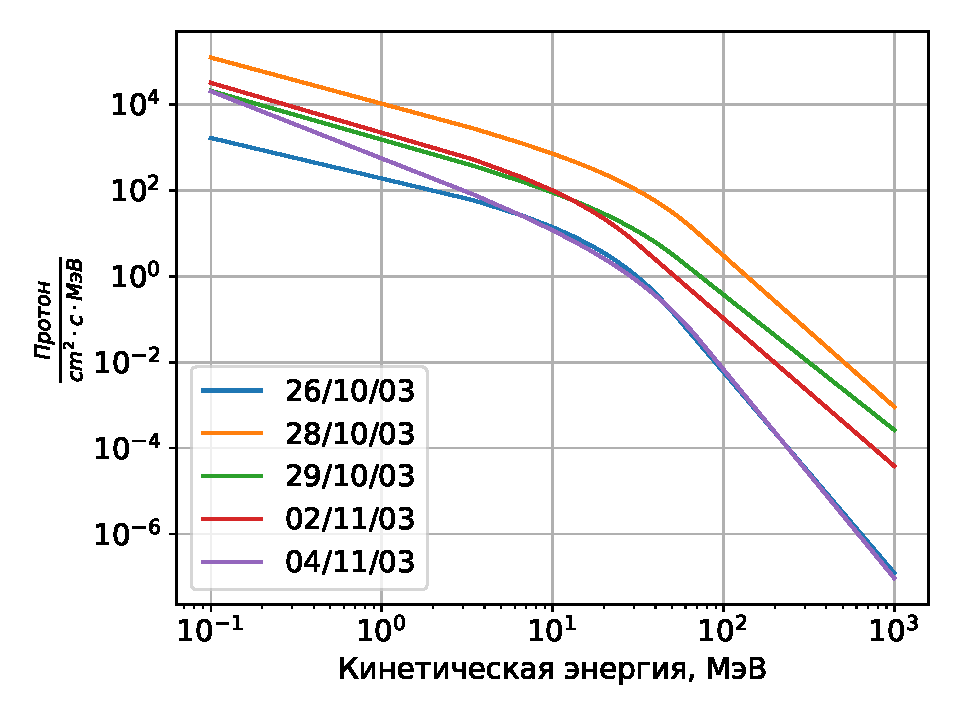
\includegraphics[width=\linewidth]{satellite/proton_spectrum.pdf} \\ а)}
        \end{minipage}
        \hfill
        \begin{minipage}[h]{0.49\linewidth}
            \center{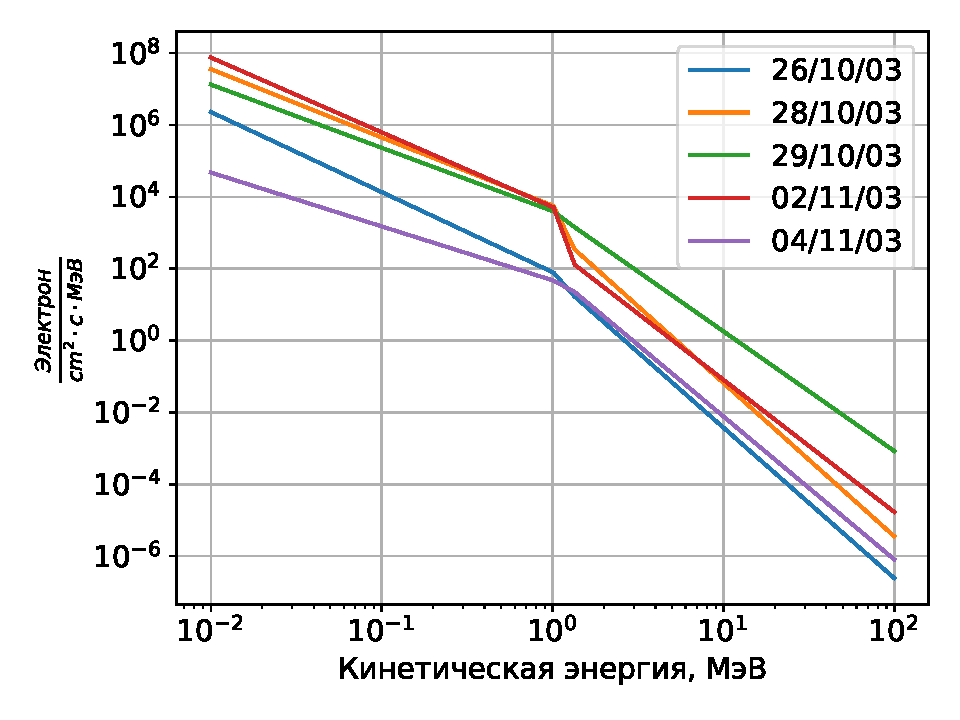
\includegraphics[width=\linewidth]{satellite/electron_spectrum.pdf}   \\ б)}
        \end{minipage}
        \caption{ Спектры в мощных солнечных событиях октября-ноября 2003 г~\cite{mewaldt2005proton}: а) протонов б) электронов.}
    \end{center}
    \label{sat:spectrum}
\end{figure}

\todo{Переход от требование к конструкции}
 
К преимуществам ППД можно отнести их компактность и высокую разрешающую способность. Однако недостатком единичного ППД является отсутствие пространственной чувствительности и возможности различения разных типов частиц. При современном уровне технологий более целесообразной является разработка телескопа на основе сегментированного сцинтилляционного детектора. Среди преимуществ сцинтилляционного детектора можно отметить следующие: 
\begin{itemize}
    \item Малое (порядка нескольких десятков  наносекунд для органических и сотен пикосекунд для неорганических сцинтилляторов) время высвечивания, позволяющее работать в одночастичном режиме в широком диапазоне скоростей счёта (ППД имеют проблемы при скоростях счета больше $10^4$ частиц в секунду ).
    \item Более высокая радиационная стойкость и долговечность по сравнению с полупроводниковыми детекторами, возможность создавать более толстые слои материала, отсутствие подложки. 
    \item Меньшее по сравнению с ППД энергетическое разрешение, тем не менее достаточное для решения поставленных перед телескопом задач. 
\end{itemize} 
Одна из проблем сцинтилляционных детекторов - необходимость для регистрации сцинтилляционного света, или габаритных и хрупких  фотоэлектронных умножителей, или лавинных фотодиодов, компактных, но имеющих худшее энергетическое разрешение, решена в настоящее время благодаря созданию кремниевых фотоумножителей (SiPM), представляющих из себя матрицы из лавинных фотодиодов. Также в отличии от ППД в которых  электроника для съема сигнала расположена в плоскости перпендикулярной оси наблюдения (и соответственно при создании сегментированного полупроводникового детектора будет подвержена радиационным повреждениям), съем сигнала с сцинтилляционных шайб возможен с торца шайбы или посредством оптоволоконного кабеля (что позволяет разделить рабочее тело детектора и электронику, укрыв её в корпусе КА).
За счет сегментации детектора и раздельного съема света с разных слоев, можно частично идентифицировать геометрию трека частицы и фильтровать события в нужном апертурном окне без использования громоздких коллиматоров. Однако небольшое апертурное устройство для выделения необходимого поля зрения помогает улучшить характеристики детектора.

\begin{figure}[ht]
    \centerfloat{
        \hfill
        \subbottom[Ионизационные потери для протонов (100 МэВ) и электронов (10 МэВ)\label{sat:bragg}]{%
            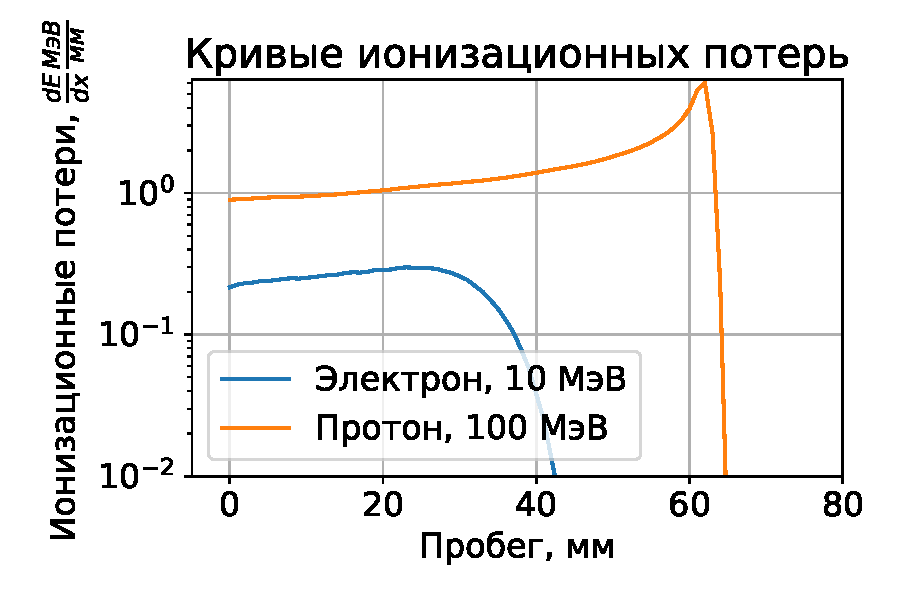
\includegraphics[width=0.4\linewidth]{satellite/01_bregg.pdf}}
        \hfill
        \subbottom[Пробег протонов и электронов\label{sat:range}]{%
            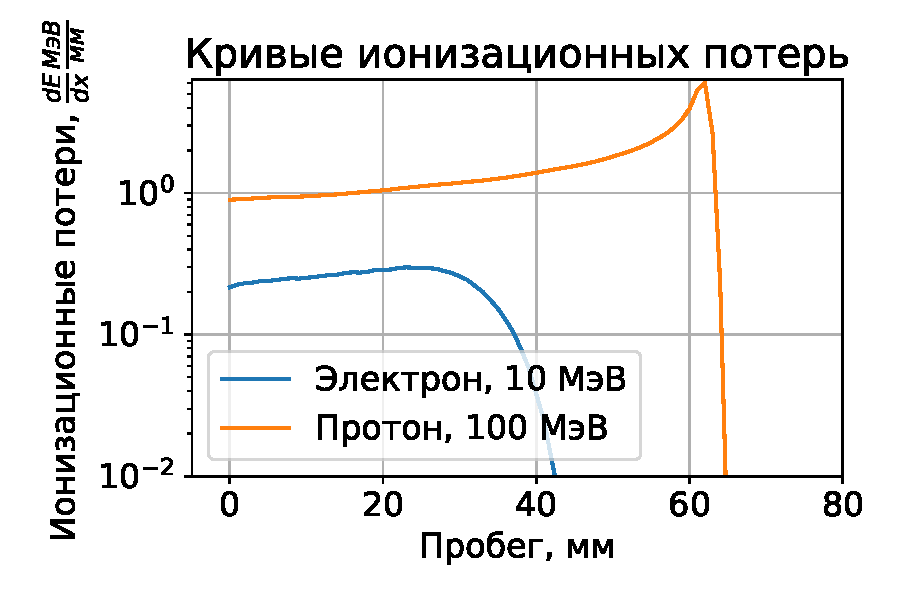
\includegraphics[width=0.4\linewidth]{satellite/01_bregg.pdf}}
        \hfill
    }
    \caption{Прохождение протонов и электронов через антрацен}\label{sat:antrachen}
\end{figure}

%\begin{figure}[t]
%    \begin{center}
%        \begin{minipage}[h]{0.49\linewidth}
%            \center{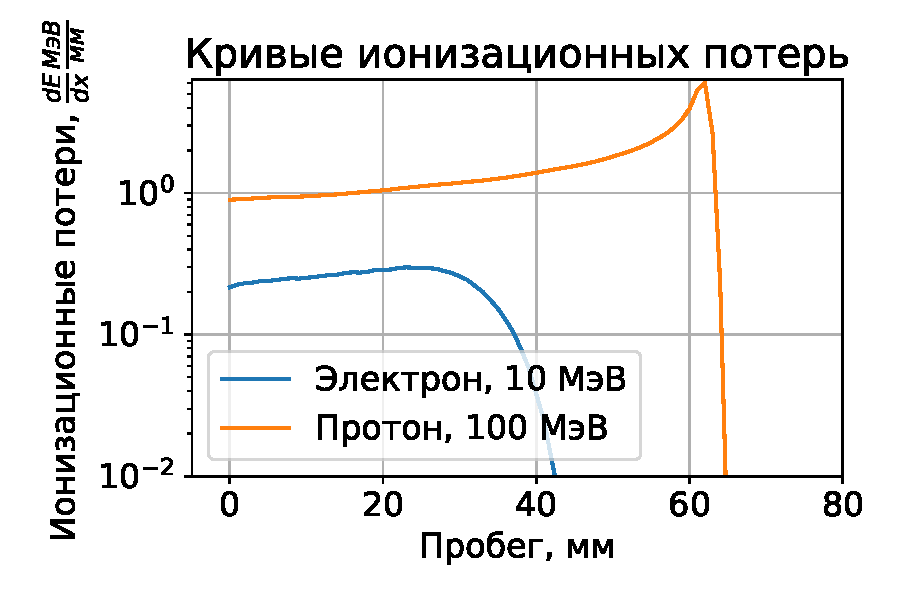
\includegraphics[width=60mm]{satellite/01_bregg.pdf} \\ а)}
%        \end{minipage}
%        \hfill
%        \begin{minipage}[h]{0.49\linewidth}
%            \center{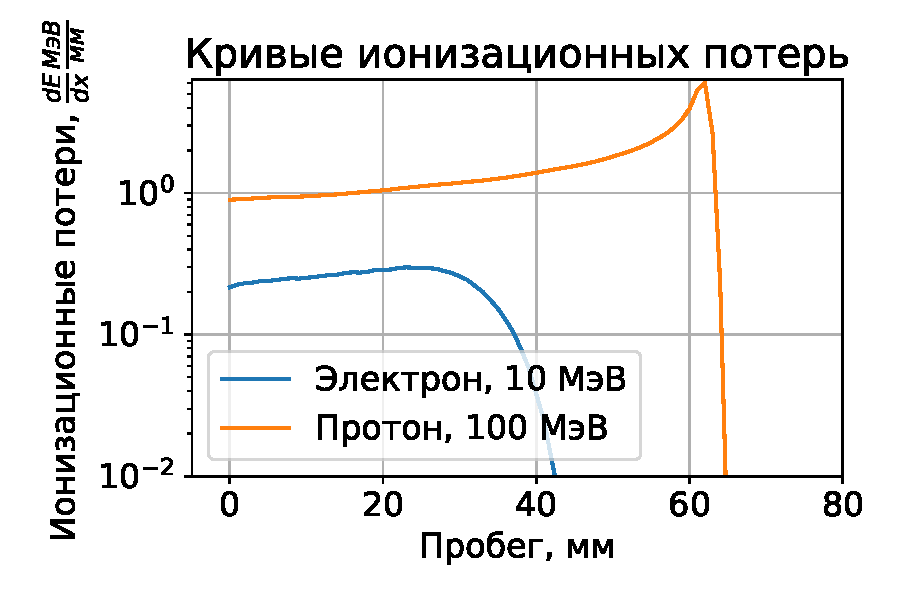
\includegraphics[width=60mm]{satellite/01_bregg.pdf}   \\ б)}
%        \end{minipage}
%        \caption{а) \todo{Спектр СКЛ} б) Ионизационные потери для протонов (100 МэВ) и электронов (10 МэВ) для антрацена.}
%    \end{center}
%    \label{sat:bregg}
%\end{figure}

Создание многослойного сцинтилляционного детектора позволяет проводить анализ не только по полной выделенной энергии, но и по форме кривой зависимости   ионизационных потерь  от пробега частицы, а также отсекать фоновые события, анализируя расположения сработавших слоев. На рисунке показаны зависимости для потерь на единицу длины в зависимости от глубины проникновения для протонов с энергией 100 МэВ и для электронов с энергией 10 МэВ. Следует отметить два факта - кривые ионизационных потерь протонов имеют характерную особенность - пик Брэгга и разницу в ионизационных потерях протонов и электронов, что позволяет, измерив зависимость энерговыделения от пробега с высокой точностью определить тип и энергию частицы. 

Телескоп представляет собой набор цилиндрических сцинтилляционных шайб, диаметром 3 см, разделенных светоотражающим материалом, помещенных в металлический корпус. В одном или нескольких местах в шайбе делается скос или “ушко” для установки фотоумножителя. Для обеспечения равномерного светосбора рассматриваются варианты с установкой до трех фотоумножителей на одну шайбу или с кольцевым оптоволокном. Места установки детекторов в последовательных шайбах могут быть сдвинуты друг относительно друга на 60° для того, чтобы слои можно было делать достаточно тонкими и детекторы в соседних слоях не мешали друг другу. Входное окно телескопа остается открытым, но при необходимости на него может быть установлен коллиматор или фильтр низкоэнергетичных частиц (например, бериллиевое покрытие). Толщина шайб может быть выбрана разной в зависимости от конкретных задач детектора (более тонкие слои позволяют получить лучшее разрешение, но при этом увеличивается вес детекторов и сопутствующей электроники). В общем случае предполагается, что вблизи входного окна плотность слоев выше, поскольку там требуется большая точность определения формы кривой потерь (для идентификации электронов).
Параметры конструкции будут меняться в зависимости от конкретной задачи и ограничений на габариты и вес прибора. Будут варьироваться следующие параметры:
Тип сцинтиллятора - более плотные сцинтилляторы позволяют создавать более компактный детектор. Также следует учесть ограничения по температурам и радиационной нагрузки, которые зависят от конструкции спутника.
Полная длина телескопа - увеличение полной длины детектора приводит к увеличению измеряемого диапазона энергий, но и увеличивает массу детектора. Надо отметить, что детектор позволяет измерять энергию частиц, которые проходят его насквозь (при помощи определения потерь на единицу длины), но точность этих измерений существенно ниже.
Радиус детектора - увеличение радиуса позволяет более точно определять энергию электронов, а также увеличивает угловую апертуру, но существенно увеличивает вес. 
Количество отдельных слоев и их толщины - увеличение количества слоев позволяет лучше определять энергию, но увеличивает весь электроники. Также слишком тонкие слои могут быть менее устойчивы к износу.

Полная длина пробега электронов и протонов в стандартном сцинтилляторе антрацене приведена на рисунке. Пробег протонов с энергией 100 МэВ около 65 мм. Причем если мы возьмем данный пробег в качестве полной длины детектора мы сможем эффективно измерять энергию протонов вплоть до 150 МэВ,  благодаря информации о форме кривой Брэгга, или же напротив мы можем сократить длину детектора, ухудшив диапазон измеряемых энергий, но при этом сократив массу. Также исходя из этого графика можно рекомендовать делать первые наиболее тонкие слои не более двух миллиметров для обеспечения эффективной регистрации электронов. Толщины наиболее толстых слоев должны быть достаточными для поглощения пика Брэгга и быть в диапазоне 5 -10 мм. Радус детектора целесообразно подбирать из диапазона 10 - 50 мм. Исходя из данных геометрических оценок масса без учета электроники может лежать в пределах 200-800 грамм.


\subsection{Методика измерения}


Идентификация и измерение параметров регистрируемых частиц основано на анализе ионизационных потерь частиц в толще сцинтиллятора.  При этом предполагаются три режима работы детектора, при низкой скорости набора событий производится анализ каждого одиночного события, а при превышении некоторого порога (обусловленного скоростью работы электроники и временем высвечивания сцинтиллятора) идет накопление суммарных потерь за некоторый промежуток времени, а затем восстанавливается энергетический спектр частиц попавших в детектор за это время. Третий режим является смешанным: в шайбах расположенных вблизи входного окна проводится измерение суммарных ионизационных потерь, а в дальних шайбах производится идентификация отдельных событий (это возможно при условии, что число частиц составляющих более высокоэнергетичных часть спектра будет меньше чем пороговая скорость счета). В качестве основы для анализа используется рассчитанные значения ионизационных потерь и набор триггеров для отсечения событий. Для расчета энерговыделения в сцинтилляционных шайбах проведено Монте-Карло моделирование при помощи транспортного кода GEATN4.  В качестве физического модели использовался модуль стандартной электромагнитной физики GeEmStandartPhysics, включающий в себя описание процессов оказывающих основное влияние на распространение частиц в детекторе: ионизационные потери и их флуктуации, упругое кулоновское рассеяние и тормозное излучение электронов.
Надо отметить, что детектор позволяет также измерять более тяжелые частицы (ионы) и отличать их от протонов (энергетический диапазон при этом сдвигается в область высоких энергий), а также с пониженной эффективностью частицы сверхвысоких энергий и гамма-кванты.
\subsection{Одночастичный режим}
В одночастичном режиме анализ проводится следующим образом. Для анализа отбираются события прошедшие через входное окно (иначе говоря инициирующие срабатывания сцинтилляторов начиная с первого слоя). После чего исходя из полной измеренной энергии и количества сработавших слоев определяется диапазоны возможных параметров частицы, а также отсекаются события пришедшие под большими углами. В данных диапазонах параметров определяется набор параметров максимизирующей значение функции правдоподобия --- произведения вероятностей наблюдать измеренное энерговыделение при данном наборе параметров. Процедура восстановления энергии в настоящее время дорабатывается, но предварительный алгоритм позволяет определить энергию протонов с точностью 1 МэВ для исходной энергии 50 МэВ, то есть дает точность порядка 2\%. Предполагается, что в дальнейшем точность восстановления будет улучшена в 1.5 - 2 раза за счет фильтрации событий под большими углами. Реальная чувствительность будет несколько меньше за счет неидеальности светосбора и уменьшения количества шайб, но при любых конфигурациях детектора, разрешающая способность детектора будет не хуже 10\%.
\subsection{Интегральный режим}
Для анализа спектра в интегральном режиме будет использоваться методика регуляризации обратных задач, разработанная В. Ф. Турчиным, которая позволяет без потери точности строить решение обратной интегральной задчи. Другими словами, она позволяет из интегрального спектра, содержащего протоны и электроны разной энергии выделять дифференциальные спектры для различных типов частиц. В качестве референсных кривых поглощения для восстановления используются данные моделирования. В дальнейшем планируется для этого использовать данные калибровочных измерений на протонном ускорителе Московской Мезонной Фабрики в Троицке.
В настоящее время проводится доработка математического аппарата и программной базы для анализа в интегральном режиме. Предварительные результаты восстановления спектра дают точность до 5\% в зависимости от диапазона измерений. Важно отметить, что интегральная методика применима при очень высоких загрузках детектора (свыше 1 МГц).
\subsection{Обсуждение результатов}
Разработана концепция секционного сцинтилляционного телескопа для регистрации электронов и протонов солнечного происхождения. Произведены работы по моделированию детектора и сделаны оценки его чувствительности для различных частиц и в различных диапазонах энергий. Предварительные результаты показывают, что при весе до 1 кг, детектор сможет позволить измерение энергетического спектра протонов от 5 до 100 МэВ и электронов от 1 до 10 МэВ с точностью порядка 1-5\%.
Существенным преимуществом детектора является возможность работы в так называемом интегральном режиме, когда не регистрируются индивидуальные частицы, а идет анализ полного пространственного спектра потерь энергии. Интегральный режим позволяет работать при сверхвысоких скоростях счета, обеспечивая при этом достаточно хорошую (около 5\%) точность восстановления исходного спектра и состава излучения.



\section{Проектирование сканеров основанных на использовании рентгеновского и гамма излучения
}\label{sec:detectors/scanners}

\todo{Пересказать этот раздел другими словами что бы не считалось плагиатом из статьи}

\subsection{Введение}

Для обеспечения национальной безопасности важен контроль перемещения опасных или стратегически важных грузов, таких как взрывчатые вещества, радиоактивные материалы, редкие и драгоценные металлы. Проводить такой контроль можно, сканируя содержимое транспортных контейнеров гамма-излучением.

В данной работе рассмотрена существующая методика дуальных энергий и предложен альтернативный способ, основанный на измерении энергетического распределения гамма-квантов. Для оценки было проведено моделирование с помощью транспортного кода GEANT4.  Также выполнен эксперимент по измерению энергетического разрешения детектора на основе сцинтиллирующего кристалла BGO и кремневого фотоумножителя.

Использование высокоэнергетического гамма-излучения в прикладной томографии на данный момент широко распространено.  В этой статье мы рассмотрим возможности улучшения существующего метода как путем модернизации оборудования, так и путем разработки математических алгоритмов, которые более полно используют информацию, содержащуюся в измеренных значениях. В начале мы рассмотрим существующий метод дуальных энергий и определим возможные направления для создания более точной методики. Далее в работе приведено описание нескольких симуляций и численных экспериментов с обсуждением результатов. Также в работе приведены результаты измерений характеристик сцинтилляционного кристалла BGO, который может послужить основой для модернизированного оборудования.
 
\subsection{Метод дуальных энергий}
\begin{figure}[t]
    \begin{center}
        \begin{minipage}[h]{0.49\linewidth}
            \center{ \includegraphics[width=0.99\linewidth]{scanner/Attenuation.pdf}  \\ а)}
        \end{minipage}
        \hfill
        \begin{minipage}[h]{0.49\linewidth}
            \center{ \includegraphics[width=0.99\linewidth]{scanner/Bremsstrahlung.pdf}  \\ б)}
        \end{minipage}
        \caption{а) Массовый коэффициент ослабления для различных материалов. б) Спектр тормозного излучения от электрона с энергией 10 МэВ.}
    \end{center}
    \label{pic:att}
\end{figure}

Рассмотрим, как уменьшается поток гамма-лучей. Коэффициент пропускания описывается следующим уравнением:
\begin{equation}
\label{eq:trans}
T(E_0, t, Z) = \frac{\int \limits_0^{E_0} S(E_0, E) \exp(-\mu(E,Z)\times t)~dE)}{\int \limits_0^{E_0} S(E_0, E)~dE},
\end{equation}
где $T$ --- прозрачность материала для гамма-излучения, $S(E_0, E)$ --- функция отклика детектора, $\mu(E,Z)$ --- массовый коэффициент ослабления, $t$ ---  оптическая толщина материала, $E_0$ --- предельная энергия тормозного излучения, $E$ --- энергия гамма-излучения, $Z$ --- заряд ядра исследуемого материала.

Предположим, что в качестве источника гамма-лучей используется тормозное излучение со спектром как на рисунке~\ref{pic:att}б и максимальной энергией $E_0$, зависящей от энергии электронного пучка. Коэффициент прозрачности  $T(E_0, t, Z)$ также зависит от среднего массового коэффициента ослабления материала. Рисунок~\ref{pic:att}а показывает зависимость коэффициента ослабления от энергии для различных материалов. Мы можем выделить три области: начальную, в которой доминирует фотоэлектрический эффект и могут быть разделены только материалы с большим зарядом ядра; среднюю, в которой доминирует комптоновское рассеяние и материалы не различимы,и наконец область, где основное влияние оказывает процесс рождения электрон-позитронных пар и материалы достаточно хорошо различимы~\cite{geheitler1984quantum, spirin, Geant2016}. Последняя область может быть использована для метода дуальных энергий~\cite{spirin}.

Уравнение~\ref{eq:trans} не позволяет определить материал, если неизвестна оптическая толщина материала. Для решения этой проблемы в методе дуальной энергии предлагается использовать два электронных пучка с различной энергией. Используя прозрачность для двух предельных энергий гамма-лучей $E^{(1)}_0$ и $E^{(2)}_0$, а затем минимизируя функционал
\begin{equation}
F(z) = \frac{|t(E^{(1)}_0,z) - t(E^{(2)}_0,z)|}{t(E^{(1)}_0,z)} \to min,
\end{equation}
становиться возможным исключить неизвестную нам оптическую толщину и вычислить эффективное зарядовое число для исследуемого материала. Данный метод позволяет отнести сканируемый материал к одной из четырёх групп, разделённых по эффективному зарядовому числу: $Z_{eff} \sim 5$, $Z_{eff} \sim 13$, $Z_{eff} \sim 26$, $Z_{eff} \sim 82$.\\
Однако, метод дуальной энергии имеет некоторые недостатки, среди которых мы выделим два:
\begin{itemize}
    \item Необходимость в двух пучках различной энергии ведет к усложнению конструкции сканера.
    \item Данный метод будет иметь малую эффективность в случае материала, состоящего из сильно различающихся по заряду элементов.
\end{itemize}
Поэтому мы предлагаем альтернативный подход:
\begin{itemize}
    \item Использовать только один электронный пучок с энергией 10~МэВ.
    \item Измерять не только пространственное, но и энергетическое распределение гамма-квантов.
\end{itemize}

\subsection{Моделирование}
\begin{figure}[t]
    \begin{center}
        \includegraphics[width=120mm]{scanner/yed_schema_1.pdf}
        \caption{Схема симуляции}
    \end{center}
    \label{pic:schema1}
\end{figure}
Для оценки мы провели несколько GEANT4~\cite{Geant2016, Geant2006, Geant2003} симуляций, используя схему (рис.~\ref{pic:schema1}): электронный пучок с энергией 10~МэВ сталкивается с вольфрамовым конвертором, создавая тормозное излучение, которое облучает стальной двухметровый контейнер, внутри которого находится сканируемый объект и регистрируется детектором. Расстояние между вольфрамовым конвертором и контейнером составляет два метра, между контейнером и детектором --- 10~см.

Приведем несколько примеров проведенного моделирования:
\begin{itemize}
    \item На рисунке~\ref{pic:sword}а показан пример опасного стального объекта неоднородной толщины, сравнимой с толщиной стенок контейнера.
    \item Рисунки~\ref{pic:sword}б и~\ref{pic:hex}а показывают результат моделирования уранового кубика с ребром 6~сантиметров (вес около 4~кг), помещенного в свинцовую сферу толщиной 1~см. Как показало моделирование, такой куб можно обнаружить с толщиной оболочки до 5~сантиметров.
    \item Рисунок~\ref{pic:hex}б демонстрирует разницу между двумя органическими материалами: безопасным --- целлюлозой и опасным --- гексогеном (RDX). Разница значительна, это означает, что можно разработать алгоритмы поиска органических взрывчатых веществ.
    \item На рисунке~\ref{pic:diff}б показан результат сравнения двух энергетических спектров (в качестве сравнительной метрики выбран логарифм отношения интенсивностей) для сфер из алюминия и урана диаметром 1~см. Как видим, даже в таких малых масштабах и малых (по сравнению с реальным пучком) интенсивностях можно регистрировать различия в энергетических спектрах.
\end{itemize}
\begin{figure}[t]
    \begin{center}
        \begin{minipage}[h]{0.49\linewidth}
            \center{\includegraphics[width=0.99\linewidth]{scanner/Sword.pdf} \\ а)}
        \end{minipage}
        \hfill
        \begin{minipage}[h]{0.49\linewidth}
            \center{ \includegraphics[width=0.99\linewidth]{scanner/UranCube1.pdf} \\ б)}
        \end{minipage}         
        \caption{а) Опасный стальной предмет с неравномерной толщиной. б) Кубик урана в свинцовой оболочке (XY-распределение).}
    \end{center}
    \label{pic:sword}
\end{figure}
\begin{figure}[t]
    \begin{center}
        \begin{minipage}[h]{0.49\linewidth}
            \center{\includegraphics[width=0.99\linewidth]{scanner/UranCube2.pdf}  \\ а)}
        \end{minipage}
        \hfill
        \begin{minipage}[h]{0.49\linewidth}
            \center{\includegraphics[width=0.99\linewidth]{scanner/Hex.pdf} \\ б)}
        \end{minipage}
        \caption{а) Кубик урана в свинцовой оболочке (X-распределение). б) Сравнение целлюлозы и гексогена.}
    \end{center}
    \label{pic:hex}
\end{figure}
\begin{figure}[t]
    \begin{center}
        \begin{minipage}[h]{0.49\linewidth}
            \center{\includegraphics[width=0.99\linewidth]{scanner/diffmat0.pdf} \\ а)}
        \end{minipage}
        \hfill
        \begin{minipage}[h]{0.49\linewidth}
            \center{\includegraphics[width=0.99\linewidth]{scanner/diffmat.pdf}  \\ б)}
        \end{minipage} 
        \caption{а) Энергетические спектры различных материалов (общий вид).
            б) Энергетические спектры различных материалов (участок с энергией более 4~МэВ).}
    \end{center}
    \label{pic:diff0}
\end{figure}
\begin{figure}[t]
    \begin{center}
        \begin{minipage}[h]{0.49\linewidth}
            \center{\includegraphics[width=0.99\linewidth]{scanner/diffmat1.pdf}  \\ а)}
        \end{minipage}
        \hfill
        \begin{minipage}[h]{0.49\linewidth}
            \center{\includegraphics[width=0.99\linewidth]{scanner/Difference.pdf}   \\ б)}
        \end{minipage}
        \caption{а) Зависимость метрики от эффективного зарядового числа материала.
            б) Сравнение энергетических спектров из урановых и алюминиевых сфер.}
    \end{center}
    \label{pic:diff}
\end{figure}

Чтобы оценить возможность определения эффективного заряд материала по энергетическому спектру, было смоделировано сканирование шести мишеней из различных материалов (железо, свинец, алюминий, целлюлоза, олово, уран) с одинаковыми поперечными и различными продольными размерами. Продольный размер был выбран таким образом, чтобы общее ослабление потока гамма-излучения было одинаковым для всех материалов, и их нельзя было различить только путем анализа количества гамма-квантов пришедших в детекторы.

Энергетические спектры этих мишеней показаны на рисунках. Как видно, спектры для всех мишеней различны в области до 3~МэВ (см. рис.~\ref{pic:diff0}a) и в области после 4~МэВ (см. рис.~\ref{pic:diff0}б). Следует отметить, что это различие является значительным даже при малых интенсивностях электронного пучка ($10^8$ электронов), что указывает на более выраженное различие в реальном электронном пучке от ускорителя ($10^{15}$ электронов). Таким образом, можно сформулировать простой критерий, отличающий различные материалы: доля числа частиц с энергией больше 3~МэВ. Такой критерий позволяет отличать материалы по $Z_{eff}$ (см. рис~\ref{pic:diff}а). Следует отметить, что ошибки на рисунке~\ref{pic:diff} являются только статистическими и при интенсивностях, соответствующих реальному электронному пучку, будут незначительны.

Сформулированный критерий достаточно хорош для практического использования, однако он не является оптимальным решением, поскольку при его использовании большая часть информации о спектре теряется. В следующем разделе мы использовали простой пример, чтобы показать потенциал для создания трехмерной гамма-томографии с использованием полной информации о спектре.

\subsection{Восстановление толщин материалов}
Рассмотрим одномерный случай, когда гамма-лучи проходят стопку из нескольких материалов с фиксированной общей толщиной, и нам нужно восстановить толщину отдельных материалов (см. схему~\ref{schema2}). Мы используем простую модель, в которой ослабление потока гамма-излучения задается следующим уравнением
\begin{equation}
\label{eq:gamma}
\frac{N(E)}{N_0(E)} = \exp(-\sum_i \Sigma^{mean}_i(E)x_i),
\end{equation}
где $x_i$ --- толщина $i$-слоя, $\Sigma^{mean}_i$ --- среднее макроскопическое сечение для группы материалов с близкими зарядовыми числами, $N,~N_0$ --- количество гамма-квантов. В этом случае мы не учитываем многократное рассеяние и наличие аннигиляционной линии. Мы считаем, что общая толщина известна и для восстановления толщины отдельных слоев мы используем метод наименьших квадратов, т. е. минимизируем такую сумму:
\begin{equation}
\sum_E(\ln \frac{N(E)}{N_0(E)} + \sum_i \Sigma^{mean}_i(E)x_i))^2 \to min
\end{equation}

Приведем пример работы алгоритма. Мы будем считать, что энергетическое разрешение составляет величину 10\%. Рассмотрим стопку из трех слоев: алюминиевого, железного и свинцового. Рисунок~\ref{rec:ex}а показывает вклад каждого восстановленного материала в общее ослабление потока гамма-лучей. Таблица~\ref{tab:rec} содержит результаты восстановления для данного примера. Как мы видим из таблицы, результат восстановления довольно точный.Чтобы прояснить возможности алгоритма, мы провели несколько численных экспериментов. Мы также как и в примере использовали алюминий, железо и свинец, и взяли около двухсот наборов с разным соотношение толщин слоев, причем суммарная толщина лежала в диапазоне от 30 до 180~сантиметров.
\begin{figure}[ht] 
    \centerfloat{
    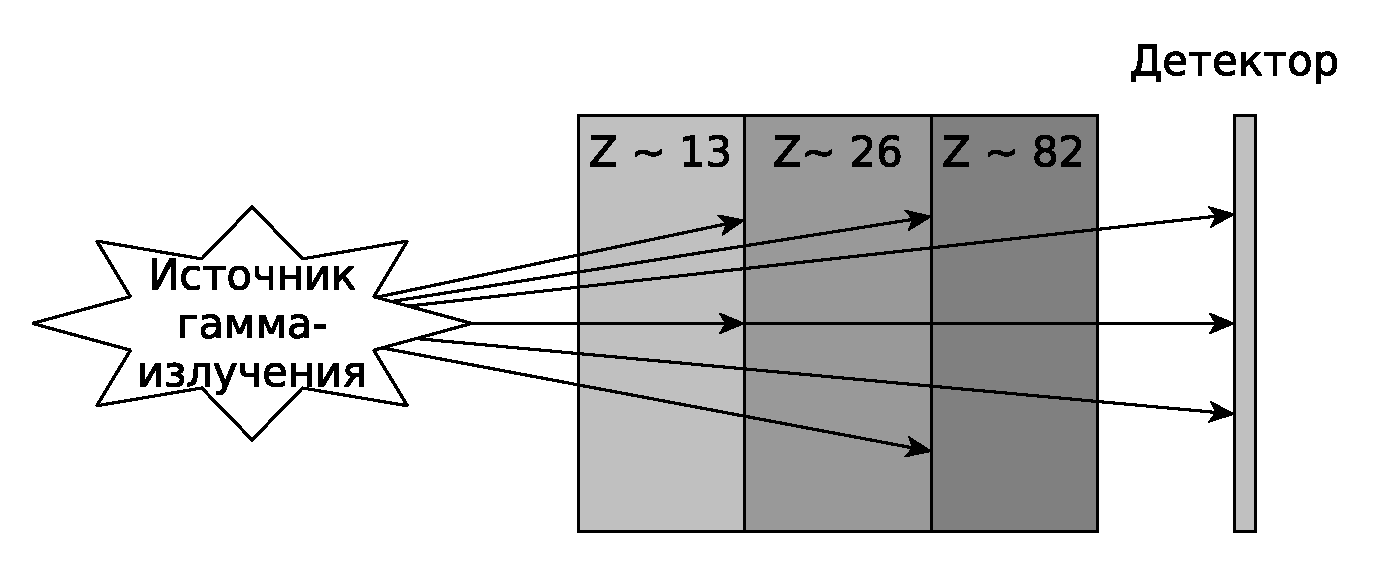
\includegraphics[width=\linewidth]{scanner/yed_schema_2.pdf}
    \caption{Восстановление толщин материалов (схема моделирования).}
    \label{schema2}
}
\end{figure}
Рисунок~\ref{rec:ex}б показывает разброс ошибки восстановления для данных наборов. Как мы можем видеть толщина тяжелых элементов определяется лучше всего: с точность порядка 5\%, а толщина элементов из группы железа хуже всего: величина ошибки достигает 30\%. Однако, мы рассматривали весьма простую модель и возникает вопрос: какая от неё польза? В данной модели мы использовали только энергетическое разрешение и по нему смогли провести восстановление послойной структуры объекта. При добавлении пространственного распределение, мы можем провести дополнительно сегментирование вдоль ещё одной оси и с учетом временной компоненты восстановить трехмерную структуру груза контейнера (3D гамма-томография). Таким образом наша простая модель показывает, что у нас есть перспектива создания действительно мощной системы для анализа содержимого контейнеров.

\begin{figure}[t]
    \begin{center}
        \begin{minipage}[h]{0.49\linewidth}
            \center{\includegraphics[width=0.99\linewidth]{scanner/reconstruction.pdf} \\ а)}
        \end{minipage}
        \hfill
        \begin{minipage}[h]{0.49\linewidth}
            \center{\includegraphics[width=0.99\linewidth]{scanner/relError.pdf}   \\ б)}
        \end{minipage}
        \caption{а) Вклад отдельных слоев в полное ослабление потока. б) Распределение ошибок восстановления для различных численных экспериментов.}
    \end{center}
    \label{rec:ex}
\end{figure}

\begin{table}
    \caption{Пример результата  работы алгоритма восстановления}
    \label{tab:rec}
    \begin{center}
        \begin{tabular}[c]{|c|c|c|}
            \hline 
            Материал & Истинная толщина, см & Восстановленная, см \\ 
            \hline 
            Al & 20 & 19.6 \\ 
            \hline 
            Fe & 40 & 41.6 \\ 
            \hline 
            Pb & 30 & 28.7 \\ 
            \hline 
        \end{tabular}
    \end{center}
\end{table}

\newpage
\subsection{Измерение энергетического разрешения детектора}
В дополнение к моделированию, было измерено энергетическое разрешение сцинтилляционного детектора гамма-излучения. В качестве сцинтиллятора использовался кристалл BGO размером 10x30x100~мм (глубина кристалла подбиралась так, чтобы обеспечить полное поглощение гамма-квантов до 10~МэВ), для регистрации излучения сцинтиллятора использовался фотодетектор ArrayC-60035-4P. В качестве источников излучения использовались $^{22}Na$ (имеет две линии 0.511~МэВ и 1.275~МэВ) и $^{137}Cs$ (имеет линию 0.662~МэВ). Фотодетектор ArrayC-60035-4P  представляет из себя матрицу из четырёх фотодиодов размером 6x6~мм, оснащенную индивидуальным предусилителем с коэффициентом усиления равным 150. В процессе работы измерялся суммарный сигнал с двух фотодиодов матрицы. Сигнал c матрицы подавался на усилитель (ORTEC~579) и затем поступал на входной канал АЦП (CAEN~DT5742) и на дискриминатор (CAEN mod. 224), логический сигнал которого служил триггером в системе. В отсутствие источника шкала АЦП была прокалибрована в абсолютных единицах --- числе фотоэлектронов. В таблице~\ref{tab:ex} представлен результат измерения разрешения детектора ---  отношения СКО фотопика к его положению ($\frac{\sigma_E}{E}$). Световыход составляет 140 фотоэлектронов на МэВ, а порог шумов --- величину порядка 100~кэВ.\\
\begin{table}
    \caption{Измерение энергетического разрешения детектора}
    \label{tab:ex}
    \begin{center} 
        \begin{tabular}[c]{|c|c|c|}
            \hline 
            Источник & Энергия, МэВ & $\frac{\sigma_E}{E}$\\
            \hline 
            $^{22}Na$&0.511 & 19.0 \%  \\ 
            \hline 
            $^{137}Cs$&0.662 & 14.7\%\\ 
            \hline 
            $^{22}Na$& 1.275 & 13\% \\
            \hline 
        \end{tabular} 
    \end{center}
\end{table}


\subsection{Обобщение результатов и обсуждение дальнейших перспектив разработки}
Результаты:   
\begin{enumerate}
    \item Энергетические спектры материалов с различным эффективным зарядовым числом различаются в областях энергий до 3 и после 4~МэВ. Оценена зависимость зарядового числа от доли гамма-квантов с энергией выше 3~МэВ. Данный метод позволяет идентифицировать в контейнере отдельные группы элементов по зарядовому числу (легкие, средние, тяжелые) в одной экспозиции при одной фиксированной энергии электронов, оптимально вблизи 8~МэВ. При этом требуется разрешение не хуже 15\% и эффективность регистрации около 90\%. 
    \item Энергетическое разрешение порядка 10\% позволяет определить толщину отдельного слоя в многослойной структуре с точностью 25\%.
    \item Измерено энергетическое разрешение детектора на основе BGO, в целом полученные результаты говорят о высоких эксплуатационных характеристиках и качестве материала. Представляется возможным достижение характеристик заявленных производителем ($FWHM \sim 9\%$ для $^{137}Cs$).
\end{enumerate}

Развитие данной тематике является перспективным направлением деятельности, но требует финансовой поддержки, при наличии которой становиться возможным разработка программы для проверки содержимого транспортного контейнера по заявленному манифесту, и создание программы для гамма-томографии содержимого контейнеров.

%Данная работа частично профинансирована в рамках госзадания № 3.3008.2017/ПЧ Министерства Образования и Науки Российской Федерации, и частично выполнена при поддержке гранта РНФ № 16-12-10039.
           % Глава 2
\chapter{Моделирование TGE и TGF
}\label{ch:thunderstorm}

\section{Обзор экспериментальных результатов
}\label{sec:thunderstorm/review-exp}

\section{Обзор существующих моделей}\label{sec:thunderstorm/review-mod}

\section{Моделирование RREA, сравнение с результатами Гуревича, Орешкина.}\label{sec:thunderstorm/rrea}
\section{Расчет коэффициента обратной связи, сравнение с результатами Дваера}\label{sec:thunderstorm/rdfm}
\section{Reactor like TGE-model}\label{sec:thunderstorm/reactor}
\clearpage            % Глава 3
\section{Расчет коэффициента обратной связи, сравнение с результатами Дваера}\label{sec:thunderstorm/rdfm}

Несмотря на то что в хороших условиях в лавине убегающих электронов может быть сгенерировано более миллиона дополнительных электронов, это не объясняет большие потоки гамма-квантов в TGF, а также не дает объяснения как связанны между собой процессы с высокоэнергетичными частицами и разряды молнии. Одним из вариантов модификации теории Гуревича, является построение на её основе модели с обратной связью (ОС). Джозеф Дуайер в работе~\cite{dwyer2003fundamental} предложил рассмотреть два механизма которые могут привести к возникновению обратной связи: гамма обратная связь возникает за счет того что не смотря на то что рождаемые убегающими электронами гамма-квант имеют начальный импульс сонаправленный с направление движения лавины, часть из них в результате рассеяния может в итоге оказаться в части облака в котором начиналась лавина и выбить там электрон, который станет новым затравочным электроном, позитронная обратная связь возникает за счет конверсии гамма-квантов электрон-позитронные пары, при этом позитрон имеет шанс развернутся в электрическом поле и начать ускорятся против направления распространения лавины, выбивая вторичные электроны, которые опять же имеют шанс развернутся в электрическом поле и стать новым затравочным электроном. Рисунок проведенного мною моделирования, иллюстрирует описание позитронной обратной связи: красные треки отображают лавину убегающих электронов, зеленные треки тормозные гамма-кванты, синий трек показывает позитрон обратной связи, который как мы видим создает новые затравочные электроны (которые правда не создают новую лавину). Механизмы описанные Дуайером должны работать в широком диапазоне атмосферных условий, однако являются вероятностными и возникает вопрос насколько значителен вклад этих механизмов в развитие лавин убегающих электронов. В работе~\cite{skeltved2014} повторялись результаты Дуайера, однако без углубленного анализа. В данной работе мы попробуем глубже рассмотреть работу этих механизмов.

\begin{figure}[ph!]
    \begin{center}
        \includegraphics[width=\linewidth]{thunderstorm/ayss_2018_art/10_dwyer.pdf}
        \caption{Распространение лавины убегающих электронов, красные треки --- электроны, зеленые треки --- гамма-кванты, синий трек --- позитрон.}
    \end{center}
    \label{fig:storm:dwyer}
\end{figure}

В работе~\cite{dwyer2003fundamental} приводятся результаты моделирования при нормальных условиях исследующие при каких соотношениях длины области с электрическим полем и величины поля может возникать обратная связь. Синяя линия на графике~\ref{fig:storm:dwyer2003} отображает результат полученный Дуайером в ~\cite{dwyer2003fundamental} при значения электрического поля и длины выше этой кривой возникает положительная обратная связь, которая ведёт к значительному росту новых затравочных частиц, который приводит в возникновению TGF и активной ионизации облака достаточной для разряда молнии, в частности подобный результат также говорит что внутри облаков не должно быть скрытых областей с сильным полем --- подобные области должны быстро разряжаться в следствии действия механизмов обратной связи.

Для проверки данных результатов было проведено собственное моделирование, состоящее из двух частей:
\begin{itemize}
	\item Моделирование рождения новых затравочных электронов (аналогично работе~\cite{dwyer2003fundamental} электрон считался новым затравочным, если рождался в от гамма-кванта или позитрона в верхней половине облака)за счет гамма и позитронной обратной связи за одну итерацию на одну первичную частицу.
	\item Расчет вероятности с которой электрон может развернутся в электрическом поле. 
\end{itemize}
Для оценки вероятности разворота было проведено GEANT4 моделирование, для сухого воздуха при нормальных условиях, величины электрического поля бралась от 5 до 10 кВ/см с шагом 0.5 кВ/см. Результат расчета вероятности разворота представлена на рисунках~\ref{fig:storm:reverse_nc_1} и ~\ref{fig:storm:reverse_nc_2}. Так же что бы быть уверенным что электрон после разворота сможет начать движение была рассчитана средняя энергия электрона после разворота, результаты приведены на графиках~\ref{fig:storm:reverse_energy_nc_1} и ~\ref{fig:storm:reverse_energy_nc_2}, как видно из графиков хоть электрон и тратит энергию на разворот, она остается достаточной для запуска новой лавины убегающих электронов (см. график TODO(график), показывающий минимальную энергию для начала убегания).  

\begin{figure}[ph!]
    \begin{center}
        \begin{minipage}[h]{0.49\linewidth}
            \center{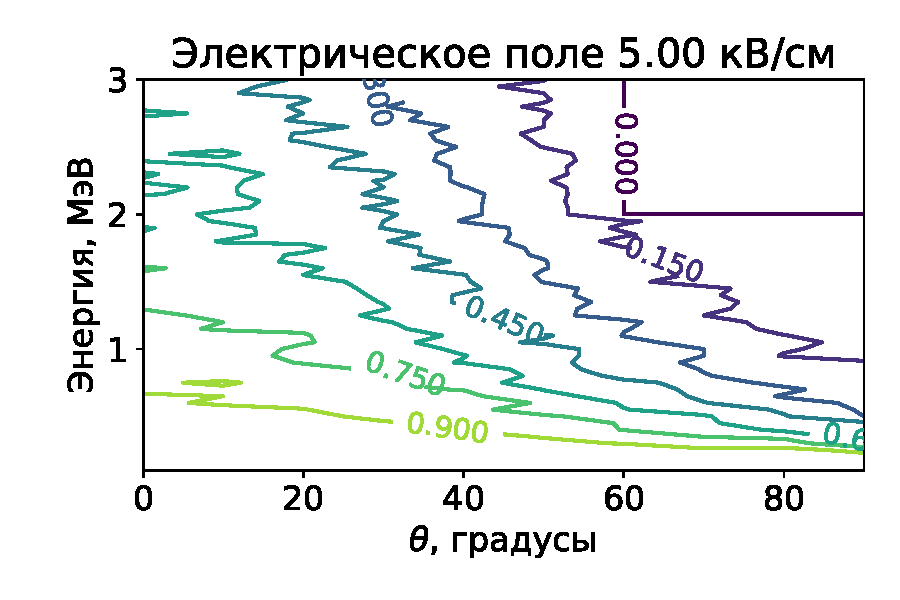
\includegraphics[width=\linewidth]{thunderstorm/rdfm/reverse_5_00.pdf} \\ а)}
        \end{minipage}
        \hfill
        \begin{minipage}[h]{0.49\linewidth}
            \center{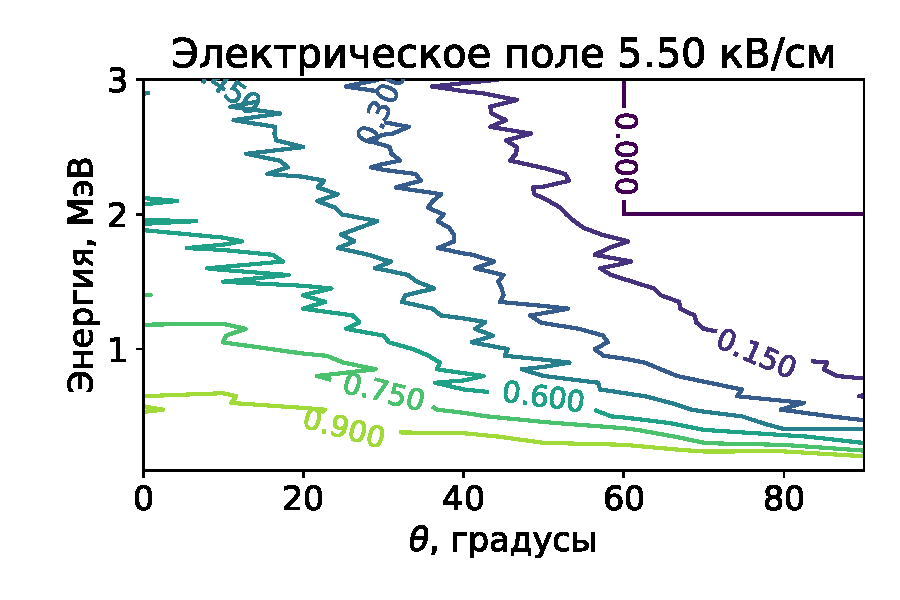
\includegraphics[width=\linewidth]{thunderstorm/rdfm/reverse_5_50.pdf} \\ б)}
        \end{minipage}
        \vfill
        \begin{minipage}[h]{0.49\linewidth}
            \center{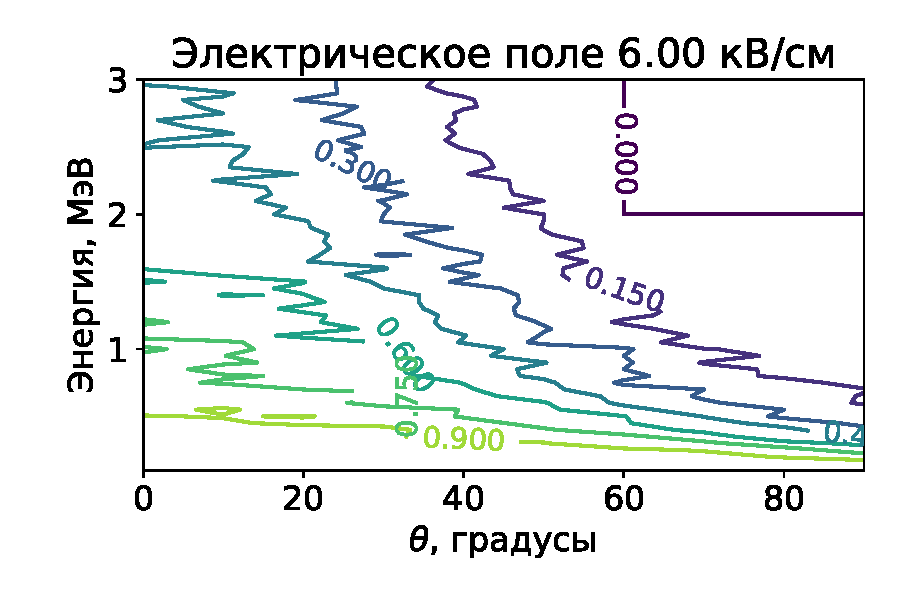
\includegraphics[width=\linewidth]{thunderstorm/rdfm/reverse_6_00.pdf} \\ в)}
        \end{minipage}
        \hfill
        \begin{minipage}[h]{0.49\linewidth}
            \center{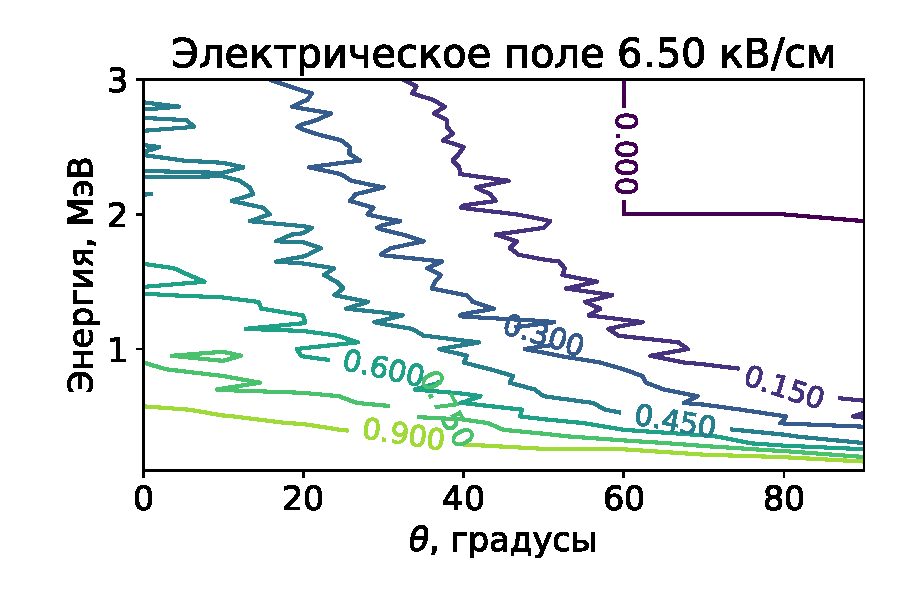
\includegraphics[width=\linewidth]{thunderstorm/rdfm/reverse_6_50.pdf} \\ г)}
        \end{minipage}
        \vfill
        \begin{minipage}[h]{0.49\linewidth}
            \center{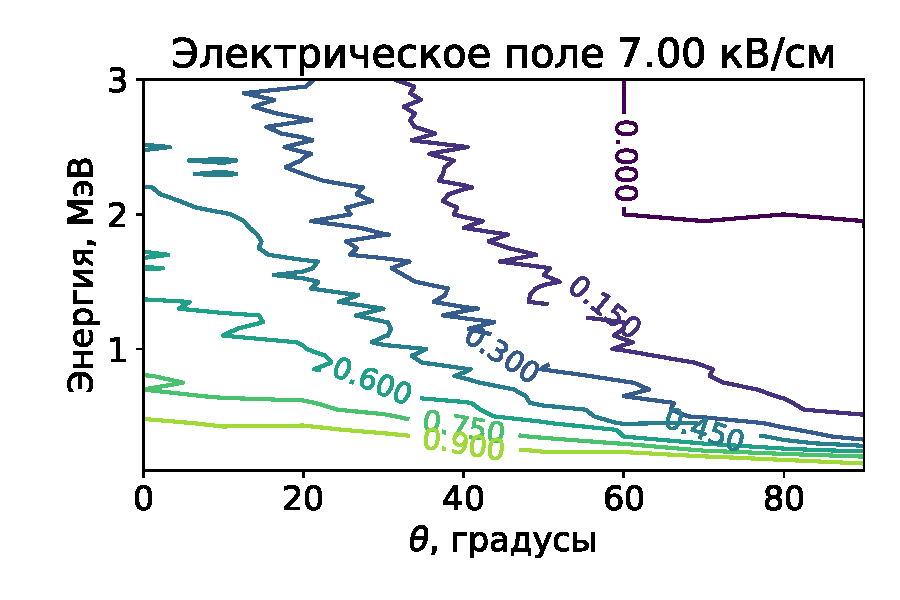
\includegraphics[width=\linewidth]{thunderstorm/rdfm/reverse_7_00.pdf} \\ д)}
        \end{minipage}
        \hfill
        \begin{minipage}[h]{0.49\linewidth}
            \center{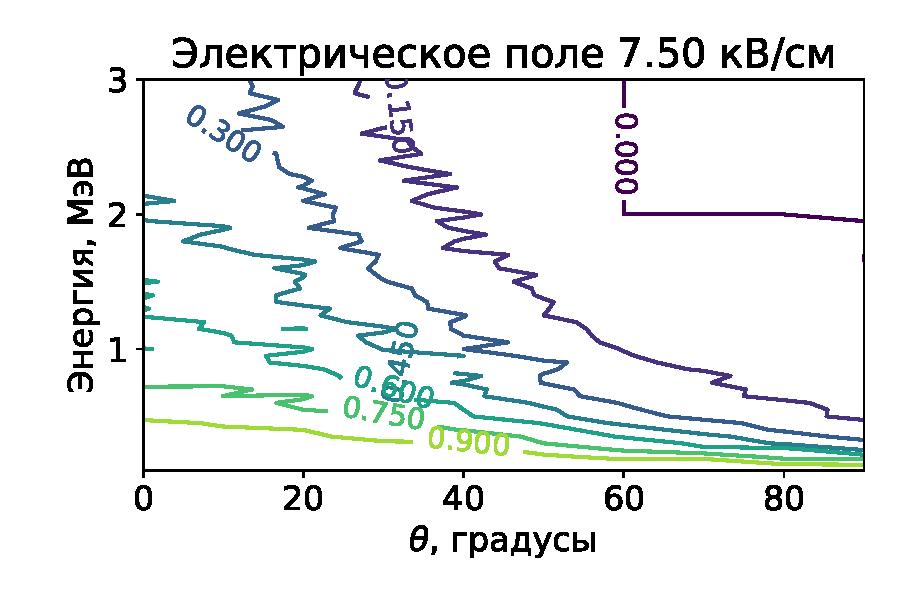
\includegraphics[width=\linewidth]{thunderstorm/rdfm/reverse_7_50.pdf} \\ е)}
        \end{minipage}
        \caption{Расчет вероятности электрона развернутся в электрическом поле для нормальных условий. По оси X отображается угол между направление движения TODO(перерисовать угол на графике), а по оси Y энергия электронов. На графики отображены линии с постоянной вероятность разворота и числовое значение вероятности на линии.}
    \end{center}
    \label{fig:storm:reverse_nc_1}
\end{figure}
\begin{figure}[ph!]
    \begin{center}
        \begin{minipage}[h]{0.49\linewidth}
            \center{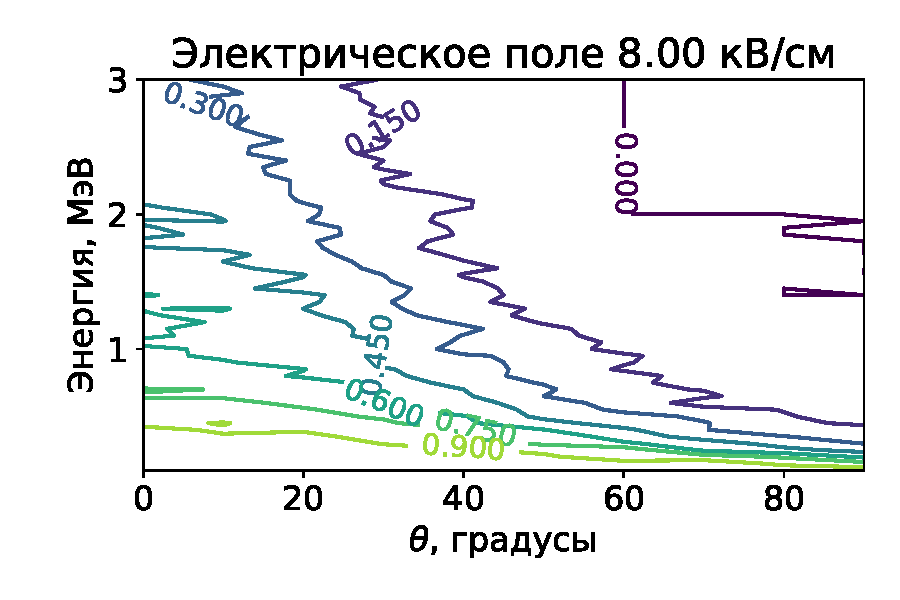
\includegraphics[width=\linewidth]{thunderstorm/rdfm/reverse_8_00.pdf} \\ ж)}
        \end{minipage}
        \hfill
        \begin{minipage}[h]{0.49\linewidth}
            \center{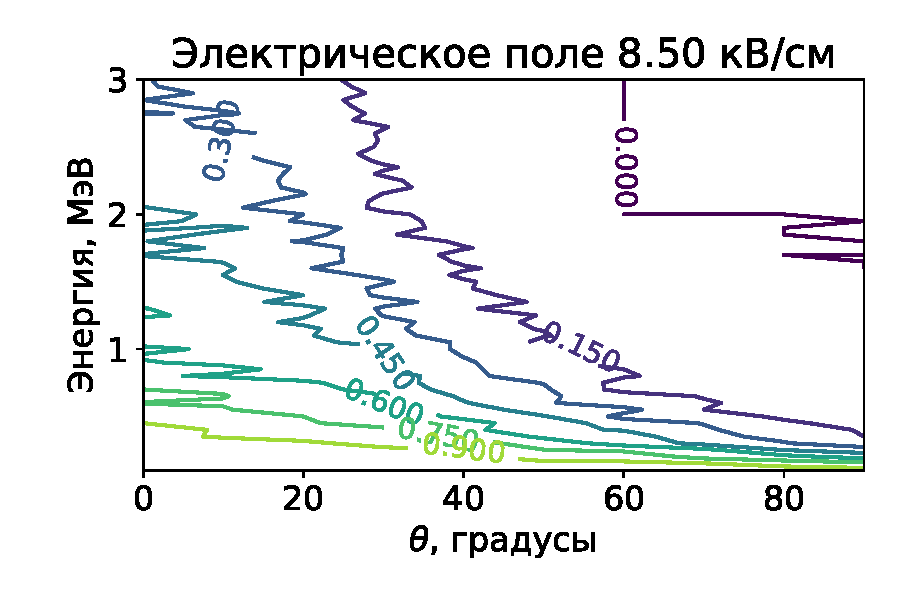
\includegraphics[width=\linewidth]{thunderstorm/rdfm/reverse_8_50.pdf} \\ з)}
        \end{minipage}    
        \vfill
        \begin{minipage}[h]{0.49\linewidth}
            \center{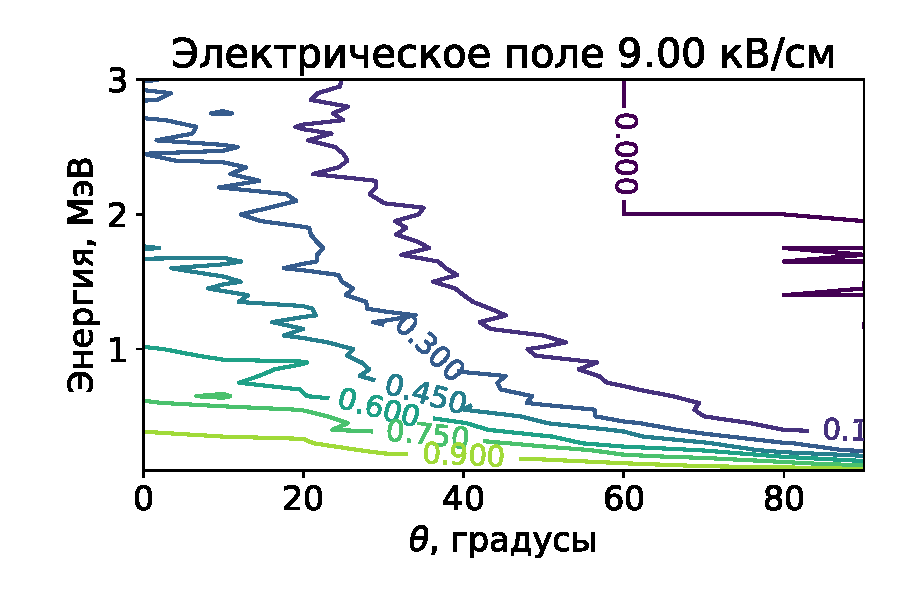
\includegraphics[width=\linewidth]{thunderstorm/rdfm/reverse_9_00.pdf} \\ и)}
        \end{minipage}
        \hfill
        \begin{minipage}[h]{0.49\linewidth}
            \center{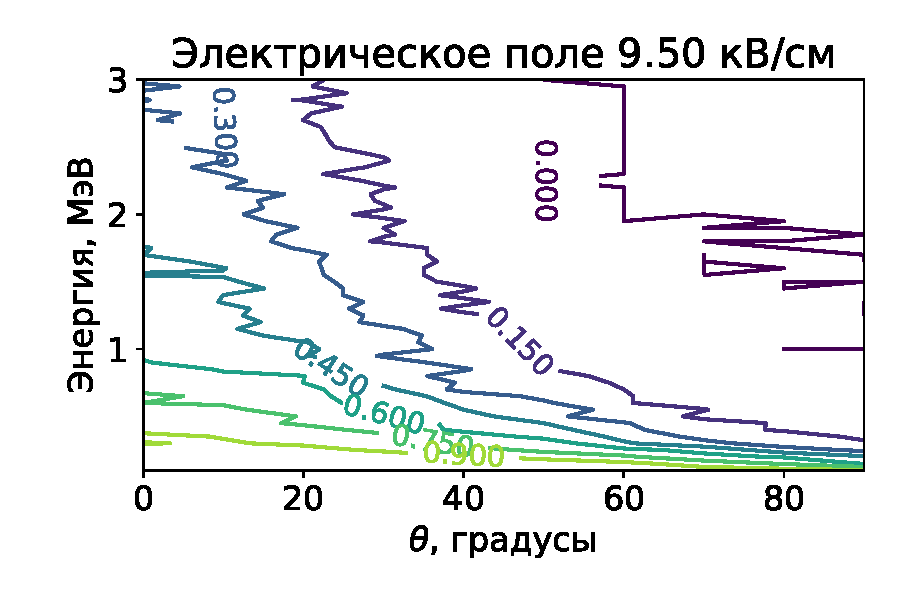
\includegraphics[width=\linewidth]{thunderstorm/rdfm/reverse_9_50.pdf} \\ к)}
        \end{minipage} 
        \vfill
        \begin{minipage}[h]{0.49\linewidth}
            \center{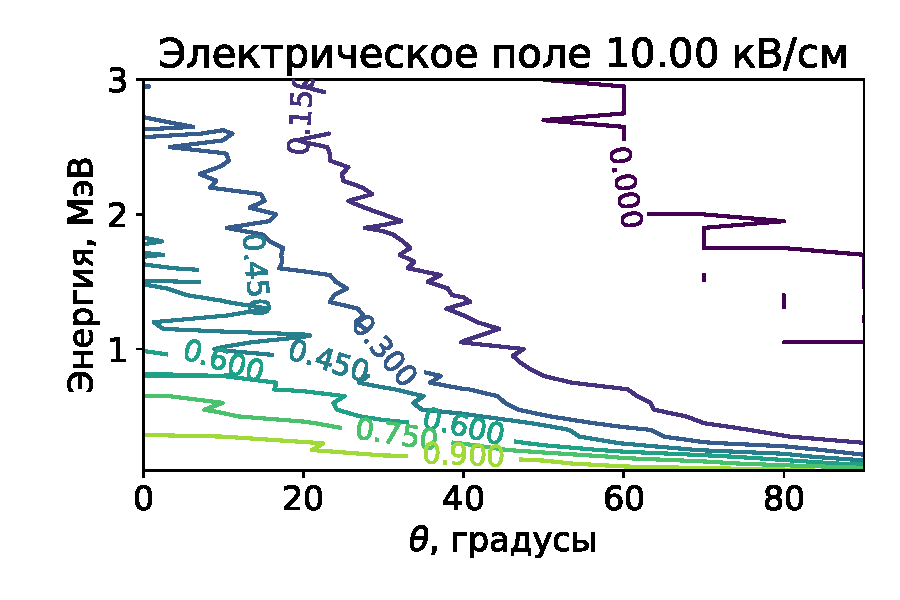
\includegraphics[width=\linewidth]{thunderstorm/rdfm/reverse_10_00.pdf} \\ л)}
        \end{minipage}
        \caption{Разворот электрона TODO(Скопировать)}
    \end{center}
    \label{fig:storm:reverse_nc_2}
\end{figure}


\begin{figure}[ph!]
    \begin{center}
        \begin{minipage}[h]{0.49\linewidth}
            \center{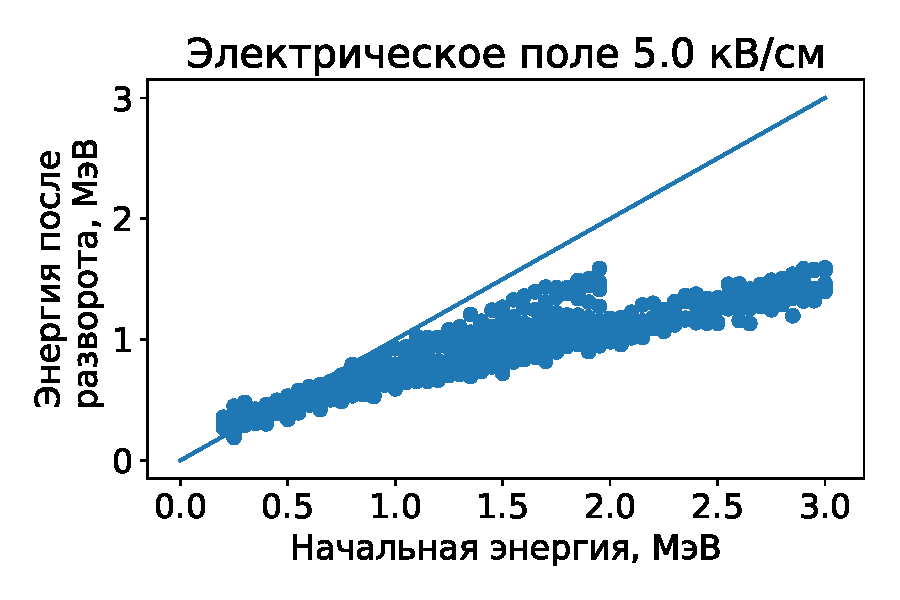
\includegraphics[width=\linewidth]{thunderstorm/rdfm/reverse_energy_5_0.pdf} \\ а)}
        \end{minipage}
        \hfill
        \begin{minipage}[h]{0.49\linewidth}
            \center{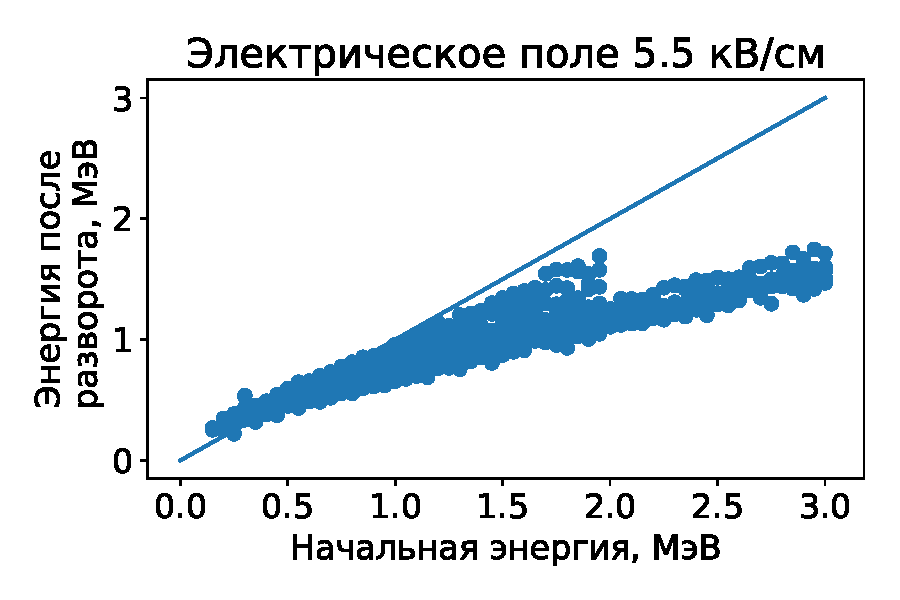
\includegraphics[width=\linewidth]{thunderstorm/rdfm/reverse_energy_5_5.pdf} \\ б)}
        \end{minipage}
        \vfill
        \begin{minipage}[h]{0.49\linewidth}
            \center{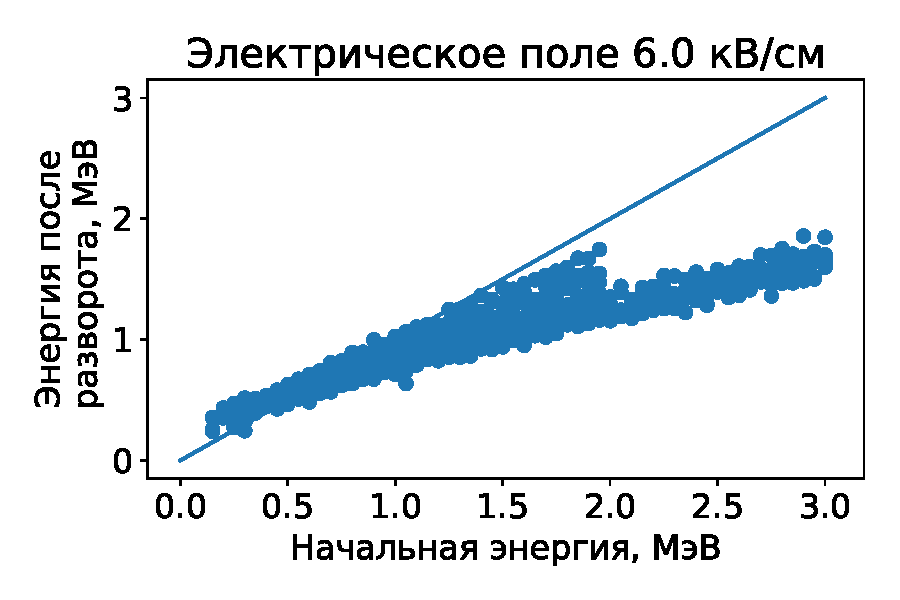
\includegraphics[width=\linewidth]{thunderstorm/rdfm/reverse_energy_6_0.pdf} \\ в)}
        \end{minipage}
        \hfill
        \begin{minipage}[h]{0.49\linewidth}
            \center{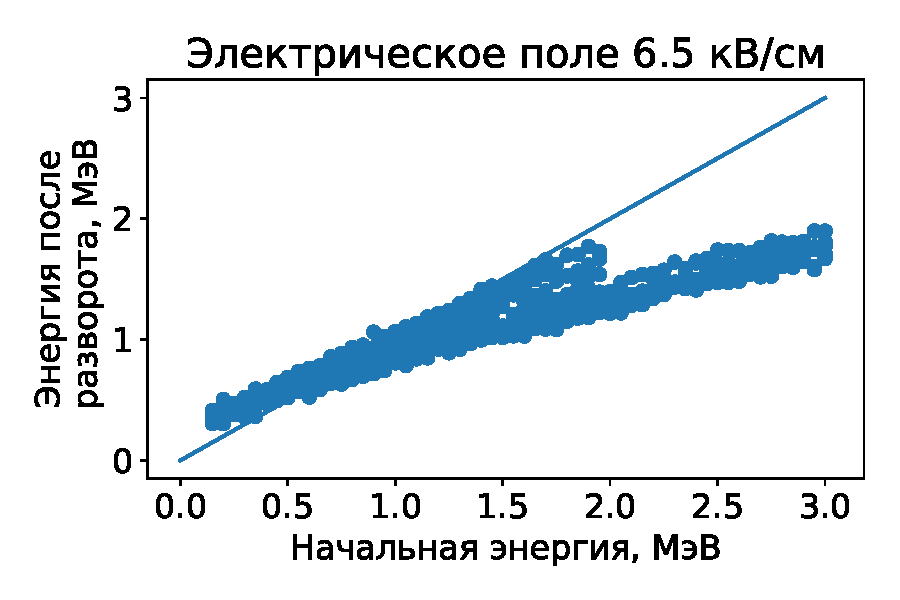
\includegraphics[width=\linewidth]{thunderstorm/rdfm/reverse_energy_6_5.pdf} \\ г)}
        \end{minipage}
        \vfill
        \begin{minipage}[h]{0.49\linewidth}
            \center{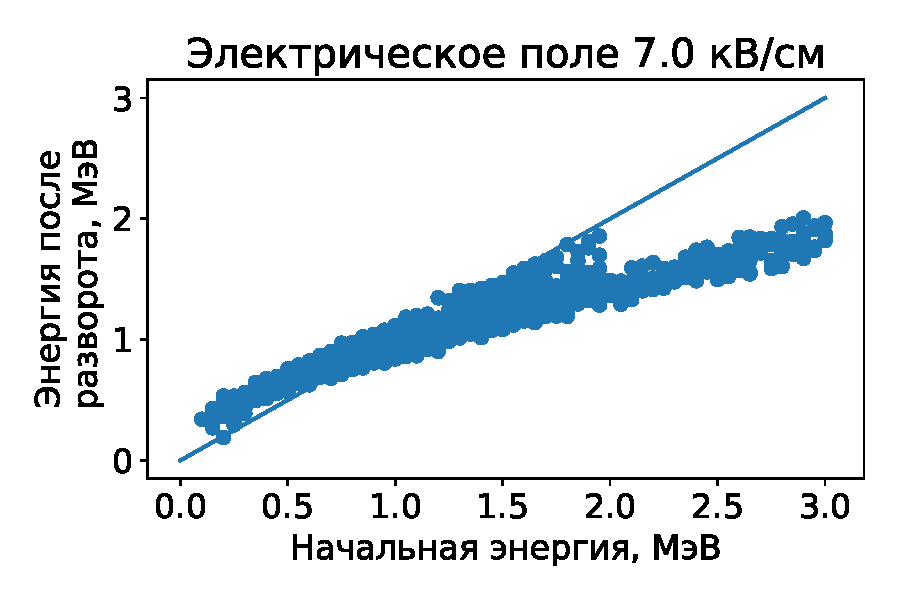
\includegraphics[width=\linewidth]{thunderstorm/rdfm/reverse_energy_7_0.pdf} \\ д)}
        \end{minipage}
        \hfill
        \begin{minipage}[h]{0.49\linewidth}
            \center{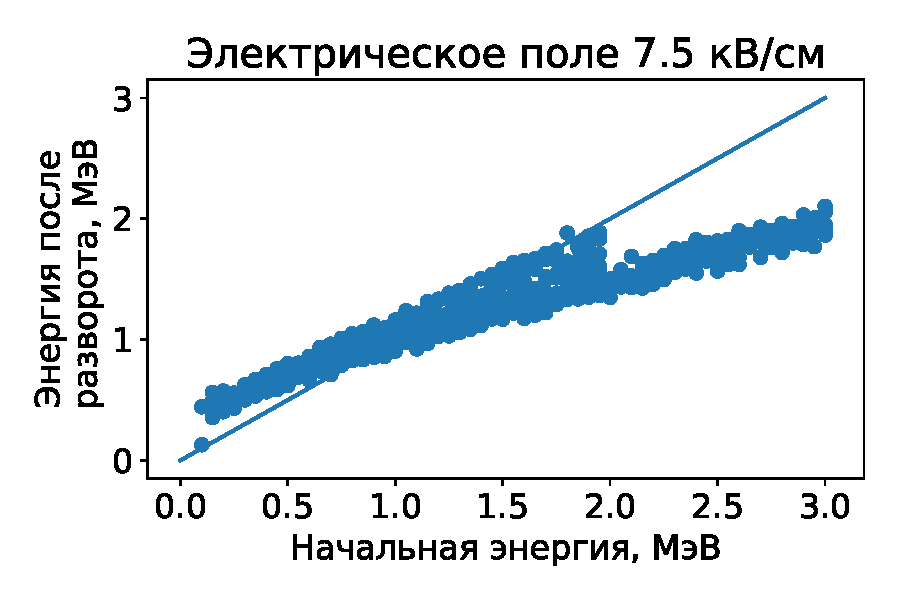
\includegraphics[width=\linewidth]{thunderstorm/rdfm/reverse_energy_7_5.pdf} \\ е)}
        \end{minipage}
        \caption{Зависимость средней энергии электрона после разворота от начальной энергии для разных значений электрического поля.}
    \end{center}
    \label{fig:storm:reverse_energy_nc_1}
\end{figure}
\begin{figure}[ph!]
    \begin{center}
        \begin{minipage}[h]{0.49\linewidth}
            \center{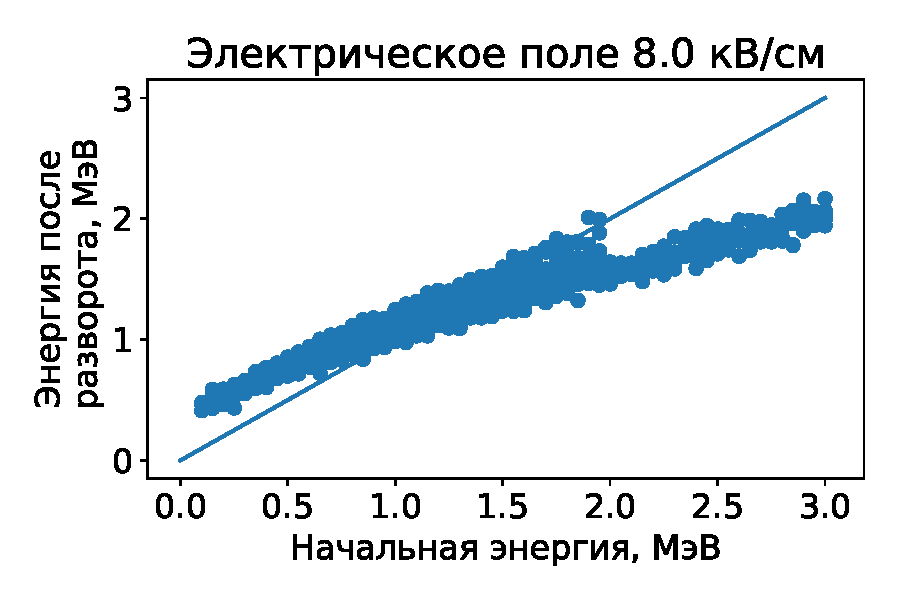
\includegraphics[width=\linewidth]{thunderstorm/rdfm/reverse_energy_8_0.pdf} \\ ж)}
        \end{minipage}
        \hfill
        \begin{minipage}[h]{0.49\linewidth}
            \center{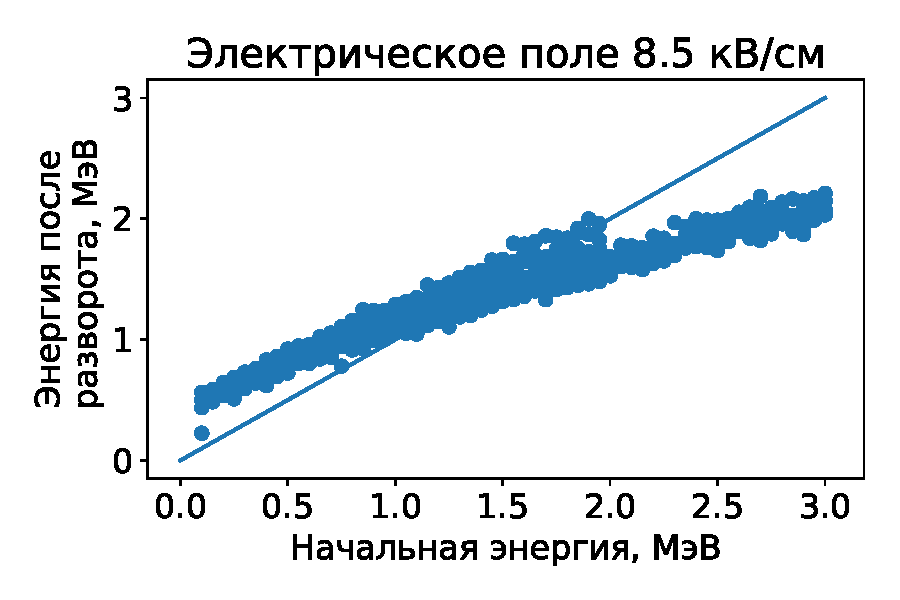
\includegraphics[width=\linewidth]{thunderstorm/rdfm/reverse_energy_8_5.pdf} \\ з)}
        \end{minipage}    
        \vfill
        \begin{minipage}[h]{0.49\linewidth}
            \center{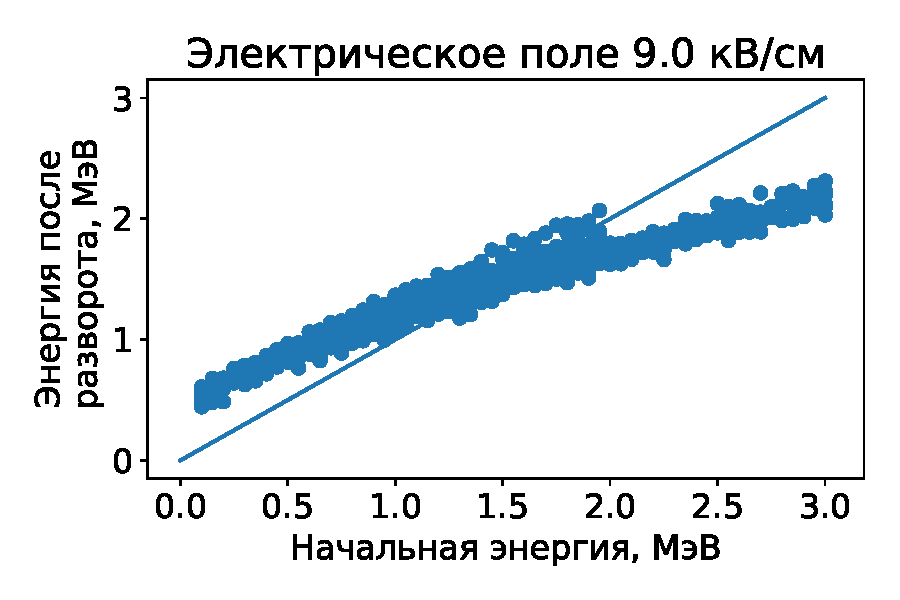
\includegraphics[width=\linewidth]{thunderstorm/rdfm/reverse_energy_9_0.pdf} \\ и)}
        \end{minipage}
        \hfill
        \begin{minipage}[h]{0.49\linewidth}
            \center{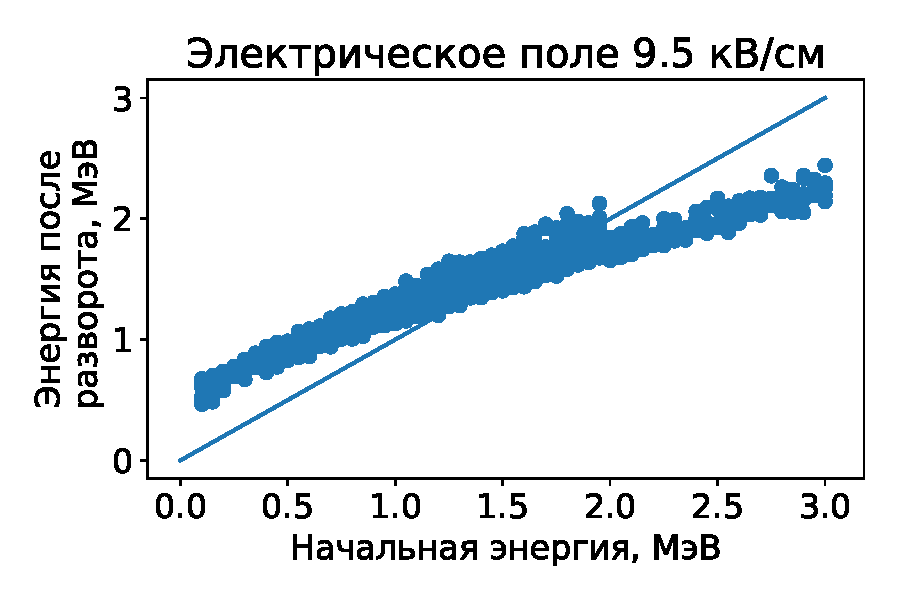
\includegraphics[width=\linewidth]{thunderstorm/rdfm/reverse_energy_9_5.pdf} \\ к)}
        \end{minipage} 
        \vfill
        \begin{minipage}[h]{0.49\linewidth}
            \center{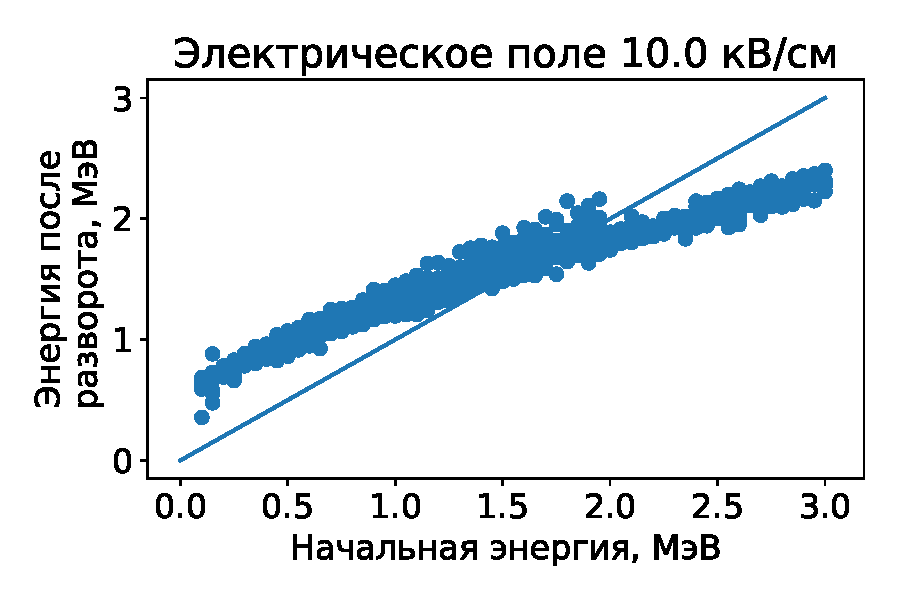
\includegraphics[width=\linewidth]{thunderstorm/rdfm/reverse_energy_10_0.pdf} \\ л)}
        \end{minipage}
        \caption{Зависимость средней энергии электрона после разворота от начальной энергии для разных значений электрического поля.}
    \end{center}
    \label{fig:storm:reverse_energy_nc_2}
\end{figure}
Далее было проведено моделирование рождения новых затравочных электронов, для этого было взято несколько точек вдоль и чуть выше кривой полученной Дуайером (отмечены на графике~\ref{fig:storm:dwyer2003}а красными треугольниками), и для данных точек было сделано GEANT4 моделирование лавины убегающих электронов.  Для каждой точки было рассчитано число новых затравочных электронов рожденных с помощью позитронов и гамма-квантов с учетом вероятности развернутся в электрическом поле, результаты представлены в таблице~\ref{tab:storm:dwyer}. Из проведенного моделирования можно сделать следующие выводы:
\begin{itemize}
	\item Результаты моделирования согласуются с результатами Дуаера, однако в отличии от него мы получили не просто качественную оценку наличия/отсутствия новых затравочных частиц, но и получили количественные оценки, также далее мы проведем структурный анализ новых затравочных электронов и покажем некоторые проблемы которые могут значительно уменьшать эффективность работы механизмов обратной связи.
	\item Наша количественная оценка позволяет сделать интересное наблюдение: на эффективность работы механизмов обратной связи в большей степени влияет длинна области с полем, чем величина поля. Это важный результат так как он говорит о проблемах стримерной гипотезы возникновения TGF, подробнее см раздел TODO(Раздел). 
\end{itemize}

\begin{figure}[t]
    \begin{center}
        \begin{minipage}[h]{0.49\linewidth}
            \center{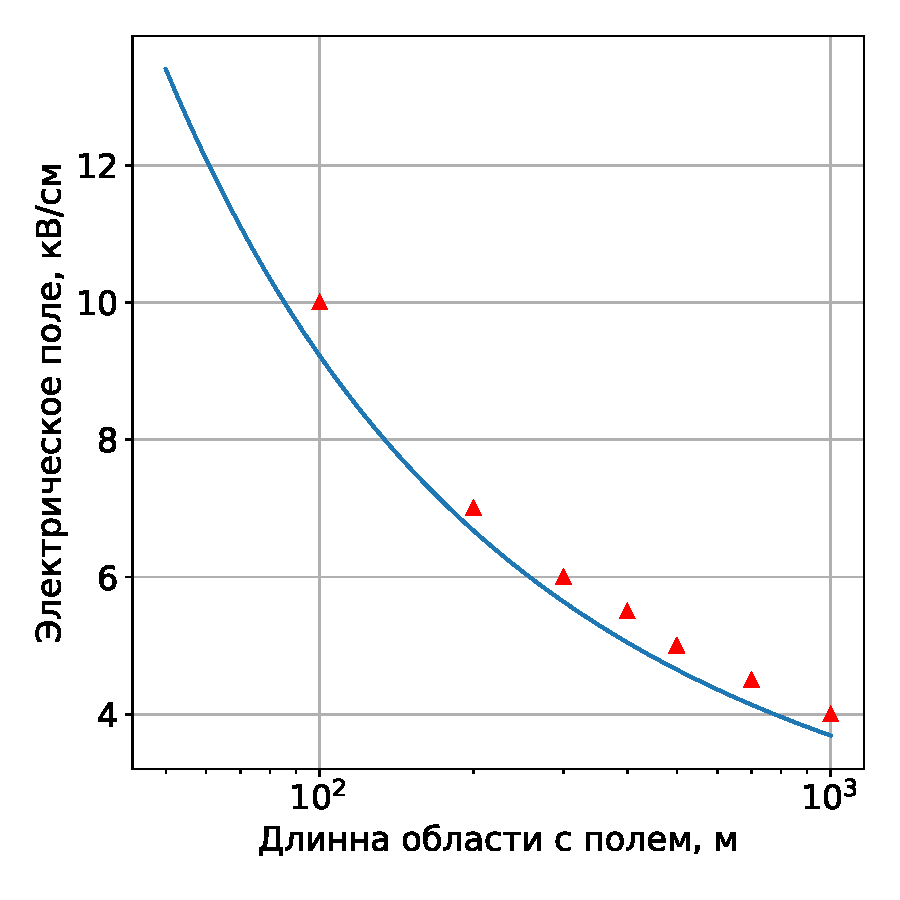
\includegraphics[width=\linewidth]{thunderstorm/rdfm/dwyer_2003.pdf} \\ а)}
        \end{minipage}
        \hfill
        \begin{minipage}[h]{0.49\linewidth}
            \center{\includegraphics[width=\linewidth]{thunderstorm/epl2020/radial-eps-converted-to.pdf}   \\ б)}
        \end{minipage}
        \caption{а) Затухание лавины. б) placeholder.}
    \end{center}
    \label{fig:storm:dwyer2003}
\end{figure}

\begin{table}[h]
    \centering
    \begin{tabular}{crrrr}
        \hline
        & & & \multicolumn{2}{r}{Число новых затравочных электронов} \\
        & Поле, кВ/см &  Длина облака, м  & от гамма ОС & от позитронной ОС \\
        \hline
        & 4   &  1000&  0 & 0  \\
        & 4.5 &  700 &  200 ($\pm 10 \%$)& 400 ($\pm 5 \%$) \\
        & 5   &  500 &  100 ($\pm 14 \%$)& 40 ($\pm 5 \%$) \\
        & 5.5 &  400 &  110 ($\pm 3 \%$)& 85 ($\pm 5 \%$) \\
        & 6   &  300 &  40 ($\pm 3 \%$)& 70 ($\pm 2 \%$) \\
        & 7   &  200 &  7 ($\pm 2 \%$)& 8 ($\pm 2 \%$) \\
        & 10  &  100 &  5 ($\pm 3 \%$)& 2 ($\pm 5 \%$) \\
        \hline
    \end{tabular}
    \caption{Моделирование числа новых затравочных электронов возникающих за счет одной итерации механизма обратной связи на один первичный электрон.}
    \label{tab:storm:dwyer}
\end{table}

Однако не смотря на то что наши результат совпали с результатами Дуайера, у его модели обратной связи можно отметить несколько недостатков. 

Моделирование Дуайера проводилось при нормальных условиях, то есть для атмосферы лежащей на уровне моря, однако реальные явления происходят больших высотах (например, на научных станциях на г. Арагац и на Тянь Шане производится наблюдение за грозовыми облаками идущими на высотах 3-5 километра, а спутниковые наблюдения говорят об источниках TGF расположенных на высотах 12-15 километров). Можно провести экстраполяцию от нормальных условий к условиям на больших высотах, считая что величины (такие как критическое  поле или поле для возникновения обратной связи) уменьшаются пропорционально плотности, а расстояния увеличиваются пропорционально плотности, как было предложен Дуайером, однако такие предположения имеет ограниченную точность. Например, проведенный в разделе ~\ref{sec:thunderstorm/rrea} расчет характерной длинны нарастания лавины был проведен при условиях соответствующей 10 километровой высоте и сравнивался с величиной полученной Дуайером, которая была рассчитана при нормальных условиях и экстраполирована к условия высота 10 км, полученные результат отличаются, хоть они и не дают такого различия как результаты полученные в работе~\cite{oreshkin2018}, но в рамках сравнения наших моделирований отличие существенно и может свидетельствовать он не правомерности интерполяции результатов полученных при нормальных условиях к условиях на больших высотах. 

Другим недостатком расчетов Дуайера является пренебрежение реальными размерами облака, для примера рассмотрим радиальное распределение рождения убегающих электронов показанное на рис.~\ref{fig:storm:dwyer2003}б, которое соответствует облаку на высоте 10 км. Видно, что электроны имеют широкое горизонтальное распределение которое может быть сравнимым с размером небольшого облака. Дополнительно следует учесть что фотоны могут переносить вторичные лавины далеко от начальных, или активно покидать облако. Если построить радиальные распределения рожденных новых затравочных электронов для точек из таблицы~\ref{tab:storm:dwyer}, то можно у видеть что для них также характерен широкий (более 500 метров) разброс, таким образом для облака с характерным размером порядка 1 километра, частицы уже во время второй или третей итерации обратной связи будут покидать облако и перестанут ускорятся. 
\begin{figure}[t]
    \begin{center}
        \begin{minipage}[h]{0.49\linewidth}
            \center{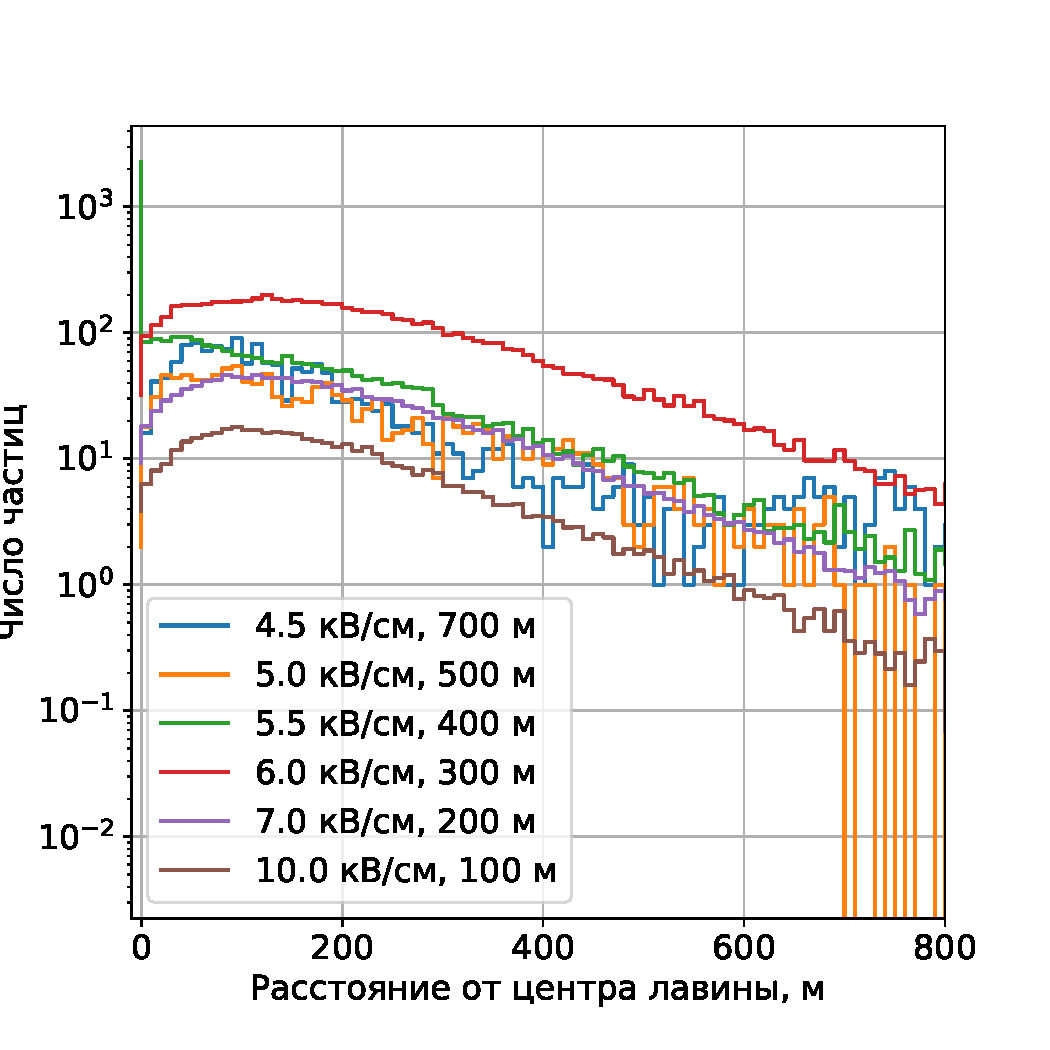
\includegraphics[width=\linewidth]{thunderstorm/rdfm/radial_gamma.pdf} \\ а)}
        \end{minipage}
        \hfill
        \begin{minipage}[h]{0.49\linewidth}
            \center{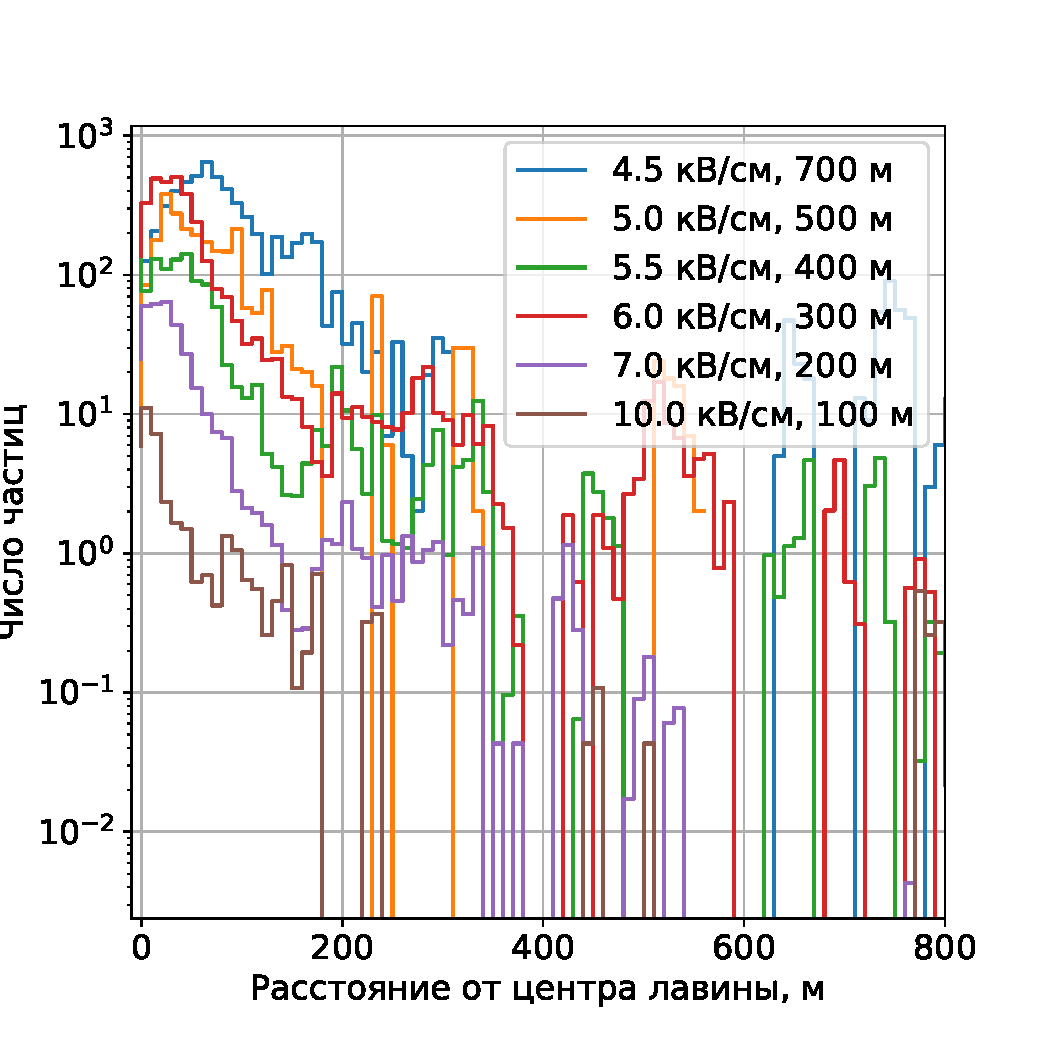
\includegraphics[width=\linewidth]{thunderstorm/rdfm/radial_positron.pdf}   \\ б)}
        \end{minipage}
        \caption{Радиальное распределение затравочных электронов рожденных за счет а) гамма обратной связи б) позитронной обратной связи.}
    \end{center}
    \label{fig:storm:radial_fb}
\end{figure}


Так важно учесть не только распределение в горизонтальном пространстве, но и по вертикали. Обычно в моделировании мы размещаем затравочную частицу в начале области с электрическим полем, однако новые затравочные частицы рождаемые за счет гамма или позитронной обратной связи имеют некоторое распределение по вертикали,  и поэтому для новой затравочной частицы длинна области с поле будет эффективно сокращаться по сравнению с длинной облака для первой затравочной частицы. Попробуем оценить как влияет это сокращение на работу механизмов обратной связи. Пусть расстояние от центра облака до его верхнего края равно $H$, именно в этой части рождаются новые затравочные частицы, разобьем это пространство на $N$ слоёв толщиной $\Delta h$, и подсчитаем с учетом вероятности разворота число $n(i)$ новых затравочных частиц на одну первичную частицу в $i$-том слое. Чтобы упростить расчеты и не учитывать влияние значения энергии и направления импульса частиц будем считать что все новые частицы могут порождать новые лавины также эффективно как первичная частица. Частицы расположенные в самом верхнем $N$-том слое считаются тождественными начальной частицы и если считать что на $j$-ой итерации в этом слое находится $k(N)^j$ частиц, то тогда на каждой итерации эти частицу будут создавать $n(i)*k(N)^j$ частиц в $i$-том слое. С частицами из следующих слоев сложнее, для частиц расположенных в $N-1$ слое с одной стороны расстояние на котором происходит развитие лавины уменьшилось, с другой над этими частица появилась область с полем: когда мы рассматриваем затравочную частицу инжектированную в самый верх облака, мы игнорируем частицы рожденные выше её, так как там находится область без поля, теперь же появилась дополнительная область где гамма-кванты и позитроны могут создавать затравочные частицы. В нашей оценке трудно точным образом учесть эти факторы, но поскольку они имеют разную направленность и могут компенсировать друг друга, давайте рассмотрим такую модель:  будем рассматривать частицы как будто они инжектированы в верную часть объема и производят соответствующим образом распределенные затравочные частицы, однако будет брать из этого распределения только ту часть которая, ложится на границы между выбранным слоем и серединой облака. Иначе говоря мы будет считать что если в некотором слое $l$ на $j$-ой итерации содержится $k(l)^j$ частиц, то они будут генерировать затравочные частицы только в слоях от первого до $l$-ого включительно, причем число сгенированных частиц в  $i$-том слое будет равно $k(l)^j * n(i+N-l)$. Теперь можно посчитать сколько частиц генерируется в слое за одну итерацию:
\begin{equation}
P(i)^{j} = \sum_{l=i}^{N} k(l)^j * n(i+N-l)
\end{equation}
Приведенный код на языке Python позволяет вычислить число частиц для заданной итерации:
\begin{lstlisting}[language=Python]
import numpy as np

def feedback(distrubution : np.ndarray, max_iteration: int) -> np.ndarray:
    distrubution = distrubution[::-1]
    for i in range(max_iteration):
        temp = np.zeros(distrubution.size)
        for indx, it in enumerate(distrubution):
            if indx == 0:
                temp = it*distrubution
            else:
                temp[indx:] += it*distrubution[:-indx]
        distrubution = temp
    return distrubution
\end{lstlisting}
Данная функция принимает в качестве аргумента \textit{distrubution} массив значений $n(i)$ для каждого слоя, а аргумент \textit{max\_iteration} задает итерацию для которой вычисляется конечное число частиц. На графике приведены количество частиц на разных итерация обратной связи для нескольких симуляций с разными значения электрического поля и длинны облака, величина $\Delta h$ во всех симуляциях взята равной 10 метрам. 

Рассмотрим результаты моделирования: в двух случаях мы видим гигантский рост частиц как и предсказывает Дуайер, однако в трех других случаях обратная связь затухает --- сказывается недостаток частиц в верхней частиц облака. Отсюда можно сделать несколько выводов: 
\begin{itemize}
    \item Полученных Дуаером условий может быть недостаточным для возникновения обратной связи, параметры определенные им в работе ~\cite{} могут быть не достаточны, и требуется увеличение электрического поля, однако при увеличении поля свыше 10 кВ/см мы попадем в область где уже становится возможным возникновения обычного электрического пробоя, и потому рассмотрение пробоя на убегающих электронов становится избыточным;
    \item Подтверждается тезис о том что увеличение длинны облака эффективнее чем усиление поля;
    \item Исходя из предыдущего пункта можно оспорить тезис Дуаера о том что механизмы обратной связи позволяют опровергнуть гипотезу о наличии скрытых внутриоблачным областей с сильным полем, как мы видим из моделирования как раз для такого случая (малый размер, сильное поле) механизмы обратной связи быстро затухают из-за смещения точки рождения затравочных частиц от верхнего края облака;
\end{itemize}

\begin{figure}[ph!]
    \begin{center}
        \begin{minipage}[h]{0.49\linewidth}
            \center{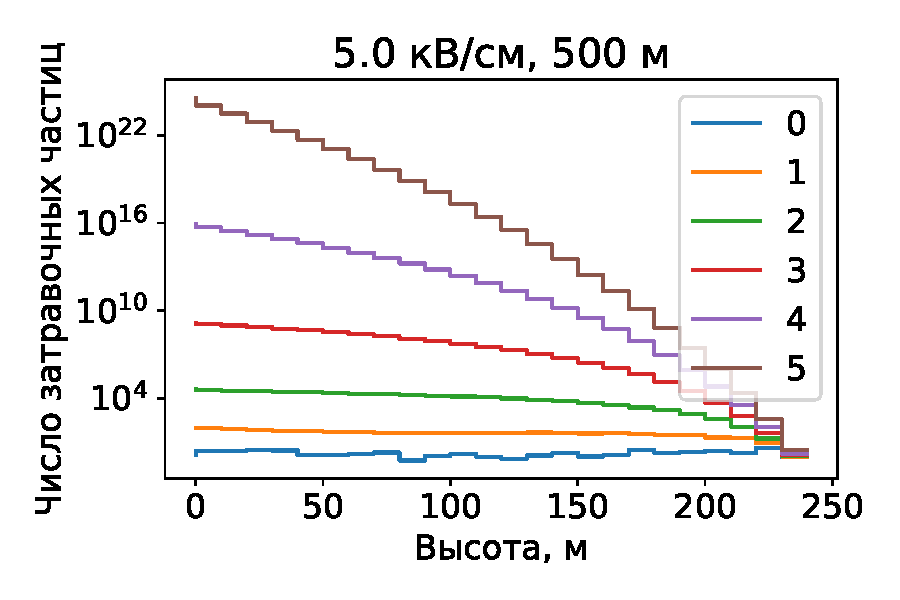
\includegraphics[width=\linewidth]{thunderstorm/rdfm/vertical_gamma_5_0.pdf} \\ а)}
        \end{minipage}
        \hfill
        \begin{minipage}[h]{0.49\linewidth}
            \center{\includegraphics[width=\linewidth]{thunderstorm/rdfm/vertical_gamma_5_5.pdf} \\ б)}
        \end{minipage}
        \vfill
        \begin{minipage}[h]{0.49\linewidth}
            \center{\includegraphics[width=\linewidth]{thunderstorm/rdfm/vertical_gamma_6_0.pdf} \\ в)}
        \end{minipage}
        \hfill
        \begin{minipage}[h]{0.49\linewidth}
            \center{\includegraphics[width=\linewidth]{thunderstorm/rdfm/vertical_gamma_7_0.pdf} \\ г)}
        \end{minipage}
        \vfill
        \begin{minipage}[h]{0.49\linewidth}
            \center{\includegraphics[width=\linewidth]{thunderstorm/rdfm/vertical_gamma_10_0.pdf} \\ д)}
        \end{minipage}
        \caption{Моделирование гамма обратной связи для различных облаков, на графиках приведено распределенное по высоте число частиц, на различных итерациях обратной связи, нулевая итерация соответствует частицам рожденным первичной затравочной частицей.}
    \end{center}
    \label{fig:storm:vertical_gamma}
\end{figure}
\begin{figure}[ph!]
    \begin{center}
        \begin{minipage}[h]{0.49\linewidth}
            \center{\includegraphics[width=\linewidth]{thunderstorm/rdfm/vertical_positron_5_0.pdf} \\ а)}
        \end{minipage}
        \hfill
        \begin{minipage}[h]{0.49\linewidth}
            \center{\includegraphics[width=\linewidth]{thunderstorm/rdfm/vertical_positron_5_5.pdf} \\ б)}
        \end{minipage}
        \vfill
        \begin{minipage}[h]{0.49\linewidth}
            \center{\includegraphics[width=\linewidth]{thunderstorm/rdfm/vertical_positron_6_0.pdf} \\ в)}
        \end{minipage}
        \hfill
        \begin{minipage}[h]{0.49\linewidth}
            \center{\includegraphics[width=\linewidth]{thunderstorm/rdfm/vertical_positron_7_0.pdf} \\ г)}
        \end{minipage}
        \vfill
        \begin{minipage}[h]{0.49\linewidth}
            \center{\includegraphics[width=\linewidth]{thunderstorm/rdfm/vertical_positron_10_0.pdf} \\ д)}
        \end{minipage}
        \caption{Моделирование позитронной обратной связи для различных облаков, на графиках приведено распределенное по высоте число частиц, на различных итерациях обратной связи, нулевая итерация соответствует частицам рожденным первичной затравочной частицей.}
    \end{center}
    \label{fig:storm:vertical_gamma}
\end{figure}

Пока мы следуя работе Дуайера проводили моделирование при нормальных условиях, однако как уже отмечалось не совсем корректно экстраполировать эти результаты на большие высоты. Поэтому в данной работе мы рассмотрим моделирование на больших высотах, соответствующее более реалистичным условиям, а именно возьмем плотность воздуха 0.5 кг/м$^3$, что примерно соответствует высоте в 8 километров, реалистичные значения электрического поля в атмосфере не превышают 2.25 кВ/см, поэтому мы возьмем для моделирования диапазон значение от 1 до 2.25 кВ/см, так же мы наложим ограничения на размер облака, оно будет представлять собой куб со стороной 400 метров. На основе данного моделирования рассчитан коэффициенты гамма и позитронной обратной связи (при подсчете затравочных электронов, также как и раннее учитывалась возможность разворота, смотри рисунок~\ref{fig:storm:ayss2018}а), зависимость которых от поля отображена на рисунке~\ref{fig:storm:ayss2018}б. Как мы видим даже в самом оптимистичном сценарии вклад обратной связи в рост числа электронов в лавине не превышает 10~\%. Методика и результаты этого моделирования представлены в работе~\cite{antidwyer} 

\begin{figure}[t]
    \begin{center}
        \begin{minipage}[h]{0.49\linewidth}
            \center{\includegraphics[width=\linewidth]{thunderstorm/ayss_2018_rev.pdf} \\ а)}
        \end{minipage}
        \hfill
        \begin{minipage}[h]{0.49\linewidth}
            \center{\includegraphics[width=\linewidth]{thunderstorm/ayss_2018_fb.pdf}   \\ б)}
        \end{minipage}
        \caption{а) Предельный угол между направление движения электрона и электрическим полем при котором происходит разворот электрона. б)Коэффициент гамма и позитронной обратной связи для следующих параметров: энергия затравочного электрона --- 3 МэВ, размер области с полем --- 400 метров, плотность воздуха --- 0.5 кг/м$^3$ ($\sim 0.5$ атм).}
    \end{center}
    \label{fig:storm:ayss2018}
\end{figure}
Подводя итоги этого раздела можно сказать что не смотря на то что по результатам моделирования проведенного в разделе~\ref{sec:thunderstorm/rrea}, учет гамма-квантов и позитронов необходим, достоверно утверждать что они могут запускать механизм приводящие к взрывному числа частиц нельзя, что подтверждается рядом экспериментальных наблюдений (TODO(ссылка на Чилингаряна)) 
\section{Анализ структуры грозового облака на основе наблюдения TGE}\label{sec:thunderstorm/llletge} 
В отличии от TGF представляющие собой очень короткие (~10 мкс) вспышки гамма- и рентгеновского излучения из грозового облака, TGE представляет собой длительное повышение гамма-фона. По результатам наблюдений на горе Арагац академиком Чилингаряном была предложено разделить TGE на две условные группы: 
High Energy Particle TGE (HEP TGE) имеющие длительность порядка нескольких минут и значительную высокоэнергичную (энергия гамма-квантов более 3 МэВ) компоненту и Long-Lasting Low Energy TGE (LLLL TGE) имеющие длительность более двух часов и при этом содержащие в основном низкоэнергитичные (менее 3 МэВ) гамма-кванты. При этом можно отметить следующие особенности: 
\begin{itemize}
    \item HEP TGE  возникает при глубоких  провалах  приповерхностного поля, но не каждый провал сопровождается HEP TGE,
    \item Возможно существование LLLE TGE без  HEP TGE,
    \item Возможно cуществование LLLE TGE при полях ниже поля убегания электронов,
    \item HEP TGE может возникать несколько раз: оно может быть разрушено из-за вспышки молнии и потом восстановится.
\end{itemize}
В контексте изучения возникновения молнии HEP TGE и LLLE TGE интересны, так как они могут помочь описать структуру грозового облака.  Так первым представление об грозовом облаке был вертикальный диполь, однако реальная его структура гораздо сложнее, в данной работе мы рассмотрим генерацию TGE c точки зрения трипольной модели(хотя по всей видимости облака могут иметь и большее число слоев). При представлении облака как вертикального триполя считается что в центре облака собирается отрицательный заряд, в верхней части облака и на земле индуцируется положительный заряд, и наконец в нижней части облака формируется небольшая область с положительным зарядом. Тогда можно сформулировать следующие гипотезы:
\begin{itemize}
    \item Затравочными частицами служат электроны от космических лучей;
    \item LLLE TGE -возникает за счет поля между основным отрицательным зарядом и зарядом индуцированным в земле;
    \item По мере развития нижнего положительного заряда (НПЗ)  возрастает поле и поток частиц в LLLE TGE переходит в HEP TGE;
    \item Регистрация HEP TGE происходит при прохождении НПЗ над детектором
\end{itemize}
Для проверки этих гипотез в работе были проанализированны экспериментальные наблюдения которые сравнивались с моделированием с помошью CORSIKA и GEANT4. Далее приводятся результаты проведенного для этой работы  автором диссертации GEANT4 моделирования. В частности автором были проведенным моделирования превышения гамма-квантов в зависимости от электрического поля, а также получены их угловые и радиальные распределения. Симуляция проводилась при следующих параметрах: первичными частиц являются гамма-кванты в диапазоне энергий от 1 до 100 МэВ, имеющие степенной спектр вида $E^{-1.42}$, начальная точка расположена в тысяче метрах над станцией(которая находится на высоте 3200 метров над уровнем моря), моделирование проводилось в подкритических полях (значение критического поля для данных высот порядка 1.7-1.8 кВ/см
), также моделирование проводилось с использование двух физических листов G4EmPhysStandard и G4EmPhysStandar\_opt4 (использовался GEANT4 версии 4.10.4). График демонстрирует рост потока гамму, даже в подкритических полях и взрывной рост при приближении к порогу. Левый график демонстрирует радиальное расхождение гамма-квантов от RREA вследствии комптон-эффекта, как мы видим маловероятно наблюдать гамма-кванты на растоянии большем километра от центра лавины, кроме того для гамма-квантов рассеявшихся на растояние более километра, максимум по углу смещен в горизонтальный сторону, что затрудняет их регистрацию. Результаты моделирования автора согласуются с другим моделированием проведенным в программе CORSIKA, и на основе анализа приведенного в работе можно утверждать что сформулированные гипотезы выполняются и можно сделать вывод что наблюдаемые данные по TGE могут быть объяснены трипольной структурой облака поля и наблюдение за TGE можно использовать для наблюдения эволюции нижнего заряженного слоя, его образования, перемещения и разрушения.  

\section{Нейтроны в грозовых облаках}\label{sec:thunderstorm/neutron} 

Ещё одним интересным следствием из феномена убегающих электронов является наличие нейтронного излучение из грозового облака. Действительно так энергиях гамма-квантов в явлениях TGF и TGE может достигать десятков мегаэлектрон-вольт то становится возможным прохождение фотоядерных реакций, генерирующих поток нейтронов. Это следствие находит экспериментальные наблюдения, например исследование на научной станции на Тянь-Шане сначала регистрировали понижение потока нейтронов по время грозовой активности [], но в более поздней работе отмечают регистрацию значительного роста потока нейтронов. Также повышение потока нейтронов подтверждаются наблюдения на научной станции на г. Арагац. Есть определенные вопрос к источнику нейтронов, ряд исследователей полагаю что повышение потока нейтронов обусловлено не проходящими в облаке фотоядерным реакциями, а обусловлено другими источниками, например вымыванием радиоактивных элементов из почвы во время дождя и выходом радона, но исследования в работе опровергают эту гипотезу.
% Статья Antonova-2009.pdf - Установлено, что прохождение грозовых облаков над высотной станцией снижает скорость счета штатного нейтронного монитора на ~ 1.2% относительно уровня ясной погоды (при положительных электрических полях 40–50 кВ м –1). Влияние вариаций электрического поля проявляется в низкоэнергетической части спектра нейтронов и отсутствует в высокоэнергетической (множественность эмиссии нейтронов превышает 6). Обнаруженный нами эффект не случаен; он имеет более высокие пороговые значения энергии и величины для высотной станции по сравнению с прогнозируемыми значениями. Существенных изменений скорости счета монитора при скачках поля, вызванных грозовыми разрядами, не обнаружено. 
% Gurevich_Phys_Rev_Lett_2012.pdf - Мы впервые сообщаем здесь о регистрации необычайно высокого потока нейтронов низкой энергии, генерируемого во время гроз. Измеренные увеличения скорости счета нейтронов напрямую связаны с грозовыми разрядами. Полученное в нашей работе значение потока низкоэнергетических нейтронов является проблемой для фотоядерного канала генерации нейтронов во время грозы: расчетное значение необходимого потока высокоэнергетических лучей примерно на 3 порядка выше наблюдаемого. 

Принимая гипотезу о том что повышение потока нейтронов связанно с происходящими в облаке высокоэнергетическими процессами, можно предположить что регистрация нейтронов может дать информацию о величине потока и энергетических характеристиках гамма-квантов в грозовом облаке. Поэтому в рамках проектирования орбитального детектора для проекта ЧИБИС был поднят вопрос о целесообразности размещения на спутнике детектора нейтронов. Для ответа на этот вопрос было проведено моделирование чтоб оценить потенциальный поток нейтронов который можно было бы измерить на орбите. В симуляциях запускались гамма-кванты двух энергий  (15 и 100 МэВ) с высоты 15 километров, и рассчитывалось распределение рождения нейтронов по высоте, определялись характеристики рожденных частиц, так же моделировалось рождение нейтронов в детекторе из полистирола. 

\begin{figure}[t]
    \begin{center}
        \begin{minipage}[h]{0.49\linewidth}
            \center{\includegraphics[width=\linewidth]{thunderstorm/neutron/air_z_15MeV.pdf} \\ а)}
        \end{minipage}
        \hfill
        \begin{minipage}[h]{0.49\linewidth}
            \center{\includegraphics[width=\linewidth]{thunderstorm/neutron/air_z_100MeV.pdf}   \\ б)}
        \end{minipage}
        \caption{Распределение рождения нейтронов по высоте для фотонов с начальной энергией а) 15 МэВ б) 100 МэВ. Нормировано на одну первичную частицу.}
    \end{center}
    \label{fig:storm:neutron_z}
\end{figure}

По результатам моделирования для гамма-квантов с начальной энергией 100 МэВ получено что рождается примерно 1,7 на тысячу гамма-квантов с энергией 100 МэВ. Примерно половина нейтронов имеет энергию до 10 МэВ, вторая часть имеет медленно спадающий спектр в диапазоне от 10 до 70 МэВ. Разброс при рождении в атмосфере достаточно мал, порядка 85 \% нейтронов рождаются в стволе пучка гамма-квантов. Направление импульса рожденных нейтронов имеет достаточно широкий разброс, не позволяющий говорить о наличии выделенного направления движения. График~\ref{fig:storm:neutron_z}а показывает распределение точек рождение нейтронов по высоте. Как мы видим нейтроны рождаются на высотах до 70 километров, далее атмосфера становится сильно разреженной для того что бы шанс с рождения нейтрона был достаточно значительный. Можно отметить что в атмосфере взаимодействует только порядка 0.4 \% гамма-квантов, остальные 99.6\% улетают в космос. Также следует учесть то что гамма-кванты могут рождать нейтроны столкнувшись с корпусом космического аппарата (КА) и телом детектора, однако как показало моделирование, даже если считать что все долетевшие до КА частицы взаимодействуют в нем (что вообще говоря невозможно так как требует КА с массо-габаритным характеристикам значительно превосходящими реальные аппараты), то число таких нейтронов будет составлять только 8\% от числа рожденных в атмосфере.

Результаты моделирования для гамма-квантов с начальной энергией 15 МэВ в целом аналогичны, число рожденных нейтронов примерно в три раза меньше чем для 100 МэВ гаммы, они рождаются на высотах до 40 км (график распределения по высоте приведена на рис.~\ref{fig:storm:neutron_z}б). Только 5\% таких гамма-квантов долетает до космоса, и они не выбывают нейтроны с детектора в КА. Вопрос о достижимости детектора на КА рожденными в атмосфере нейтронов  является дискуссионным, простое GEANT4 моделирование показывает достаточно быструю потерю энергии быстрыми нейтронами, однако есть сомнения в точности выбранной модели, также есть работы показывающий что при больших потоков гамма-квантов возможно достижение нейтронами высот больших 400 км (ссылка а чувака). Однако те не менее моделирование показывает что число нейтронов будет не значительным и размещение детектора нейтронов на КА является не целесообразным и гораздо более эффективным является работа по  регистрации непосредственно гамма-квантов которые долетают до КА в больших количествах.
  
\section{Reactor like TGE-model}\label{sec:thunderstorm/reactor}

Общим недостатком рассмотренных выше моделей является упрощенная модель электрического поля: оно считается однородным по величине и направлению, что очевидно не так и в полу должны присутствовать разного рода неоднородности, вызванные как краевыми эффектами, так и возникновением сложных конфигураций зарядов. Точное моделирование и анализ динамики лавин убегающих электронов представляет собой сложную задачу, поэтому рассмотрим упрощенную модель что бы оценить потенциальные результаты, которые могут принести исследования в данном направлении. 

Чем ситуация в неоднородном по направлению поле отличается от развития лавин в однородном поле? Когда поле однородно то если гамма-кванты рождают новые затравочные электроны, то лавины от этих электронов будут направлены в том же направлении что и  первая лавина, но при этом их вершина будет смещена к  краю облака, что будет постепенно приводить к затуханию (как показано в предыдущих главах). Если же поле неоднородно по направлению, то направление новых лавин зависит от локальной конфигурации поля и таким образом может возникнуть ситуация изображенная на рисунке --- гамма-кванты от первичной лавины "зажигают" новые локальные ускоряющие ячейки, которые генерирует гамма кванты с угловым распределение значительно развернутым относительно углового распределения исходной лавины, что способствует более равномерному распределению новых затравочных электронов по облаку и как следствие  самоподдерживающей генерации лавин убегающих электронов.
Что бы смоделировать этот процесс, мы рассмотрим такую модель:
\begin{itemize}
    \item Используем только один изменяемый параметр --- локальный коэффициент размножения гамма-квантов, который дает обобщенное описание состояние атмосферы (величины электрического поля, плотности воздуха, вероятности зажигания ячейки и. т. д.)
    \item  Пренебрежем значением энергии гамма-квантов, пробег гамма-квантов будем разыгрывать на основе экспоненциального распределения с фиксированной длинной свободного пробега, много меньшей размеров облака;
    \item Также мы будем считать что при взаимодействии он гарантированно зажигает ячейку (фактически вероятность зажечь ячейку мы спрятали в локальном коэффициенте размножения);
    \item При зажигании ячейки мы не моделируем прохождение электронной лавины, а сразу генерируем вторичные гамма-кванты, их количество разыгрывается с помощью распределения Пуассона с локальным коэффициентом размножения гамма-квантов в качестве среднего, направление движения рожденных гамма-квантов считается однонаправленным с направлением электрического поля в точке рождения;
    \item Электрическое поле генерируются случайным образом на основе положения электрических зарядов местоположения которых разыграны на основе гауссова случайного блуждания;
    \item Облако представляется в виде куба со стороной в один километр, частицы покинувшие облако перестают отслеживаться.
\end{itemize}

В результате моделирования можно выделить три сценария: 
\begin{itemize}
    \item При малых значения локального коэффициента размножения роста гамма-квантов не происходит и высокоэнергетические процессы быстро затухают;
    \item При локальном коэффициенте размножения равным примерно 1.7 становится возможным медленное нарастание числа гамма-квантов, которое приводит к относительно стабильному самоподдерживающийся процессу, который однако с течением времени все же затухает. В целом этот сценарий хорошо описывает TGE-подобные явления;
    \item При превышении локальным коэффициентом размножения значения 1.8 происходит взрывной экспоненциальный рост числа гамма-квантов. Быстрый рост и большое количество гамма-квантов позволяет сказать что этот сценарий хорошо описывают TGF-подобные явления.
\end{itemize}

Для того чтобы проиллюстрировать эти три сценария, в работе приведены графики роста числа гамма-квантов в облаке от времени. Так график показывает затухание процессов при недостаточном значении локального коэффициента размножения, в данном примере несмотря на то что начальные гамма-кванты смогли сгенерировать некоторое количество вторичных частиц за время порядка 300 микросекунд все процессы затухли. График напротив показывает экспоненциальный рост за времена порядка 50-100 микросекунд (следует отметить что это согласуется со временем реально наблюдаемых TGF) при значения локального коэффициента размножения большего 1.8. Очень интересен график в нем наблюдается постепенный рост на достаточно большом (порядка 3 секунд) времени, что позволяет нам перейти от действующий на микровременных масштабах TGF к долговременным TGE. 

\begin{figure}
    \centering
    \begin{overpic}[scale=.5]{thunderstorm/rltge/electric_streams.pdf}
        \put(15,53){\includegraphics[scale=.015]{thunderstorm/rltge/cell.pdf}}
        \put(20,69){\text{Ускоряющая ячейка}}
        \put(10,10){\includegraphics[scale=.15]{thunderstorm/rltge/draw.pdf}}
    \end{overpic}
    \caption{
        Processes occurring in the RL-TGE model: gamma quanta run local acceleration processes in different parts of the cloud with a multidirectional electric field.
    }
    \label{fig:rl}
\end{figure}


\begin{figure}[t]
    \begin{center}
        \begin{minipage}[h]{0.49\linewidth}
            \center{\includegraphics[width=\linewidth]{thunderstorm/RL_proofTGE.pdf} \\ а)}
        \end{minipage}
        \hfill
        \begin{minipage}[h]{0.49\linewidth}
            \center{\includegraphics[width=\linewidth]{thunderstorm/RL_proofTGF.pdf}   \\ б)}
        \end{minipage}
        \caption{а) TGE-подобное нарастание. б) TGF-подобное нарастание.}
    \end{center}
    \label{thunder:rl_1}
\end{figure}


\begin{figure}[t]
    \begin{center}
        \begin{minipage}[h]{0.49\linewidth}
            \center{\includegraphics[width=\linewidth]{thunderstorm/RL_Extinction.pdf} \\ а)}
        \end{minipage}
        \hfill
        \begin{minipage}[h]{0.49\linewidth}
            \center{\includegraphics[width=\linewidth]{thunderstorm/RL_Extinction.pdf}   \\ б)}
        \end{minipage}
        \caption{а) Затухание лавины. б) placeholder.}
    \end{center}
    \label{thunder:rl_2}
\end{figure}

Характер высокоэнергичных процессов в облаке в нашей модели напоминает происходящее в ядерных реакторах, где изменение одного параметра (коэффициента размножения нейтронов приводит либо к затуханию реактора, либо к стабильной выработке энергии, либо к взрыву топлива), поэтому мы называем нашу модель атмосферным реактором, и так же по аналогии можем выделить подкритический и критический режим работы реактора. Критический режим соответствует активному размножению гамма-квантов, которые порождают все больше лавин убегающих электронов что приводит к активной ионизации объема облака. Подкритический режим соответствует значению коэффициента размножения  при котором с одной стороны процессы в облаке постоянно стартуют в следствии подпитки внешними КЛ и затухают в следствии малости коэффициента размножения, с другой стороны  близкому к достаточному для начала работы в критическом режиме. Как показывает наше моделирование небольшое изменение локального коэффициента размножения позволяет перейти из подкритического режима в критический, что открывает для нас интересные возможности. Так облако можно представить как саморегулирующуюся системы в которой в следствии накопления заряда и роста электрического поля растет коэффициент размножения, что приводит к росту ионизации, что может приводить к появлению микроразрядов на гидрометеорах, что уменьшает коэффициент размножения и препятствует дальнейшей разрядке облака. Или например можно описать столкновение двух облаков, которые будучи в подкритическом режиме при столкновении переходят в критический режим. В целом проведенное моделирование хоть и носит очень приближенный характер, дает нам представление о перспективах модели со сложным полем по сравнению с более простыми моделями в которых рассматривается только однородное поле. Реакторная модель позволяет описывать рождение TGF и TGE в зависимости от состояние в облаке, внутриреакторные потоки гамма-квантов позволяют описать избыток нейтронов наблюдающийся в работе (ссылка на гуревича). Результаты моделирования изложен в статье, исходный код доступен по ссылке.
          
%\begin{frame}
%    \frametitle{Научная новизна}
%    \begin{itemize}
%        \item Впервые реализован \dots
%        \item Разработана программа \dots
%        \item Впервые проведён анализ \dots
%        \item Предложена схема \dots
%    \end{itemize}
%\end{frame}
%\note{
%    Проговаривается вслух научная новизна
%}
%
%\begin{frame}
%    \frametitle{Научная и практическая значимость}
%    \begin{itemize}
%        \item Получены выражения для \dots.
%        \item Определены условия \dots.
%        \item Разработаны устройства \dots.
%    \end{itemize}
%\end{frame}
%\note{
%    Проговариваются вслух научная и практическая значимость
%}
%
%\begin{frame}
%    \frametitle{Свидетельство о регистрации программы}
%    \begin{figure}[h]
%        \centering
%        \includegraphics[height=0.7\textheight]{registration}
%    \end{figure}
%\end{frame}
%\note{
%    Получено свидетельство о регистрации разработанной программы \textsc{Hello~world™}.
%}
%
%\begin{frame}
%    \frametitle{Акт о внедрении}
%    \begin{figure}[h]
%        \centering
%        \fbox{
%            \begin{minipage}[t]{0.4\linewidth}
%                \includegraphics[width=\linewidth]{implementation}
%            \end{minipage}
%        }
%    \end{figure}
%\end{frame}
%\note{
%    Получен акт о внедрении.
%}
%
%% \begin{frame} % публикации на одной странице
%\begin{frame}[t,allowframebreaks] % публикации на нескольких страницах
%    \frametitle{Основные публикации}
%    \nocite{vakbib1}%
%    \nocite{vakbib2}%
%    %
%    %% authorwos
%    \nocite{wosbib1}%
%    %
%    %% authorscopus
%    \nocite{scbib1}%
%    %
%    %% authorconf
%    \nocite{confbib1}%
%    \nocite{confbib2}%
%    %
%    %% authorother
%    \nocite{bib1}%
%    \nocite{bib2}%
%    \ifnumequal{\value{bibliosel}}{0}{
%        \insertbiblioauthor
%    }{
%        \printbibliography%
%    }
%\end{frame}
%\note{
%    Результаты работы опубликованы в N печатных изданиях, в т.ч. M реферируемых изданиях.
%}
%
%\begin{frame}
%    \frametitle{Участие в конференциях}
%    \begin{itemize}
%        \item Научная сессия МГУ, Москва 2013--2015;
%        \item \rom{24} Russian Conference (RuC 2014), Obninsk, Russia, 2014
%        \item \rom{7} International Conference (IAC 16), Busan, Korea,
%              2016;
%        \item \rom{28} Other Conference (AC 16), East Lansing, MI USA, 2016;
%        \item \dots
%    \end{itemize}
%\end{frame}
%\note{
%    Работа была представлена на ряде конференций.
%}

\begin{frame}[plain, noframenumbering] % последний слайд без оформления
    \begin{center}
        \Huge
        Спасибо за внимание!
    \end{center}
\end{frame}
      % Заключение
\chapter*{Список сокращений и условных обозначений} % Заголовок
\addcontentsline{toc}{chapter}{Список сокращений и условных обозначений}  % Добавляем его в оглавление
\noindent
%\begin{longtabu} to \dimexpr \textwidth-5\tabcolsep {r X}
\begin{longtabu} to \textwidth {r X}

%General
\textbf{GEANT4} & солнечные космические лучи\\

% Satellite
\textbf{СКЛ} & солнечные космические лучи\\
\textbf{ГКЛ} & галактические космические лучи\\
\textbf{GLE} & ground level events, события наземных возрастаний\\
\textbf{КВМ} & корональный выброс массы\\
\textbf{КА} & космический аппарат\\
% Thunderstorm
\textbf{TGE} & \\
\textbf{TGF} & \\

\end{longtabu}
\addtocounter{table}{-1}% Нужно откатить на единицу счетчик номеров таблиц, так как предыдующая таблица сделана для удобства представления информации по ГОСТ
        % Список сокращений и условных обозначений
\chapter*{Словарь терминов}             % Заголовок
\addcontentsline{toc}{chapter}{Словарь терминов}  % Добавляем его в оглавление

\textbf{TeX} : Cистема компьютерной вёрстки, разработанная американским профессором информатики Дональдом Кнутом

\textbf{панграмма} : Короткий текст, использующий все или почти все буквы алфавита
      % Словарь терминов
\clearpage                                  % В том числе гарантирует, что список литературы в оглавлении будет с правильным номером страницы
%\hypersetup{ urlcolor=black }               % Ссылки делаем чёрными
%\providecommand*{\BibDash}{}                % В стилях ugost2008 отключаем использование тире как разделителя
\urlstyle{rm}                               % ссылки URL обычным шрифтом
\ifdefmacro{\microtypesetup}{\microtypesetup{protrusion=false}}{} % не рекомендуется применять пакет микротипографики к автоматически генерируемому списку литературы
\insertbibliofull                           % Подключаем Bib-базы
\ifdefmacro{\microtypesetup}{\microtypesetup{protrusion=true}}{}
\urlstyle{tt}                               % возвращаем установки шрифта ссылок URL
%\hypersetup{ urlcolor={urlcolor} }          % Восстанавливаем цвет ссылок      % Список литературы
\clearpage
\ifdefmacro{\microtypesetup}{\microtypesetup{protrusion=false}}{} % не рекомендуется применять пакет микротипографики к автоматически генерируемым спискам
\listoffigures  % Список изображений

%%% Список таблиц %%%
% (ГОСТ Р 7.0.11-2011, 5.3.10)
\clearpage
\listoftables   % Список таблиц
\ifdefmacro{\microtypesetup}{\microtypesetup{protrusion=true}}{}
\newpage           % Списки таблиц и изображений (иллюстративный материал)

%%% Настройки для приложений
\appendix
% Оформление заголовков приложений ближе к ГОСТ:
\setlength{\midchapskip}{20pt}
\renewcommand*{\afterchapternum}{\par\nobreak\vskip \midchapskip}
\renewcommand\thechapter{\Asbuk{chapter}} % Чтобы приложения русскими буквами нумеровались

\begin{frame}
    \frametitle{Ответы на замечания ведущей организации НИИ~<<Рога~и~копыта>>}
    \begin{itemize}
        \item Замечание -- ответ
        \item Замечание -- ответ
        \item Замечание -- ответ
        \item Замечание -- ответ
        \item Замечание -- ответ
    \end{itemize}
\end{frame}

\begin{frame}
    \frametitle{Ответы на замечания оф. оппонента Иванова\,И.\,И}
    \begin{itemize}
        \item Замечание -- ответ
        \item Замечание -- ответ
        \item Замечание -- ответ
        \item Замечание -- ответ
        \item Замечание -- ответ
    \end{itemize}
\end{frame}

\begin{frame}
    \frametitle{Ответы на замечания Петрова\,П.\,П}
    \begin{itemize}
        \item Замечание -- ответ
        \item Замечание -- ответ
        \item Замечание -- ответ
        \item Замечание -- ответ
        \item Замечание -- ответ
    \end{itemize}
\end{frame}
        % Приложения

\end{document}
